\documentclass[12pt, a4paper]{article}

% Packages
\usepackage[utf8]{inputenc}
\usepackage[T1]{fontenc}
\usepackage{amsmath, amssymb}
\usepackage{graphicx}
\newcommand*\rot{\rotatebox{90}}
\usepackage{hyperref}
\usepackage{geometry}
\usepackage{booktabs}
\usepackage{caption}
\usepackage{subcaption}
\usepackage{enumitem}
\usepackage{titlesec}
\usepackage{float}
\usepackage{seqsplit}
\usepackage{setspace}
\usepackage{times}  % Times New Roman
\usepackage{rotating}
\usepackage[backend=biber, style=authoryear, natbib=true]{biblatex}
\addbibresource{../data/bibliography/references.bib} 

% Margins: 2cm all around
\geometry{
    a4paper,
    top=2cm,
    bottom=2cm,
    left=2cm,
    right=2cm
}

% Line spacing: 1.15
\setstretch{1.15}

% Rest of your preamble (tocdepth, secnumdepth, etc.)
\setcounter{tocdepth}{4}
\setcounter{secnumdepth}{4}


\begin{document}

\begin{titlepage}
    \centering
    
    % University Logo and Name
    \includegraphics[width=0.5\textwidth]{../data/figures/cover_page.png}
    \par\vspace{1cm}
    {\large \textbf{Department of Statistical Sciences ``Paolo Fortunati''} \par}
    
    \vspace{1.5cm}
    
    % Degree Information
    {\large \textbf{Second Cycle Degree} \par}
    {\large \textbf{M.Sc. Quantitative Finance} \par}
    
    \vspace{2.5cm}
    
    % Thesis Title
    \begin{spacing}{1}
        {\LARGE\bfseries Trading Under Uncertainty: A Meta-Verification Framework for Robust Machine Learning in Intraday Forex Trading \par}
    \end{spacing}
    
    \vfill
    
    % Supervisors and Student 
    \noindent
    \begin{minipage}[t]{0.45\textwidth}
        \raggedright
        \normalsize \textbf{Supervisors} \par
        \normalsize Prof. Umberto Cherubini \par
        \normalsize Prof. Maurizio Morini \par
    \end{minipage}
    \hfill
    \begin{minipage}[t]{0.45\textwidth}
        \raggedleft
        \normalsize \textbf{Defended by} \par
        \normalsize Adam Elias Scheuerlein \par
    \end{minipage}
    
    \vspace{1cm}
    
    % Horizontal line
    \rule{1\textwidth}{0.4pt}
    
    \vspace{0.5cm}
    
    % Graduation details
    \begin{center}
        \normalsize \textbf{Graduation Session: October 2026} \par
        \normalsize \textbf{Academic Year: 2025/2026} \par
    \end{center}
    
\end{titlepage}

\pagebreak

% Use roman numerals for front matter
\pagenumbering{roman}
\setcounter{page}{1}

\begin{abstract}
Intraday Forex trading combines a vanishingly low signal-to-noise ratio with non-stationary market regimes, conditions under which conventional machine learning
classifiers are prone to mistaking statistical noise for tradable alpha. This thesis asks whether an ML-driven trading system can nonetheless be made to behave
responsibly out-of-sample, and argues that the answer hinges less on predictive power than on rigorous, layered uncertainty quantification. We propose a
hierarchical meta-verification framework in which every candidate trade signal generated by a primary classifier (M1) is passed through a secondary meta-model
(M2) that judges the reliability of that signal, before being subjected to a conformal calibration layer that converts M2's raw probability into a statistically
valid $p$-value and vetoes any signal falling within a pair-specific rejection zone. The entire pipeline is validated using a purged, nested walk-forward
protocol with hyperparameters tuned via Optuna at both the modeling and trading levels and the deflated Sharpe ratio is used to correct reported performance
for the multiple-testing bias introduced by this search.

\medskip

The framework is evaluated in two stages across eleven currency pairs, where the architecture tournament first compares six candidate M1 classifiers (RandomForest,
ExtraTrees, XGBoost, LightGBM, LSTM, and GRU), followed by a production run of the tournament's winning architecture. XGBoost emerges as the most defensible
architecture, not because it is uniformly profitable, none of the six candidates are, but because its conformal calibration remains stable and its failures
remain statistically traceable across folds. The results show that the conformal veto, rather than any gain in directional accuracy, is the component
responsible for turning an unconditionally loss-making raw signal into a profitable one, confirming that the value of the pipeline lies in learning when not
to trade.

\medskip

Overall, this thesis does not claim to have found a uniformly profitable Forex strategy, since the empirical record does not support that claim. It does show that a
classifier-driven pipeline, built around statistical skepticism rather than raw predictive optimization, can concentrate a modest but conformally validated
edge in a handful of pairs while remaining transparent about its own failure modes. This is offered as a proof of concept for the meta-verification framework
itself, rather than as evidence of a deployable, general-purpose trading system.
\end{abstract}

\pagebreak

% Table of Contents
\tableofcontents

\pagebreak

% List of Figures
\listoffigures

\pagebreak

% List of Tables  
\listoftables

\pagebreak

%%%%%%%%%%%%%%%%
% INTRODUCTION %
%%%%%%%%%%%%%%%%
% Switch to arabic numbers starting from here
\pagenumbering{arabic}
\setcounter{page}{1}

\section{Introduction}
\subsection{Quantifying the Unknown}

The fundamental challenge of modern quantitative finance is not a scarcity of information, but a crisis of statistical validity.
In the intraday Forex market, a domain characterized by extreme non-stationarity and a vanishingly low
signal-to-noise ratio, the traditional tools of predictive modeling often become instruments of self-deception.
When a machine learning model is tasked with finding patterns in a random walk with drift, it will invariably succeed in
finding something. The question is whether that "something" is a structural property of the market or merely a ghost in the data \parencite{xu2026causal}.

\medskip

This thesis proceeds from the premise that the path to robust algorithmic trading lies not in the optimization of predictive power,
but in the rigorous quantification of uncertainty. Most contemporary trading frameworks suffer from
a form of epistemic arrogance, the sin of being overconfident about the reliability of your own knowledge,
for they treat financial time-series as a standard supervised learning problem \parencite{ouma2025epistemic}.
Thus, they ignore the fact that the underlying distribution of the data can shift within minutes.
To trade successfully is not necessarily to predict the future, but to establish a verification gauntlet
that can distinguish between a high-probability regime and a chaotic one.

\medskip

At the heart of this research is a shift from point-estimate trading to meta-verification.
We introduce a hierarchical architecture where every trade signal is subjected to a secondary statistical referee.
By utilizing conformal prediction, we move away from raw probabilities and toward a framework of valid inference,
where a signal is only acted upon if it meets a mathematically rigorous significance threshold.
This effectively transforms the trading system from a simple classifier into a skeptical agent, 
one that prioritizes the avoidance of false discoveries over the pursuit of frequent, but unverified, opportunities.


\subsection{Problem Statement}\label{sec:problem_statement}

The central challenge of intraday Forex trading lies in the fundamental tension between the vanishingly low signal-to-noise ratio of 
financial time series and the non-stationary nature of global market regimes.
While modern machine learning architectures possess the theoretical capacity to map these complex dynamics, 
their transition from controlled backtests to live liquidity is typically compromised by a sequence of systemic failures.
This process often begins with the data-mining trap, where the high dimensionality of feature sets and 
exhaustive hyperparameter optimization allow a model to inadvertently discover stochastic flukes rather than systematic alpha.
These overfitted strategies appear spectacular in historical simulations but remain structurally fragile, 
as their performance is a function of historical luck rather than predictive permanence.\footnote{\textcite{hou2020replicating} replicated 
447 anomalies and found 64\% to 85\% were insignificant, thus illustrating the data-mining problem.}

\medskip

This fragility is further intensified by the hard classification threshold inherent in standard classifiers.
By treating every trade signal with equal weight, most models remain blind to their own uncertainty, forced to take a binary stance
even when the underlying market conditions are chaotic or ambiguous.\footnote{I.e. RanfomForest assigns a probability vector $[p_0, p_1]$, representing the 
estimated likelihood of each class, in a binary classification problem. By default it returns the class with the higher probability, which is equivalent to 
using a fixed threshold of 50\%. Thus, a signal could be interpreted as "go long" even though the probability for long is 50.01\%, which is a highly chaotic signal.} 
Without a secondary layer of statistical skepticism, a mechanism to rigorously veto low-conviction signals through meta-verification, 
a strategy is inevitably eroded by the cumulative costs of trading in high-entropy regimes.

\medskip

Finally, even when a signal is valid, trading systems often suffer from regime blindness, a failure to account for the radical heterogeneity across currency pairs. 
A global model that performs admirably on the deep liquidity of G10 Majors may find itself catastrophically misaligned when applied to the 
idiosyncratic volatility of Emerging Markets.
Without adaptive, pair-specific execution guardrails that can adjust to local liquidity profiles, a model remains a
generalist in a market that demands specialized precision, ultimately leading to alpha decay where theoretical alpha vanishes upon contact with reality.


\subsection{Research Objectives}\label{sec:research_objectives}

The primary objective of this research is to answer the fundamental question of machine learning in algorithmic trading: 
\textbf{Can we build an ML classifier that can drive a Forex trading model successfully?}
This overarching goal is pursued by identifying which "machinery" is most effective, which components are useless or dangerous, 
and the underlying reasons for feature performance. This is decomposed into the following specific research objectives:

\begin{enumerate}
  \item \textbf{Architecture Efficacy \& The Tournament Framework}
  \begin{enumerate}
    \item \textit{Question:} How do different ML models rank and is there a clear architecture that outperforms the rest 
    when validated through a purged and nested walk-forward framework?
    \item \textit{Objective:} To determine which ML architectures provide the most robust framework for intraday FX data.
  \end{enumerate}
  

  \item \textbf{Efficacy of the "Meta-Machinery" (Filtering \& Sizing)}
  \begin{enumerate}
    \item \textit{Question:} Can a secondary "referee" model (M2) effectively veto low-probability trades from the primary model (M1), 
    and does conformal prediction provide a statistically superior threshold for this veto compared to simple probability cut-offs?
    \item \textit{Objective:} To quantify the value added by meta-labeling and conformal filtering.
  \end{enumerate}


  \item \textbf{Statistical Discovery Control \& Overfitting Mitigation}
  \begin{enumerate}
    \item \textit{Question:} Can the deflated Sharpe ratio (DSR) prevent the deployment of over-optimized models?
    \item \textit{Objective:} To distinguish between strategy luck and systematic alpha using advanced metrics.
  \end{enumerate}
  

  \item \textbf{Feature Anatomy: What Works and Why?}
  \begin{enumerate}
    \item \textit{Question:} Which features provide more stable signals and why could that be?
   \item \textit{Objective:} To perform a "post-mortem" on feature importance.
  \end{enumerate}
  

  \item \textbf{Global Robustness vs. Local Adaptation}
  \begin{enumerate}
    \item \textit{Question:} Is it more effective to have a single model architecture trained on all pairs 
    or does the model require pair-specific "execution guardrails" (ATR-based SL/TP and conformal significance levels) 
    to survive across diverse currency pairs (Majors vs. EMs)?
    \item \textit{Objective:} To evaluate the success of a "global model, local parameters" strategy.
  \end{enumerate}
\end{enumerate}


%%%%%%%%%%%%%%%%%%%%%
% LITERATURE REVIEW %
%%%%%%%%%%%%%%%%%%%%%
\section{Literature Review}

\subsection{Structural Rigor in Financial Machine Learning: Labeling, Filtering, and Validation Protocols}\label{sec:label_filter_validate}

Labeling methods such as the fixed-time horizon method fail to capture the path-dependent nature of real-world trading where a position might hit a stop-loss 
before reaching its daily close. As argued by \textcite{lopez_de_prado_advances_2018}, financial labels should instead be defined by the first of three barriers hit: 
a profit-taking level (upper), a stop-loss level (lower), or a time-expiration (vertical). It should be clear that the we label an observation with 1 (long) if the upper
barrier is hit first and with -1 (short) if the lower barrier is hit first. For the last case, when the vertical barrier is hit first, \textcite{lopez_de_prado_advances_2018}
describes two choices: the sign of the return at that time or 0 (hold). The triple-barrier method we use in this research assigns the sign of the return if the vertical
barrier is hit first and thus gives the following labeling rules:

\begin{equation}
y_i = \begin{cases}
1 & \text{if } \underbrace{t_{i, TP} < t_{i, SL} \text{ and } t_{i, TP} \leq t_i + h}_{\text{Profit Barrier Hit First}} \\
-1 & \text{if } \underbrace{t_{i, SL} < t_{i, TP} \text{ and } t_{i, SL} \leq t_i + h}_{\text{Loss Barrier Hit First}} \\
\operatorname{sgn}(r_{t_i, t_i+h}) & \text{if } \underbrace{\min(t_{i, TP}, t_{i, SL}) > t_i + h}_{\text{Vertical Barrier (Time-out) Hit}}
\end{cases}
\label{eq:tbm_binary}
\end{equation}

where \( h \) defines the expiration limit, \( t_{i, TP} \) the timestamp of observation \( i \) at which the take-profit was triggered, 
\(t_{i, SL} \) the timestamp of observation \( i \) at which the stop-loss was triggered, and \( t_i \) the current time at observation \( i \).
Adopting the triple-barrier method as the foundational labeling scheme for the primary model (M1) ensures that signal generation is 
strictly aligned with the dynamic volatility of the market.

\medskip

Building upon the path-dependent labels of the triple-barrier method, the literature identifies a fundamental distinction between predicting the 
"side" of a trade and the assessment of its "size" or reliability. \textcite{lopez_de_prado_advances_2018} argues that while practitioners often have a 
primary exogenous model to decide the market direction, they frequently lack a formal mechanism to determine whether to risk capital on a specific bet. 
To address this, he proposes the meta-labeling framework, which involves building a secondary machine learning model (M2) that learns how to 
effectively use a primary model (M1). The primary model is tasked with determining the "side" (long or short), 
while the secondary model is trained to decide whether to "take the bet" or "pass". 
This transforms the meta-model's objective into a binary classification problem:

\begin{equation}
y_i^{\text{M2}} = \begin{cases}
1 & \text{if } \hat{y}_i^{\text{M1}} = y_i \quad \text{(Correct Prediction)} \\
0 & \text{if } \hat{y}_i^{\text{M1}} \neq y_i \quad \text{(Incorrect Prediction)}
\label{eq:meta_label}
\end{cases}
\end{equation}

where \( \hat{y}_i^{M1} \) represents the side predicted by the primary model and \( y_i \) is the actual market outcome as defined by the triple-barrier method. 
This approach is particularly effective for maximizing the F1-score of a strategy by configuring the primary model for high recall to ensure it 
identifies the majority of potential positives such that the secondary model can then correct for low precision by filtering out false positives. 
As noted by \textcite{lopez_de_prado_advances_2018}, this decoupling not only limits the risk of overfitting, as the machine
learning algorithm is not tasked with learning the market direction from scratch, 
but also ensures more robust outcomes by focusing the secondary model solely on the critical decision of signal reliability.

\medskip

Beyond the design of labels and meta-filters, the architectural integrity of a trading strategy depends on the methodology used to simulate out-of-sample performance. 
\textcite{lopez_de_prado_advances_2018} distinguishes between two primary backtesting philosophies: 
the walk-forward (WF) method, which performs a historical simulation of how a strategy would have performed in the past, 
and the combinatorial purged cross-validation (CPCV) method, which simulates scenarios that did not necessarily occur in the historical sequence. 
The WF approach is favored for its clear historical interpretation and its adherence to the "filtration" of time, 
where each decision is based strictly on trailing data to guarantee a true out-of-sample test. 
However, \textcite{lopez_de_prado_advances_2018} warns that the traditional WF method suffers from the "single-path" limitation, 
making it susceptible to overfitting the specific sequence of historical events. 
To address this, he proposes the CPCV method, which generates multiple backtest paths \( \varphi \) by partitioning data into N groups and testing all possible combinations, 
thereby deriving a distribution of Sharpe ratios rather than a single, potentially volatile estimate.

\medskip

This research utilizes a nested walk-forward validation framework as the primary evaluation protocol. 
While the CPCV method presents a compelling alternative for stress-testing and defeating overfitting through scenario generation,
this study prioritizes the preservation of the temporal ordering and the historical accuracy inherent in the walk-forward approach. 
To mitigate the risk of information leakage the framework incorporates the concept of purging as defined by \textcite{lopez_de_prado_advances_2018} 
but leaves out embargoing because in the walk-forward approach the training set always predates the testing set. 
Specifically, any training observation \( i \) is purged if its evaluation interval \( \left[ t_i, t_i + h_i \right] \) 
overlaps with a test observation \( j \), ensuring that the features of the training set do not contain information about the labels in the testing set:

\begin{equation}
I_{\text{purged}} = \{\, i : (t_j \leq t_i \leq t_j + h_j) \text{ or } (t_j \leq t_i + h_i \leq t_j + h_j) \,\}
\label{eq:purging}
\end{equation}

By nesting this purged walk-forward loop within a hyperparameter optimization study (Optuna), 
the research ensures that model selection and trading parameter tuning are conducted with the highest degree of statistical rigor, 
even as it acknowledges that future extensions could benefit from the multi-path analysis offered by the CPCV framework.


\subsection{The Risk of Backtest Overfitting}\label{sec:backtest_overfitting}

The exhaustive search for profitable trading rules through automated optimization engines inevitably leads to finding 
lucky configurations that appear significant in backtests but fail in live execution. 
\textcite{bailey_deflated_2014} warn that traditional performance metrics like the Sharpe ratio 
are fundamentally misleading when reported without accounting for the number of trials conducted (\(N\)), 
as the probability of backtest overfitting increases monotonically with the volume of configurations tested. 
This research addresses this risk by implementing a verification layer that treats the results of the Optuna hyperparameter optimization 
not as deterministic facts, but as a multiple-testing problem that requires statistical deflation.
The statistical quantification of this overfitting risk requires moving beyond simple point estimates toward a probabilistic framework 
that accounts for both the distribution of returns and the selection process. 
\textcite{bailey_sharpe_2012} proposed the probabilistic Sharpe ratio (PSR), which adjusts the observed Sharpe ratio (\(\widehat{SR}\)) 
for non-normality (skewness \(\gamma_3\) and kurtosis \(\gamma_4\)) and the track record length (\(T\)):

\begin{equation}
\text{PSR}(SR^*) = \Phi \left[ \frac{(\widehat{SR} - SR^*) \sqrt{T-1}}{\sqrt{1 - \gamma_3 \widehat{SR} + \frac{\gamma_4 - 1}{4} \widehat{SR}^2}} \right]
\label{eq:psr}
\end{equation}

where \(\Phi\) is the CDF of the standard normal distribution and \(SR^*\) is the benchmark. A PSR below $50\%$ suggests that the estimated Sharpe ratio would 
not be considered statistically distinguishable from zero. To correct for the data mining trap, \textcite{bailey_deflated_2014} introduced the deflated Sharpe ratio (DSR), 
which is essentially the PSR calculated by setting the benchmark \(SR^*\) to the expected maximum Sharpe ratio found by chance 
across \(N\) trials:

\begin{equation}
SR^* = \sqrt{\text{Var}[\{SR_n\}]} \left( (1-\gamma) \Phi^{-1}\left(1 - \frac{1}{N}\right) + \gamma \Phi^{-1}\left(1 - \frac{1}{Ne}\right) \right)
\label{eq:sr_star}
\end{equation}

where \(\gamma \approx 0.5772\) is the Euler-Mascheroni constant and \(\text{Var}[\{SR_n\}]\) is the variance of the Sharpe ratios across all trials and 
thus \( \text{DSR} \equiv \text{PSR}(SR^*) \). 


\subsection{Uncertainty Quantification in Machine Learning}\label{sec:conformal_preds}

The low signal-to-noise ratio inherent in high-frequency Forex data makes the task of distinguishing true predictive signals 
from random market fluctuations a primary challenge for the quantification of uncertainty in Machine Learning.
As argued by \textcite{lopez_de_prado_advances_2018}, a simple, single-layer classification model is rarely sufficient in these domains 
because the low signal-to-noise ratio prevents a single model from simultaneously learning the "side" (directional bet) and 
the "size" (statistical conviction) of a trade without overfitting to noise. 
\textcite{shafer_tutorial_2008} show that a general recipe for converting any per-observation score into a valid $p$-value is to compare 
a new score against a held-out calibration sample of scores from the same population, and count how atypically extreme the new score is 
relative to that sample. For a calibration sample $\{\alpha_i\}_{i=1}^k$ and a new observation's score $\alpha_{\text{new}}$, this p-value is

\begin{equation}
p = \frac{\left\|\{i = 1, \ldots, k : \alpha_i \geq \alpha_{\text{new}}\}\right\| + 1}{k + 1}
\label{eq:conformal_p}
\end{equation}

In the classical (split-)conformal prediction setting of \textcite{shafer_tutorial_2008}, this construction is used to build 
marginal-coverage prediction sets: the calibration sample is drawn from the same, unconditioned population the model 
will see at deployment, so exchangeability between calibration and test scores holds unconditionally and equation \ref{eq:conformal_p} 
inherits a marginal coverage guarantee over that whole population.

This research adapts the same $p$-value machinery to a different, more restricted setting. Rather than drawing $\{\alpha_i\}$ from 
the general population of M1 signals, the calibration sample is restricted to instances where M1's directional call was 
subsequently found to be incorrect. Because of this restriction, exchangeability between $\{\alpha_i\}$ and $\alpha_{\text{new}}$ 
only holds conditionally, under the assumption that the new signal is itself a mistake, and equation \ref{eq:conformal_p} should 
therefore be read as a one-sided tail test rather than as the marginal-coverage construction above. \Cref{sec:conformal_preds_and_qfilter} 
makes this hypothesis explicit. What follows here defines only the non-conformity score itself. In this research, the 
non-conformity score for the M2 meta-model is defined as:

\begin{equation}
\alpha = \hat{P}_{\text{M2}}(\text{Signal is Correct})
\label{eq:nonconformity}
\end{equation}

where \( \hat{P}_{\text{M2}}(\cdot) \) denotes the predicted probability from the M2 model, 
which describes whether the primary (M1) model's directional bet matches the actual market outcome.

Concretely, define the empirical cumulative distribution of M2 confidence conditional on M1 having been wrong,

\begin{equation}
\hat{F}_{\text{error}}(s) = P\big(\hat{P}_{\text{M2}}(\text{Signal is Correct}) \leq s \;\big|\; \text{M1 is wrong}\big) 
= \frac{1}{k}\sum_{i=1}^{k} \mathbb{1}[\alpha_i \leq s]
\end{equation}

Equation \ref{eq:conformal_p} is then (up to the standard finite-sample $+1$ correction that keeps $p$ valid for any $k$) the 
upper-tail probability of $\hat{F}_{\text{error}}$ evaluated at the new observation's score, $p \approx 1 - \hat{F}_{\text{error}}(\alpha_{\text{new}})$. 
Under the null hypothesis $H_0$: this signal is a mistake, a large $p$-value indicates that $\alpha_{\text{new}}$ blends in with the confidence 
scores M2 has historically assigned to genuine mistakes, while a small $p$-value indicates $\alpha_{\text{new}}$ is atypically high relative to that 
failure distribution, i.e. evidence against $H_0$. A trade is therefore only executed if its $p$-value does not exceed 
the significance threshold $\varepsilon$, i.e. $p \leq \varepsilon$, which rejects $H_0$ at level $\varepsilon$ and controls the rate at which genuine 
mistakes are mistakenly let through, in the same sense as a one-sided hypothesis test's Type-I error rate, rather than as a marginal 
coverage guarantee over the general population of signals. Signals whose $p$-value exceeds $\varepsilon$ conform too closely to the historical 
mistake distribution and are filtered out. The conformal veto's "non-conforming" outliers are, by construction, the ones retained rather 
than discarded. This construction is closer in spirit to conformal anomaly detection, where a calibration sample drawn from a single reference 
class (here, historical M1 mistakes) is used to test whether a new observation conforms to that class specifically, and the chosen 
significance level bounds the rate at which a genuine member of that class is mistakenly judged non-conforming \parencite{laxhammar_inductive_2015}, 
than to the unconditioned marginal-coverage construction of classical split-conformal prediction.

%%%%%%%%%%%%%%%
% METHODOLOGY %
%%%%%%%%%%%%%%%
\newpage

\section{Methodology}

\subsection{Overview}

Given the multi-layered and technically demanding nature of the machine learning pipeline this section provides a high-level roadmap 
of the research framework, serving as a "beacon" for the reader to return to for consultation. 
The research methodology is visually summarized through two lenses:

\begin{itemize}
    \item Figure \ref{fig:methodology flowchart} illustrates the end-to-end project lifecycle. 
    It begins with the ingestion and preparation of raw data, continues with a model tournament, 
    and ultimately crowns a tournament winner which is made ready for production.

    \item Figure \ref{fig:pipeline structure} details the timeseries split of the tournament and production phases. 
    This technical view highlights the two-phase approach, where a primary (M1) model identifies directional opportunities while a secondary (M2) 
    meta-labeling model, enhanced by conformal prediction, acts as a statistical filter to validate trade quality.
\end{itemize}

\begin{figure}[H]
    \centering
    \includegraphics[width=1\linewidth]{../data/figures/methodology/Methodology Flowchart.png}
    \caption{Methodology Overview}
    \label{fig:methodology flowchart}
\end{figure}

\begin{figure}[H]
    \centering
    \includegraphics[width=0.6\linewidth]{../data/figures/methodology/pipeline_structure.png}
    \caption{Timeseries Split of the Tournament and Production Pipeline}
    \label{fig:pipeline structure}
\end{figure}


\subsection{Data Preparation}

\subsubsection{Multi-Pair Data Acquisition}\label{sec:data_acquisition}

The data acquisition process is designed to consolidate two different sources into a unified historical dataset.
Hourly OHLCV data is retrieved via the OpenBB SDK, utilizing the Polygon.io provider. 
The system iterates over a list of Forex pairs and performs for each pair incremental updates by detecting the last timestamp in the local CSV. 
It then tries to fetch as much data as possible in a single API request starting from the last timestamp while respecting a "backoff" period that accounts for the 
number of fetching attempts and API rate limits. If there is no last timestamp, i.e. data is requested for the very first time, the first timestamp will be placed roughly two years 
in the past as this is the maximum period available within the free tier of the polygon API. However, the code allows to extend the dataset every additional day the
script runs, thus, this research has more than two years worth of data available.
Additionally, hourly bid and ask candles are requested from Dukascopy's datafeed which are delivered as compressed binary .bi5 (LZMA) files. 
The module decodes these binary files, unpacking raw integer values (Time, Open, Close, Low, High, Volume) into human-readable prices.
In the final stage both data sources are merged into a single dataset for each specific pair. A critical technical challenge in this phase is the 
synchronization of timestamps as Dukascopy data arrives in Unix time (milliseconds since epoch) and OpenBB arrives in datetime. 
The system enforces a merge by coordinating both sources to the UTC+0 timezone and discards duplicate rows that were generated by the incremental API requests. 
The resulting file provides a holistic view of each hourly bar, containing transaction prices alongside the exact bid/ask spreads available at that time.


\subsubsection{Sanity Checks}\label{sec:sanity_checks}

The raw consolidated dataset undergoes multiple steps to ensure that the machine learning models are trained on valid, tradeable market data. However, the cleaning
process prioritizes market logic over purely statistical filtering which is why the majority of actions taken relate to sanity checks.
Firstly, we scan for bars that are impossible to have occured during live market hours and are more than anything an error. 
A bar is flagged and removed if fundamental OHLCV logic is violated (i.e., if the High price is lower than the Low price). 
Additionally, any bars with zero or negative prices, or non-positive volume, are discarded as technical artifacts.
Secondly, timestamps are validated for strict monotonicity and any non-chronological entries are sorted.
Finally, a sophisticated diagnostic is performed to compare transaction prices against the corresponding bid/ask spread. 
While transaction prices should ideally reside within the quoted range, the system analyzes the magnitude of violations using both zero-tolerance and slippage-buffered thresholds. 
It is important to note that these flagged bars are not filtered out during the cleaning phase because the available bid/ask data represents 
the top-of-book (level 1), which only reflects the best quote for standard volume sizes. 
In reality, larger transaction volumes often sweep through the order book, executing at deeper level prices outside the initial spread. 
By retaining these bars, the methodology ensures the dataset remains representative of actual market execution.


\subsubsection{Feature Engineering and Labeling}\label{sec:features_labels}

The scope of the feature engineering process is intentionally delimited to endogenous market variables, a decision that was driven by the significant 
architectural requirements needed to implement a holistic, end-to-end research pipeline in an individual development effort. 
Consequently, expansion of the feature set into exogenous macroeconomic domains was considered outside the current research horizon.
Nevertheless, the feature engineering phase transforms the previously sanitized dataset into a high-dimensional feature space designed to capture momentum, volatility, and market microstructure. 
To facilitate downstream preprocessing, a naming convention is enforced using the prefixes num\_ (numerical), bin\_ (binary), cyc\_ (cyclical), ord\_ (ordinal) and cat\_ (categorical) such that it becomes 
trivial to assign the correct scaler to the respective feature.

\medskip

In order to capture global trading hours, the system encodes time using both binary flags and cyclical transforms.
It does so via binary indicators that identify among others the London, New York, and Asia sessions, as well as overlaps (i.e., London-NY).
Features such as time-of-day and day-of-week are transformed using sine and cosine functions to cyclical features which ensures that the 
model perceives the circular nature of time (i.e., that hour 23 is close to hour 0).
To move beyond raw price data, a broad range of technical and momentum indicators is engineered to quantify price velocity, trend exhaustion, and prevailing market regimes. 
This category focuses on capturing the "energy" and stability of price movements, providing the model with normalized signals that distinguish between 
low-volatility ranging markets and high-momentum breakouts across varying look-back windows.
The pipeline leverages bid/ask and volume data to model microstructural dynamics of the market by extracting features related to order flow imbalance, spread fluctuations, and quote
resilience. These microstructural signals try to serve as a proxy for the information content of the order book, offering a deeper view of the market state
than traditional price action alone.
Recognizing that market behavior is highly dependent on the active trading session (i.e. London vs. NY), 
interaction features are created to capture the relationship between time-based sessions and price dynamics.
Furthermore, the cat\_pair\_group feature (i.e., Major vs. Emerging Market) was introduced to provide the global model with generizable market context 
without explicitly disclosing the identity of the specific currency pair. 
This abstraction is a deliberate architectural choice to prevent the model from over-fitting to the idiosyncratic historical noise of a single pair, 
while still acknowledging the fundamental differences in volatility and spread profiles between major and exotic instruments.

\medskip

To bridge the gap between feature engineering and supervised learning, the system employs the Triple-Barrier Method introduced by \textcite{lopez_de_prado_advances_2018} and discussed in \ref{sec:label_filter_validate}.

\input{../data/tables/label_dist.tex}

As shown in Table \ref{tab:label_dist}, the resulting dataset exhibits a well-balanced distribution between directional labels. 
It should be noted that while the TBM logic is configured to force a binary (Long/Short) directional classification at the holding period's expiration, 
a negligible number of 55 "Timeout" labels (0.04\%) persist in the aggregated statistics. These represent edge cases at the extreme end of the historical dataset where the
remaining price history was shorter than the required \( t_{\text{final}} \) window, preventing the path-search algorithm from reaching either a price barrier or the full timeout duration.
\footnote{I.e. \( t_{\text{final}} = 5 \) with 11 pairs corresponds to 5 missing labels per pair and 55 missing labels in total.}
These instances are systematically purged during the data alignment phase to ensure that only samples with complete ground-truth outcomes are presented to the models.


\subsection{Strategy Development}

The following methodology details the strategy development within the architectural tournament phase but omits the subsequent production phase as it follows an identical logic.


\subsubsection{Tournament Models}\label{sec:tournament_models}

The tournament phase evaluates a heterogeneous ensemble of machine learning architectures, spanning from classical ensemble methods to modern deep learning structures, 
to identify the most robust learner for high-frequency forex signals. The primary models (M1) include:

\begin{itemize}
    \item Bagging Ensembles (Random Forest \& ExtraTrees): These models operate on the principle of "bootstrap aggregating". They build a large number of independent decision trees 
    on random subsets of the data and average their predictions. This process reduces the risk of the model reacting to random market noise and 
    ensures a more stable prediction by leveraging the "wisdom of the crowd" \parencite{scikit-learn}.

    \item Gradient Boosting Decision Trees (XGBoost \& LightGBM): Unlike bagging, boosting models build trees sequentially, where each new tree specifically focuses on 
    correcting the errors made by the previous ones. XGBoost is highly regarded for its precision and regularization techniques that prevent overfitting, 
    while LightGBM is optimized for speed and efficiency, making it particularly effective at processing the large, high-dimensional feature sets common in forex trading 
    (\parencite{Ke2017LightGBMAH} and \parencite{Chen:2016:XST:2939672.2939785}).

    \item Recurrent Neural Networks (LSTM \& GRU): These architectures are designed specifically for time-series data. Long Short-Term Memory (LSTM) networks use a gating mechanism 
    to selectively remember or forget information over long periods, allowing them to capture deep historical patterns in price action. The Gated Recurrent Unit (GRU) is a more 
    streamlined version of this logic that often achieves similar performance with less computational complexity, providing a faster alternative for sequential learning 
    \parencite{NEURIPS2019_9015}.
\end{itemize}


\subsubsection{Feature Preprocessing and Selection}\label{sec:preprocessing_scaling}

As already announced in figures \ref{fig:methodology flowchart} and \ref{fig:pipeline structure} the feature selection and preprocessing logic is executed exactly once per outer training fold.
This obviously leads to a sort of minor lookahead bias in the inner validation sets since a preprocessor that is fitted on the entire outer training fold will transform the data used for 
validation in a way that would be inaccessible for the model during live trading. However, it is of utmost importance to us to note that this lookahead solely occurs on these inner validation 
set (included in the outer training set) and that no data was leaked to the outer testing sets as the preprocessor was never fitted on that data. Furthermore, we selected features from the 
entire available feature space also only once per outer fold for two major reasons. Firstly, it is computationally more efficient to run the selection pipeline once per outer fold as methods 
such as selection via permutation importance can take quite some time depending on the chosen parameters. Secondly, as already mentioned we are not leaking anything to the outer test set.

\medskip

The preprocessing process is fairly lean thanks to the naming convention introduced in \ref{sec:features_labels} which allows granular control over which preprocessor to assign to which group 
of features. Thus, the preprocessor is a singular scikit-learn ColumnTransformer object that uses on the other hand a make\_column\_selector object which selects the respective feature via 
regex patterns. Ultimately, numerical features get assigned a StandardScaler, ordinal features get assigned an OrdinalEncoder, categorical features get assigned a OneHotEncoder, and all others 
are simply let through \parencite{scikit-learn}. Features which do not adhere to the naming convention are discarded for numerical safety.

\medskip

The feature selection process, rather a small pipeline itself, executes a sequential three-step logic to reduce the original feature space based on different filtering methods.
First features are checked for collinearity and highly correlated ones, with an absolute Pearson correlation coefficient exceeding 0.90, are discarded. Next, the remaining features are filtered 
by their mutual information which quantifies the statistical dependency between a feature and the target label measured in their shared entropy. This allows to capture complex non-linear 
relationships that traditional linear correlation metrics may overlook. Finally, features that survived to this point are passed to a permutation importance filter which 
evaluates a feature's predictive utility by measuring the degradation in model performance when that feature's values are randomly shuffled.

\medskip

This hierarchical approach ensures that the resulting feature set is found efficiently and is homogenous among all tournament models.


\subsubsection{The M1-M2 Interaction to Generate Meta-Labels}\label{sec:meta_label_accumulation}

Before the system can generate the meta-labels for the M2 model, M1 has to make predictions (see \ref{sec:label_filter_validate}). 
The labels for M2 are generated by evaluating the performance of the primary M1 model on data it has never seen. For every signal generated by M1 on an inner validation fold, 
the system compares the predicted directional side to the actual triple-barrier label at that time. If M1's directional bet matches the barrier realization, 
the meta-label is assigned a value of 1 for success, otherwise, it is assigned 0 for failure. This allows M2 to specifically learn the behavioral weaknesses and 
mistake patterns of the M1 architecture. In the current implementation M2 is operationalized using a RandomForest Classifier with minimal parameters.
In order to accumulate the labels for M2 across inner folds while ensuring that M2 is not trained and doesn't make predictions on the same set of data, the training of M2 is 
conducted iteratively across the inner folds. On the first inner fold M1 is trained and generates signals, but M2 remains idle as no historical data yet exists for this specific training block.
In subsequent folds before M2 makes a prediction for the current fold, it is trained on the accumulated buffer of all features and meta-labels generated in prior folds.
This ensures that when M2 evaluates an M1 signal, it is doing so using a model that has never seen the current validation data, maintaining strict temporal separation.
Once the inner walk-forward loop has completed the hyperparameter optimization, a final M2 model is trained on the entire accumulated dataset of the outer block. 
The final M1 and M2 models are then passed to evaluate their performance on truly unseen data on the outer test block in order to provide an unbiased estimate of the 
strategy's production-grade performance. As it would be quite wasteful to discard the historical M2 labels that accumulate across outer folds , a global memory is integrated by 
which the M2 training set is further expanded with a sliding window of historical performance data from previous outer blocks. 
This memory mitigates the problem that in early folds there exists no historical data and provides M2 with a larger, more robust statistical sample of M1's behavior.


\subsubsection{Optimizing Model Architecture and Risk Management Hyperparameters}\label{sec:optimize}

The optimization of the trading system is conducted through a nested hyperparameter optimization (HPO) framework where the outer loop tunes the architectural hyperparameters of the M1 and M2 
models and the inner loop tunes the trading specific hyperparameters. In the outer loop the engine searches for the optimal structural parameters for both the primary model (M1) 
and the meta-filter (M2). For every trial, the system executes a full walk-forward accumulation as discussed in \ref{sec:meta_label_accumulation} to generate statistically unbiased 
out-of-sample (OOS) signals and confidence scores for conformal filtering (see \ref{sec:conformal_preds}). For every architectural candidate proposed by the outer loop, 
a second optimization study is launched in the inner loop which tunes the risk management parameters. These parameters include among others ATR-based stop-loss and take-profit multipliers, 
the fraction applied to the kelly-like formula, and the conformal significance level applied to the conformal prediction logic.
The objective function maximizes the average Sharpe ratio across the cross-section of currency pairs, ensuring that the winning configuration is robust to diverse market behaviors 
rather than overfitted to a single instrument. To mitigate the multiple-testing problem inherent in such an exhaustive search, the engine records the variance and total number of 
trials to compute the deflated Sharpe ratio, providing a statistically corrected measure of performance.\footnote{In our experiment we ran the tournament with 25 model trials and 
50 trading trials per model per fold, resulting in 1250 trials per model and fold in the tournament. In the final production refinement we conducted a search over 5000 trials.}

\medskip

\textcite{lopez_de_prado_advances_2018} suggests a specific division of labor for meta-labeling wherein the primary M1 model should be configured for high recall, 
acting as a wide net to identify as many potential opportunities as possible, while the secondary M2 model acts as a precision filter to remove false positives. 
In this paradigm, M1 is often a simpler, "looser" rule-set, while M2 is the complex machine that does the "heavy lifting". Our methodology adopts a more integrated approach. 
Rather than fixing M1 as a high-recall "pre-filter", we perform the joint architectural optimization as elaborated above in order to allow the HPO engine to find the global 
optimum where M1 and M2 are most synergistic. By optimizing them together, we ensure that M1 acts as a stable signal generator whose errors are not random flukes, but
are statistically significant events that the meta-model is architecturally equipped to recognize and filter.


\subsubsection{Custom Backtester}\label{sec:custom_backtester}

This engine uses mark-to-market (MTM) accounting as it updates the account's equity at every single time step, including "floating PnL" from open positions and strictly 
deducts transaction costs (commissions) and slippage (price degradation) at both entry and exit to ensure results are more realistic. 
The core logic of the backtester monitors the distinct exit conditions for every trade whereby it prefers the stop-loss over the take-profit 
even if the take-profit was triggered in the same candle.\footnote{i.e. within the same hourly bar the current high was greater or equal than the take-profit of a long 
but at the same time the current low fell below the stop-loss barrier of the same long, we would record a loss in that case.}
Furthermore, a trade may also be automatically closed after a maximum holding time that was optimized (see \ref{sec:optimize}) or if the underlying model generates a signal in the opposite direction.
It is also crucial to mention the limitation of the engine, as it simplifies the complexities of multi-asset margin management and thus treats each currency pair as an isolated portfolio. It
also enforces a single-position-at-a-time constraint, meaning that no new trades are initiated while a position is already active for a given pair. This approach prioritizes
the granular performance of the strategy on an asset-by-asset basis, effectively omitting cross-pair risk management or global capital allocation strategies in favor of a
more transparent, independent evaluation of each currency pair.

\medskip

The calculation of position size within this framework follows a structured transition from classical gambling theory to modern financial risk management. The foundation
of this approach is the Kelly Criterion \parencite[see][920]{Kelly1956}, which defines the optimal fraction \( \ell \) of capital to bet on an outcome to maximize the
exponential growth of wealth:

\begin{equation}
    \begin{cases}
        (1 + \ell) = 2q \\[4pt]
        (1 - \ell) = 2p
    \end{cases}
    \quad\Longrightarrow\quad
    \ell = q - p
\end{equation}

where \( \ell \) is the fraction of the gambler's current capital to bet, \( p \) is the probability of success, and \( q \) is the probability of failure. 
This framework was later refined and popularized for general investment and gambling scenarios by \textcite[129]{thorp1984mathematics}, 
who introduced the general formula for arbitrary payout ratios:

\begin{equation}
    f^* = \frac{e}{A} = \frac{(A + 1)p - 1}{A}
    \;\Longrightarrow\;
    \boxed{f^* = \frac{bp - q}{b}}
    \qquad\text{where } A = b,\; q = 1-p
\end{equation}

In this formulation, \( f^* \) represents the optimal fraction of capital to bet, \( b \) (or \( A \)) denotes the payout ratio or net odds (net profit per unit risked), 
\( p \) is the probability of success, and \( q \) is the probability of failure. The term \( e = bp - q \) represents the mathematical "edge" or expected value of the bet.

As noted by \textcite[see][p. 876]{macLean2006capital} in \textcite{ziemba2007russell}, betting at or above the log-optimal (Kelly) fraction increases risk. 
This suggests that the aggressive nature of the full Kelly Criterion may lead to excessive volatility and significant drawdowns, 
which could be exceptionally negative in high-noise environments like forex trading.
While the Kelly Criterion provides the idea of conviction-based scaling, the foundational unit of each trade is defined by a risk-parity framework.
Thus, the backtesting engine also adopts the percent risk model introduced by \textcite[292f]{tharp1998trade}. Consequently, the bet in this system is not the total notional value of the portfolio, 
but rather rather a function of equity, risk tolerance, and stop-loss distance, expressed as:

\begin{equation}
    \text{u} = \frac{\text{E} \times \text{R}}{\text{SL}}
    \label{eq:pct_risk_model}
\end{equation}

where \(u\) represents the base position size, \(E\) is the current account capital, \(R\) is the fixed percentage of equity risked per trade, and \(SL\) is the initial stop-loss distance. 
This base size ensures that a stop-loss event results in a loss of exactly \(R\%\) of the portfolio, assuming the signal is valid. To quantify the likelihood of that validity, 
we compute a conformal confidence score \(c\) for each prediction using the calibration framework introduced by \textcite{shafer_tutorial_2008} and defined in Equation \ref{eq:conformal_p}. 
To prevent over-aggressive capital allocation on marginal signals, we transform the conformal excess confidence into a dynamic conviction multiplier using the 
cumulative distribution function (CDF) of the standard normal distribution, adapting the framework proposed by \textcite[143]{lopez_de_prado_advances_2018}. 
By mapping the confidence score c into a normalized Z-score, the betting size follows a sigmoid curve. This ensures the strategy remains conservative near the significance threshold 
while dynamically scaling towards full risk as statistical conviction increases, effectively penalizing "noisy" predictions in the vicinity of the decision boundary.

\begin{equation}
    \text{z} = \left( \frac{c - (1 - \varepsilon)}{\varepsilon} \right)
\end{equation}

\begin{equation}
    \text{size} = \max\left(0, 2 \times \varPhi(\text{3z}) - 1 \right)
    \label{eq:conviction_mult}
\end{equation}

In this formulation, \( \varepsilon \) represents the tuned significance level (see \ref{sec:optimize}), which serves two critical functions. 
First, the term \( (1 - \varepsilon) \) acts as a statistical floor whereby any prediction with a confidence score c that fails to meet this threshold results in 
\( \text{z} \leq 0 \), which the \( \max\left(0, ...\right) \) operator translates into a size of zero, effectively vetoing the trade. 
Second, \( \varepsilon \) serves as the scaling denominator that normalizes the excess confidence. 
To enable the strategy to reach full conviction (i.e., \( \text{size} \approx 1 \)), we introduce a scaling multiplier of 3 to the normalized Z-score calculation. 
This choice ensures that the conviction multiplier (size) is permitted to traverse the full curvature of the Gaussian CDF, reaching a maximum value of approximately 0.997 
only as the model reaches absolute statistical certainty (\( c = 1.0 \)), which represents the 99.7\% probability mass characteristic of the three-sigma rule.
It is important to distinguish this from the classical Z-score used by \textcite[143]{lopez_de_prado_advances_2018}, which normalizes probabilities by 
\( \text{z} = \frac{\text{p}\left[x=1\right] - \frac{1}{2}}{\sqrt{\text{p}\left[x=1\right] \left(1 - \text{p}\left[x=1\right]\right)}} \) with labels \( x \in \left\{-1,1\right\} \) to test 
\( H_0 : \text{p}\left[x=1\right] = \frac{1}{2} \). In this research, we substitute the \( \sigma \) with the significance level \( \varepsilon \) since the execution logic only 
considers trades where \( c > (1 - \varepsilon) \), the value of \( \varepsilon \) represents the total width of the discovery region \( (1-\varepsilon, 1.0] \). 
Utilizing \( \varepsilon \) as the denominator ensures that the Z-score represents the relative position of the current confidence within this allowed margin. 
This ensures $z=0$ at the threshold and $z=1$ at perfect model certainty, providing a stable and bounded input for the sigmoid transformation.
Ultimately, the final bet size is derived by combining the risk-parity units ( Eq. \ref{eq:pct_risk_model}) with the conviction multiplier (Eq. \ref{eq:conviction_mult}), and 
a tuned Kelly fraction:

\begin{equation}
    \text{Bet} = \text{u} \times \text{size} \times \text{fraction}
    \label{eq:bet}
\end{equation}

This interaction ensures that capital allocation is not only adjusted for price volatility via the stop-loss distance but is also non-linearly scaled by the strength of the 
statistical evidence provided by the conformal engine.


\subsubsection{Evaluation on OOS Test Data}\label{sec:oos_evaluation}

The final stage of the nested walk-forward validation (WFV) architecture is the unbiased evaluation of the optimized pipeline on the isolated outer test block. 
This phase serves as the definitive assessment of the strategy's robustness, simulating a "live" deployment where the model encounters entirely unseen market regimes.
To maintain strict out-of-sample (OOS) integrity, the evaluation begins with the application of the preprocessing logic established in \ref{sec:preprocessing_scaling}. 
Specifically, the test data is transformed using the singular ColumnTransformer that was fitted exclusively on the corresponding outer training fold. 
Similarly, the feature set is restricted to those identified by the hierarchical selection pipeline in \ref{sec:preprocessing_scaling}, ensuring that the architectural tournament 
is conducted on a consistent and pruned informational subset.
The predictive execution follows the dual-model flow where the primary model (M1) generates directional signals, while the secondary model (M2) provides the raw probability of M1's success. 
As established in \ref{sec:meta_label_accumulation}, these raw probabilities are not utilized directly but are instead passed through a conformal filtering layer. 
The system calculates a dynamic p-value for each prediction by comparing the current M2 probability to the calibration set of historical M1 mistakes accumulated from prior folds. 
If the resulting p-value meets the per-pair significance threshold \( \varepsilon \) optimized in \ref{sec:optimize}, the trade is authorized.
The authorized signals are subsequently processed by the backtesting engine (see \ref{sec:custom_backtester}), which implements the risk-parity and non-linear sigmoid sizing logic 
defined in equations \ref{eq:pct_risk_model} through \ref{eq:bet}. A distinguishing feature of this evaluation phase is the use of per-pair hyperparameter adaptation. 
Unlike a "one-size-fits-all" approach, the backtester utilizes the unique ATR-based stop-loss, take-profit, and max-holding periods identified during the inner optimization study 
(see \ref{sec:optimize}) for each specific currency pair.

\medskip

To validate the statistical value added of the conformalized meta-labeling approach, the system benchmarks the resulting performance against five distinct strategies:

\begin{enumerate}
    \item Buy and Hold: A passive benchmark representing the raw beta of the currency pair.
    \item SMA Crossover: A technical baseline using 50/200-period moving average logic.
    \item M1 Only: An evaluation of the primary directional signals with optimized risk guardrails but without the meta-labeling filter.
    \item M1 + M2 (Fixed): A version using the meta-model with a static 0.5 probability threshold, aiming to prove the necessity of the conformal calibration.
    \item M1 + M2 (Global): A baseline utilizing conformal predictions and the median hyperparameters across all pairs, which isolates the performance benefit gained from the "local" per-pair adaptation discussed in \ref{sec:optimize}.
    \item M1 + M2 (Conformal): The full proposed pipeline utilizing optimized architectural parameters, per-pair risk hyperparameters, and conformalized conviction-based bet sizing.
\end{enumerate}

Finally, the strategies are subjected to several reported metrics, especially the deflated Sharpe ratio (DSR). By integrating the total number of trials and the variance of Sharpe ratios recorded during 
the HPO phase (see \ref{sec:optimize}), the methodology provides a corrected estimate of performance that accounts for the selection bias inherent in hyperparameter search. 


\subsubsection{Empirical Evaluation Metrics and Diagnostic Framework}\label{sec:empirical_framework}

The final component of the methodology describes the framework through which the tournament models are evaluated. 
To ensure a multi-dimensional assessment of performance, we employ a wide range of financial metrics which can be found among others in section \ref{sec:backtest_overfitting} 
(Eq. \ref{eq:psr} and \ref{eq:sr_star}), and appendix \ref{app:metrics} (Eq. \ref{eq:sharpe_ratio} to \ref{eq:mintrl}).

\medskip

Beyond financial outcomes we ensure the feature selection pipeline (\ref{sec:preprocessing_scaling}) effectively prunes the informational space by utilizing nested correlation heatmaps 
across outer folds to monitor multicollinearity. Furthermore, we conduct a post-mortem analysis of the model's decision-making process using permutation importance scores. 
By tracking the stability of these importance rankings across different outer folds, we hope to distinguish between universal features that provide stable alpha and 
regime-specific features that may indicate temporary over-fitting.

\medskip

To audit the efficacy of the conformal logic, we utilize a conformal signal analysis plot that scatter-maps M2 confidence against signal directions. 
By color-coding these samples based on empirical correctness, we can visualize the separation between valid signals and noise. 
An effective filter demonstrates a high concentration of correct predictions at high confidence levels, while incorrect predictions are concentrated within the conformal rejection
zone defined by $\varepsilon$. Furthermore, we overlay a logistic sigmoid fit to this diagnostic plot to verify that the M2 probability estimates are well-calibrated 
against the true empirical hit rate of the M1 signals.
A logistical limitation of this visualization is its level of aggregation. To be fully exhaustive, an informative diagnostic would require rendering three panels 
(Accuracy, Ground Truth, and Error Map) for every individual model-pair combination across all folds. In a tournament of six architectures and eleven currency pairs, this would
generate an unmanageable 66 plot-triplets per fold, totaling hundreds of figures. Consequently, we employ a lighter aggregated version in this study whereby the scatter plots displayed in 
the results aggregate all currency pairs for a given architecture within a specific fold. This provides a global view of the architecture's robustness and its ability to
generalize a conformal veto logic across the entire multi-pair universe without the visual overhead of per-pair reporting.

\medskip

Beyond financial outcomes, the integrity of the meta-labeling engine (M2) is evaluated through classification-specific diagnostics. We utilize confusion matrices to monitor the balance 
between Type I errors (false discoveries) and Type II errors (missed opportunities). To assess the probabilistic quality of the meta-model, we employ reliability diagrams (calibration curves), 
which compare the predicted probabilities of M2 against the actual observed frequencies of M1's correctness. A well-calibrated model, where the curve aligns with the 45-degree diagonal, 
ensures that the conformal p-values calculated in \ref{sec:conformal_preds} are grounded in realistic probability estimates.

\medskip

To identify the ultimate tournament winner, we utilize, among others, a reciprocal rank fusion (RRF) ranking and all the statistics reported above. Models are ranked based on their mean Sharpe Ratio across all 
outer test folds and all currency pairs. This "global mean" approach penalizes architectures that perform exceptionally well in a single regime but fail to generalize across the 
diverse liquidity and volatility profiles of the full multi-pair dataset.


%%%%%%%%%%%%%%%%%%%%%
% EMPIRICAL RESULTS %
%%%%%%%%%%%%%%%%%%%%%
\section{Empirical Results}
\subsection{The Architecture Tournament}

This section presents the empirical findings of the Architecture Tournament, representing the first major phase of our experimental validation framework 
(as outlined in figure \ref{fig:methodology flowchart}). The primary objective of this phase is to conduct an unbiased, out-of-sample peer comparison of the candidate 
model architectures, detailed in \ref{sec:tournament_models}, across the currency pairs. To prevent the pervasive issue of backtest overfitting discussed in 
\ref{sec:backtest_overfitting}, the tournament is executed within a nested walk-forward validation framework as illustrated in figure \ref{fig:pipeline structure}. 
The operational pipeline for the tournament proceeds through the following sequential steps:

\begin{itemize}
\item \textbf{Feature Preprocessing}: Before training, the information space is pruned to exclude multicollinear features using the hierarchical selection 
pipeline in \ref{sec:preprocessing_scaling}. This ensures a static, homogeneous feature space across all competing architectures for a given fold.

\item \textbf{Conformal Filtering}: Raw probability predictions from the meta-model are mapped to dynamical 
conformal p-values (see \ref{sec:conformal_preds}). Signals that fall within the conformal rejection zone defined by the significance level are vetoed.

\item \textbf{Hyperparameter Optimization}: The combined signals are evaluated using the custom backtester (see \ref{sec:custom_backtester}). 
Hyperparameters are optimized to maximize the Sharpe ratio.

\item \textbf{Reciprocal Rank Fusion (RRF) And Other Statistics}: The competing models are ranked globally based on their average performance across all outer folds and currency pairs. 
The tournament winner is selected, among others, using the aggregated RRF matrix framework and the other statistics mentioned in section \ref{sec:empirical_framework}.
\end{itemize}

By evaluating the architectures through this multi-layered protocol, we ensure that the \seqsplit{top-performing} model is not merely a product of \seqsplit{regime-specific} luck, 
but a robust architecture capable of generating stable, conformalized alpha.


\subsubsection{Static Feature Space Definition Across All Tournament Models (Common Feature Set Per Fold) and Multicollinearity Filtering}

To ensure a fair comparison across the tournament's competing model architectures, feature selection was performed once per outer fold rather than once per model,
yielding a single, common feature set that every M1 candidate in that fold was subsequently trained and evaluated on (see \ref{sec:preprocessing_scaling}). 
As a reminder, the selection proceeds in three sequential stages where first an unsupervised correlation filter removes redundant features irrespective of their 
relationship to the target ($|\rho| > 0.90$), followed by a supervised mutual information (MI) filter that discards features falling below a minimum 
univariate association with the M1-label ($\text{MI}_{\text{thresh}} < 0.005$), and finally a permutation importance filter, which prunes any remaining feature 
contributing negligible or negative predictive value to a reference model ($\text{PI}_{\text{thresh}} \leq 0.001$).

\medskip

Figure \ref{fig:correlation filtering} (see \ref{app:tourney_feat_select}) shows the correlation matrices of the feature space for both outer folds before and after 
filtering for correlation. In total, the pipeline filtered out 12 features out of 94 in the first outer fold and 11 features in the second outer fold.
The similarity between the fold 1 and fold 2 "AFTER" panels also suggests that the correlation structure of the feature space itself is
reasonably stable across the two evaluation windows, even before any target-aware filtering is applied.

\begin{figure}[H]
    \centering
    \includegraphics[width=0.95\linewidth]{../data/figures/feature_selection/Tournament_nested_feature_importances_RandomForest.png}
    \caption{Feature Importances During Tournament}
    \label{fig:feature importances}
\end{figure}

Figure \ref{fig:feature importances} then illustrates the two supervised stages applied on top of this pre-filtered set. Two observations stand out: 

\medskip

First, the MI and permutation importance rankings agree only partially. In fold 1, num\_VWMA dominates by a wide margin under both metrics and is still relevant in the second fold. 
Furthermore, num\_A/D, num\_spread\_volatility\_10, num\_volatility\_50, num\_ny\_volatility, and num\_spread\_pips rank consistently on roughly the same positions across both 
folds in the MI score and all of them also remain relevant in the subsequent PI scores across both folds suggesting their structural relevance across time.
However, the remainder of the ranking reshuffles considerably. In both folds of the top features by MI score some features that are included in one fold but not the other are
bin\_is\_asia\_session, bin\_is\_ny\_session, num\_spread\_abs, num\_normalized\_spread to name a few. In PI ranking, features in this category are 
\seqsplit{num\_normalized\_spread}, 
\seqsplit{bin\_is\_ny\_session}, 
\seqsplit{bin\_is\_asia\_session}, 
\seqsplit{num\_distance\_to\_recent\_low} to name a few again.
Also, it is worth noting that features that rank highly in the MI section might not rank on the same position in the PI score, which is consistent with MI capturing marginal, 
univariate association with the label, while permutation importance reflects a feature's marginal
contribution to the fitted model's predictive performance, including any interaction effects with other retained features. Thus, a feature can be MI-weak yet
model-critical or vice versa precisely because of such interactions. 

\medskip

Second, and more importantly for the "static feature set" motivation of this section, the two folds
themselves disagree substantially on which features matter most. For example, \seqsplit{num\_trade\_position\_in\_spread} is the single most important feature by permutation importance in
fold 2, yet it does not even register among the top PI features in fold 1's ranking. Additionally, the fold-to-fold instability of the features in the PI metric is precisely the 
kind of overfitting risk that motivates selecting a single, common feature set per fold across all tournament models rather than allowing each model architecture to select its own, 
possibly unstable, feature subset, which would confuse genuine architectural differences with differences in feature selection noise.


\subsubsection{Pair- and Model-Specific Parameter Discovery and Financial Robustness}\label{sec:tournament_trading_hps}

Having established a common static feature set per fold to mitigate overfitting and ensure comparability across architectures, we now turn to the model-specific hyperparameter 
optimization and its financial implications. While the tournament includes multiple model classes, we focus the present discussion exclusively on the XGBoost results, 
as presenting exhaustive tables and figures for every candidate model would be both space-prohibitive and unnecessarily repetitive. The XGBoost architecture serves as a 
representative gradient-boosted tree model, and its performance during the tournament phase is illustrative of the broader patterns observed across the ensemble of competing methods.
Please find tables and figures regarding the other models in the tournament appendix \ref{app:tournament}.

\input{../data/tables/tournament/trading_hps_table/hps_XGBoost_tournament.tex}

Before turning to these patterns, it is useful to briefly define the seven trading-level hyperparameters reported in table \ref{tab:hps_XGBoost_tournament}, all of which are tuned 
jointly, per pair and per fold, by the same Optuna study. \textbf{Risk Pct.} sets the fraction of current equity that is risked if the stop-loss is hit, and together 
with \textbf{SL Mult.} (the stop-loss distance, expressed as a multiple of ATR) determines the base position size via risk-parity sizing (see eq. \ref{eq:pct_risk_model}). 
\textbf{TP Mult.} sets the take-profit distance analogously, but plays no role in sizing. 
\textbf{Kelly F.} is a fractional multiplier in $[0,1]$ applied on top of this risk-parity base size, throttling it back from full growth-optimal (Kelly-criterion) sizing toward a 
more conservative fraction thereof. \textbf{Meta Sig.} is the significance level of the conformal veto, which sets the confidence threshold the M2 meta-model's calibrated probability 
must clear for a candidate M1 signal to be acted upon at all, with lower values corresponding to a stricter (more selective) filter. \textbf{MH} caps the number of bars a trade is 
permitted to remain open before being forcefully closed irrespective of whether its stop-loss or take-profit has been reached, and is therefore a time-based backstop on trade duration 
rather than a sizing parameter. Finally, \textbf{Max Exp.} is the maximum permissible notional exposure, expressed as a percentage of mark-to-market equity. Unlike the parameters 
above, it does not participate in determining position size at all, but instead acts as a hard ceiling that clips the risk-parity-derived size downward if, and only if, that size 
would otherwise exceed it.

\medskip

Table \ref{tab:hps_XGBoost_tournament} reports the hyperparameters selected by the trading-level Optuna study for each currency pair and fold. Several patterns are worth highlighting, such as 
the Kelly fraction, which shows substantial cross-sectional heterogeneity within a single fold (e.g. fold 1 ranges from $0.11$ for USDCNH to $0.94$ for USDMXN), 
indicating that the optimizer does not converge on a single universal position-sizing aggressiveness but instead tries to tailor it to each pair's realized edge and volatility profile. 
Second, the maximum holding period (MH) ceiling is systematically lower in fold 2 than in fold 1 for the majority of pairs (e.g. GBPUSD drops from 43 to 11 bars, USDTRY from 33 to 10). 
Since MH only caps how long a trade is permitted to remain open before being forcefully closed and the barrier-based exit logic (stop-loss/take-profit) typically resolves 
trades well before this ceiling is reached, this shift is better read as the optimizer tightening the outer time budget available to trades in fold 2 rather than as direct evidence 
that realized trade durations themselves become shorter.
Third, the discovered notional exposure ceiling (Max Exp.) clusters toward the upper half of its permissible search range ($50\%$-$100\%$) for most pairs in both folds, 
frequently exceeding $80\%$, however, as we will see below, this ceiling is rarely binding in practice, since realized average exposure sits considerably lower. 
Finally, the stop-loss and take-profit multipliers show no consistent asymmetry across pairs as some pairs favor a wider take-profit relative to stop-loss 
(e.g. USDMXN, fold 1: SL $3.40\times$ ATR vs. TP $4.79\times$ ATR), while others favor the reverse (e.g. USDZAR, Fold 1: SL $3.56\times$ ATR vs. TP $1.37\times$ ATR), 
suggesting that the profitable risk-reward geometry is itself pair- and regime-specific rather than a fixed, universally superior ratio.

\begin{figure}[H]
    \centering
    \includegraphics[width=0.95\linewidth]{../data/figures/optimization/distributions/Tournament_financial_dist_XGBoost.png}
    \caption{Financial Statistic Distributions During Tournament Optimization}
    \label{fig:financial_dist_xgboost}
\end{figure}

Before discussing individual panels, it is worth clarifying how each point in figute \ref{fig:financial_dist_xgboost} is constructed. Rather than reporting one distribution per currency 
pair, which would be prohibitively repetitive across eleven pairs and two folds, each plotted trial value is the arithmetic mean of that trial's statistic across all pairs and 
all inner cross-validation folds evaluated during the trading-level Optuna search. This aggregation is what makes a single set of panels representative of the whole tournament, 
but it also comes at the cost of losing pair-wise inference.

\medskip

Figure \ref{fig:financial_dist_xgboost} moves beyond the single best-performing configuration reported in table \ref{tab:hps_XGBoost_tournament} and examines the distribution of financial 
outcomes across the entire population of trading-hyperparameter trials sampled during the Optuna search. 
Encouragingly, total return, Sharpe ratio, and CAGR all have the bulk of their mass sitting on the positive side of zero, indicating that a large fraction of the sampled 
hyperparameter space produces a modestly positive edge, at least during tuning. 
The probabilistic Sharpe ratio panel tempers this reading, however, as its distribution is centered close to, and partially below, the $50\%$ mark, 
meaning that for a substantial share of trials the estimated Sharpe ratio would not be considered statistically distinguishable from zero once estimation uncertainty, skewness, 
and kurtosis are accounted for (see eq. \ref{eq:psr} in section \ref{sec:backtest_overfitting}). This is an important caveat to the otherwise favorable Sharpe and CAGR distributions as 
it suggests that while positive point estimates are common across the search space, robustly significant outperformance is concentrated in a comparatively narrower right-hand tail of trials.

\medskip

The profit factor panel exhibits an extreme long right tail, with the overwhelming majority of trials clustering near a small finite value and a sparse scattering of trials 
reporting values in the tens of thousands. This is not indicative of genuinely exceptional trading performance but rather a well-known degenerate artifact of the profit factor 
metric under low trade counts, propagated through an unweighted cross-pair average. Thus, a single pair that happens, under a given trial's sampled hyperparameters, to record only 
one or two winning trades and no losing trades in the evaluation window returns a profit factor that is undefined in the limit and numerically enormous in practice, which is a pathology 
already visible for several low-trade-count pairs in the individual tournament results (see appendix \ref{app:model_specific_backtests}). Because the plotted value is a 
simple mean across all pairs rather than a trade-count weighted one, a single such pair is sufficient to drag an otherwise unremarkable trial's reported profit factor into the tens 
of thousands, which is why the panel's tail is so extreme relative to its bulk. The number of trades and win rate panels support this interpretation as both report cross-pair and fold 
average values, clustering around $60$-$70$ trades with a left-skewed tail and a right-skewed win rate in the $10$-$20\%$ range, consistent with a trend-following, 
asymmetric-payoff style of strategy in which most individual trades lose small amounts and profitability is carried by a minority of large winners, which is precisely the regime 
in which individual pairs, and by extension the cross-pair mean, are most sensitive to small-sample noise in the profit factor. 
Finally, the average capital exposure panel, which, unlike max exp. in table \ref{tab:hps_XGBoost_tournament}, reflects the mean realized, mark-to-market exposure rather than the 
permitted ceiling, clusters around $25$-$30\%$, well below the $80$-$98\%$ ceilings frequently discovered by the optimizer. This gap indicates that the position sizing scaled by 
the Kelly fraction, rather than the notional exposure cap itself, is the binding constraint for most trials, with the exposure ceiling instead functioning as a rarely-triggered 
backstop against adverse mark-to-market drift rather than a target the strategy actively pushes toward.


\subsubsection{From Raw Signals to Conformal Predictions: Model- \& Pair-Specific Conformal-Q Filtering}\label{sec:conformal_preds_and_qfilter}

Having quantified how the trading-level parameters are chosen, we now examine what the M2 meta-filter is actually doing to the raw M1 directional signals before 
they ever reach the backtester. The meta sig. parameter introduced above is not applied to M2's raw probability output directly, instead it governs a conformal 
hypothesis test performed on top of it, which we refer to as conformal-q filtering. Concretely, for every outer test fold we maintain a growing calibration set 
of M2 confidence scores that were assigned, in-sample, to instances where M1's directional call was subsequently found to be wrong against the triple-barrier ground truth. 
This set is built from a sliding memory window of previous outer folds plus the current fold's own mistakes and is always 
re-scored through the fold's live M2 instance rather than reusing frozen probabilities from previously discarded model, since conformal calibration is only valid when calibration 
and live scores originate from the same scoring function. Given a new M1 signal with meta-confidence $\alpha_{\text{new}}$ (see eq. \ref{eq:nonconformity}), we compute the empirical 
conformal $p$-value according to equation \ref{eq:conformal_p}. Under the null hypothesis $H_0$: "this signal is a mistake" and defining the conformal confidence 
$c = 1 - p$, the signal is acted upon only if $p \leq \varepsilon$, equivalently $c \geq 1 - \varepsilon$, 
i.e. only if its confidence is high enough to be an unusually rare occurrence within the empirical distribution of past failures. 
Otherwise it is vetoed and the position is left flat. Since $p$ is a monotonically decreasing transform of $\alpha_{\text{new}}$ (equation \ref{eq:conformal_p} is non-increasing 
in $\alpha_{\text{new}}$), this decision rule is equivalent to requiring $\alpha_{\text{new}}$ itself to exceed the $(1-\varepsilon)$-quantile of the calibration set 
$\{\alpha_i\}_{i=1}^{k}$, which is exactly what meta sig. controls per pair and fold in table \ref{tab:hps_XGBoost_tournament}. In summary,

\begin{equation}
c = 1 - p, \qquad \text{act} \iff p \leq \varepsilon \iff c \geq 1-\varepsilon \iff \alpha_{\text{new}} \geq Q_{1-\varepsilon}\left(\{\alpha_i\}_{i=1}^k\right),
\end{equation}

where $Q_{1-\varepsilon}(\cdot)$ denotes the empirical $(1-\varepsilon)$-quantile of the calibration nonconformity scores. Thus again, a lower meta significance pushes 
this quantile further into the tail of the mistake distribution, producing a stricter, more selective veto.


\begin{figure}[H]
    \centering
    \begin{minipage}[t]{0.49\textwidth}
        \centering
        \includegraphics[width=\textwidth]{../data/figures/conformal_predictions/Tournament_conformal_predictions_part1.png}
        \caption{Model-Specific Conformal Filtering During Tournament}
        \label{fig:model-specific conformal filtering 1}
    \end{minipage}
    \hfill
    \begin{minipage}[t]{0.49\textwidth}
        \centering
        \includegraphics[width=\textwidth]{../data/figures/conformal_predictions/Tournament_conformal_predictions_part2.png}
        \caption{Model-Specific Conformal Filtering During Tournament (Continued)}
        \label{fig:model-specific conformal filtering 2}
    \end{minipage}
\end{figure}

Figures \ref{fig:model-specific conformal filtering 1} and \ref{fig:model-specific conformal filtering 2} visualize this mechanism for all six tournament architectures, pooled across all eleven 
currency pairs within each outer fold.\footnote{Again, a per-pair breakdown, at $6 \times 11$ panels per fold, is not practically presentable and is therefore omitted.} 
Each row corresponds to one architecture and consists of three panels sharing a common x-axis, the directional meta-confidence $\alpha$ output by that architecture's M2 model. 
Panel A plots M1's raw signal direction against $\alpha$. Panel B plots the ground-truth direction against $\alpha$, together with a logistic fit of $\alpha$ 
against the realized direction. Lastly, panel C re-bins every point by outcome (F-Long: an accepted long that was wrong, F-Short: an accepted short that was wrong) to show 
where errors concentrate in confidence space. Points are colored by their conformal fate, such that green stands for accepted and correct, dark red for accepted and incorrect, and grey for vetoed. 
The orange dotted lines mark the fold- and model-averaged conformal rejection zone, i.e. the band around $\alpha \approx 0.5$ inside which equation \ref{eq:conformal_p} 
systematically fails to clear the meta significance $\varepsilon$. The purple dashed line marks the midpoint at which the logistic fit crosses the 50\% threshold, 
and the inset box reports pooled hits, misses, rejections, the fold-averaged significance $\varepsilon$, and this midpoint.

\medskip

Table \ref{tab:conformal_tournament_summary} condenses these inset statistics into a single cross-model view, adding the derived acceptance rate 
$\frac{\text{Hits}+\text{Miss}}{\text{Total Signals}}$ and the hit-rate accuracy among accepted signals $\frac{\text{Hits}}{\text{Hits}+\text{Miss}}$:

\begin{table}[H]
\centering
\small
\begin{tabular}{l|rrr|r|r||rrr|r|r}
\toprule
 & \multicolumn{5}{c||}{\textbf{Fold 1}} & \multicolumn{5}{c}{\textbf{Fold 2}} \\
Model & Hits & Miss & Rej & Accept.\% & Acc.\% & Hits & Miss & Rej & Accept.\% & Acc.\% \\
\midrule
RandomForest & 2306 & 1723 & 9214  & 30.4 & 57.2 & 1198 & 547 & 11506 & 13.2 & 68.7 \\
ExtraTrees   & 2302 & 1776 & 9165  & 30.8 & 56.5 & 685  & 256 & 12310 & 7.1  & 72.8 \\
XGBoost      & 953  & 681  & 11609 & 12.3 & 58.3 & 719  & 252 & 12280 & 7.3  & \textbf{74.0} \\
LightGBM     & 1142 & 843  & 11258 & 15.0 & 57.5 & 1068 & 451 & 11732 & 11.5 & 70.3 \\
LSTM         & 2245 & 1704 & 9294  & 29.8 & 56.8 & 1528 & 874 & 10849 & 18.1 & 63.6 \\
GRU          & 1206 & 852  & 11185 & 15.5 & 58.6 & 988  & 451 & 11812 & 10.9 & 68.7 \\
\bottomrule
\end{tabular}
\caption{Cross-model summary of Conformal-Q filtering outcomes, pooled across all pairs, per outer fold.}
\label{tab:conformal_tournament_summary}
\end{table}

Three patterns emerge, and we discuss the good ones alongside the bad ones, since both are informative about the filter's behavior.
First, the veto is doing something real, not just discarding signals at random as the vertical placement of dark-red (accepted but wrong) points in panel C is not uniform but 
concentrates near the outer edge of the orange rejection band for both F-Long and F-Short. This could suggest that the mistakes that do slip through the filter 
pile up right at the edge of acceptance (the ones that only just cleared the $\varepsilon$-quantile bar), rather than out in the confident tail.
The grey (rejected) points dominate the region immediately adjacent to and inside the band as is the 
expected behavior for a conformal veto and suggests the meta significance $\varepsilon$ is functioning as a genuine precision/recall dial rather than an arbitrary cutoff, where 
tightening it further would principally cut the highest-risk, lowest-conviction trades first.

\medskip

Second, and more encouraging, is the fold-over-fold change in the logistic fit itself. In fold 1 this curve rises gently across nearly the entire 
$[0,1]$ domain for every architecture, indicating that $\alpha$ only weakly separates long from short outcomes. In fold 2 the same fit is visibly steeper for every architecture, 
saturating near 0 and 1 well before the domain edges. This improved separability tracks directly with the accuracy gains in table \ref{tab:conformal_tournament_summary}, where every 
single architecture's accepted-signal accuracy improves from fold 1 to fold 2 (e.g. XGBoost from 58.3\% to 74.0\%, ExtraTrees from 56.5\% to 72.8\%), even as acceptance rates 
fall substantially. Since \( \{\alpha_i\}_{i=1}^{k} \) accumulates via the sliding memory window across outer folds, 
fold 2's empirical mistake distribution is built on a larger and more representative sample of M1's failure modes than fold 1's, which by construction produces sharper, 
less noisy conformal $p$-values. A regime-shift explanation (fold 2 covering a more directionally "clean" period) cannot be ruled out either and disentangling the two would 
require testing the calibration set growth effect in isolation, e.g. by holding the memory window fixed across folds. We flag this as a natural extension.

\medskip

Third, is that the four tree ensembles (RandomForest, ExtraTrees, XGBoost, LightGBM) and the two recurrent architectures (LSTM, GRU) do not behave 
identically. RandomForest, ExtraTrees, and LSTM all accept a considerably larger share of candidate signals (13-30\%) than XGBoost, LightGBM, and GRU (7-16\%) in both folds, 
yet this larger acceptance volume is not compensated by comparable accuracy. LSTM in particular has the lowest fold 2 accuracy of any architecture (63.6\%) despite operating 
with a mid-range $\varepsilon$ (0.132), well below the 68.7-74.0\% achieved by the four remaining models. This is consistent with the conformal filter being only as good as the 
confidence scores it is asked to gate as a Meta model built on top of a weaker or more diffuse M1 (here, the recurrent architectures) yields a less sharply separated 
\( \{\alpha_i\}_{i=1}^{k} \). Additionally, a less informative rejection band follows almost mechanically, regardless of how $\varepsilon$ itself is tuned. RandomForest and 
ExtraTrees track each other almost point-for-point in every column of fold 1 of table \ref{tab:conformal_tournament_summary}, which is unsurprising given their shared bagging structure 
and near-identical M1/M2 pipelines, and offers an incidental sanity check that the tournament harness is behaving consistently across structurally similar architectures.

\medskip

Finally, we note as a genuine limitation that even the best accepted signal accuracy achieved here, XGBoost's 74.0\% in fold 2, is earned on only 7.3\% of candidate signals, 
and fold 1's ceiling across all architectures sits in the 56-59\% range, only modestly above the unconditional 50\% baseline for a binary directional call. Whether this 
translates into an economically meaningful edge net of transaction costs, slippage, and the sizing guardrails discussed above is therefore not evident from the classification 
statistics alone and is addressed directly in later sections.


\subsubsection{Validation of Conformal-Q Filtering: Model- and Fold-Specific Confusion Matrices \& Calibration}

\paragraph{Confusion Matrices}\label{sec:confusion_matrices_tournament}\hspace{0pt}

The previous section \ref{sec:conformal_preds_and_qfilter} established precision via the accepted signal hit rate and a qualitative reading of the error map. Figures 
\ref{fig:model-specific confusion matrices 1} and \ref{fig:model-specific confusion matrices 2} make the full classification picture explicit by decomposing the pipeline into three nested 
confusion matrices per architecture, again pooled across all eleven pairs per fold. Panel A cross-tabulates M1's raw predicted direction against the realized ground-truth 
direction, i.e. the baseline directional classifier with no filtering applied whatsoever. Panel B cross-tabulates the final accept/reject decision, the outcome of 
applying equation \ref{eq:conformal_p} at each pair's tuned $\varepsilon$, against whether M1 was actually correct. Despite the axis label "M2 Prediction", this is not M2's raw 
probability thresholded at 0.5, but the fully gated conformal verdict, "Correct" meaning the conformal filter accepted the signal and "Wrong" meaning it vetoed it. This can be 
confirmed directly from the cell counts as the column total of "Predicted Correct" in panel B equals the total number of accepted signals in panel C for every model and fold 
(e.g. XGBoost, fold 2: $252+719=971=564+41+211+155$), and is exactly the sum of hits and miss reported in table \ref{tab:conformal_tournament_summary}. As a further internal 
consistency check, panel A's diagonal, M1's own raw correct count, is identical to panel B's "Actual Correct" row total for every model and fold (e.g. RandomForest, fold 2: 
$4574+2753=7327=6129+1198$), confirming that panels A and B describe the same underlying "was M1 correct" quantity via two independent cross-tabulations, one by direction 
and one by conformal decision, which gives some assurance that no bookkeeping inconsistency was introduced across the plotting pipeline.

\begin{figure}[H]
    \centering
    \begin{minipage}[t]{0.49\textwidth}
        \centering
        \includegraphics[width=\textwidth]{../data/figures/confusion_matrices/Tournament_nested_confusion_matrices_part1.png}
        \caption{Model-Specific Confusion Matrices During Tournament}
        \label{fig:model-specific confusion matrices 1}
    \end{minipage}
    \hfill
    \begin{minipage}[t]{0.49\textwidth}
        \centering
        \includegraphics[width=\textwidth]{../data/figures/confusion_matrices/Tournament_nested_confusion_matrices_part2.png}
        \caption{Model-Specific Confusion Matrices During Tournament (Continued)}
        \label{fig:model-specific confusion matrices 2}
    \end{minipage}
\end{figure}

Framing panel B as a standard binary classifier, with the positive class defined as "M1's signal is correct", lets us extract two diagnostics beyond precision that were not 
visible in the previous section \ref{sec:conformal_preds_and_qfilter}. Recall (or sensitivity), $\frac{\text{TP}}{\text{TP}+\text{FN}}$, measures what fraction of all signals, that would have been correct, were 
actually accepted, i.e. the opportunity cost of the veto. Specificity, $\frac{\text{TN}}{\text{TN}+\text{FP}}$, measures how reliably the filter identifies true mistakes. 
Its complement, the empirical false-positive rate $\frac{\text{FP}}{\text{FP}+\text{TN}}$, the fraction of true mistakes that nonetheless slipped through the veto, is the 
quantity directly relevant to calibration: under $H_0$, this is exactly the Type-I error rate of the conformal-tail test of section \ref{sec:conformal_preds}, which should 
track the pair- and fold-averaged significance level $\varepsilon$ if $\{\alpha_i\}$ and $\alpha_{\text{new}}$ remain conditionally exchangeable under $H_0$ at test time. 
Table \ref{tab:nested_confusion_summary} reports these three quantities, together with the ratio of the empirical false-positive rate to $\varepsilon$, our proxy for whether 
the nominal Type-I error rate held in practice (a ratio near 1 indicating a well-calibrated test, below 1 indicating a conservative, stricter than nominal filter, and above 1 
indicating that the test let through more mistakes than its target $\varepsilon$).

\begin{table}[H]
\centering
\footnotesize
\begin{tabular}{l|rrrrr||rrrrr}
\toprule
 & \multicolumn{5}{c||}{\textbf{Fold 1}} & \multicolumn{5}{c}{\textbf{Fold 2}} \\
Model & Rec.\% & Spec.\% & Emp.FPR\% & $\varepsilon$\% & Ratio & Rec.\% & Spec.\% & Emp.FPR\% & $\varepsilon$\% & Ratio \\
\midrule
RandomForest & 32.7 & 72.2 & 27.9 & 12.5 & 2.23 & 16.4 & 90.8 & 9.2  & 10.6 & 0.87 \\
ExtraTrees   & 32.9 & 71.6 & 28.4 & 12.6 & 2.26 & 9.6  & 95.8 & 4.2  & 8.9  & 0.47 \\
XGBoost      & 13.9 & 89.3 & 10.7 & 10.3 & \textbf{1.03} & 10.0 & 95.8 & 4.2  & 9.9  & 0.42 \\
LightGBM     & 16.4 & 86.6 & 13.4 & 11.0 & 1.22 & 15.1 & 92.7 & 7.3  & 13.8 & 0.53 \\
LSTM         & 31.5 & 72.2 & 27.8 & 12.1 & 2.30 & 21.1 & 85.5 & 14.5 & 13.2 & \textbf{1.10} \\
GRU          & 17.3 & 86.4 & 13.6 & 8.3  & 1.64 & 13.8 & 92.6 & 7.4  & 10.6 & 0.70 \\
\bottomrule
\end{tabular}
\caption{Recall, Specificity, and empirical false-positive rate of the conformal decision (panel B), against the fold-averaged nominal significance $\varepsilon$.}
\label{tab:nested_confusion_summary}
\end{table}

Two findings stand out, one confirming the previous subsection's narrative and one qualifying it.
First, Recall is uniformly low, between 9.6\% and 32.9\% across every model-fold combination, meaning the filter discards the large majority of signals that would in fact have 
been correct, not only the mistakes. This is the direct cost side of the precision gains reported earlier, since a low-$\varepsilon$ veto is, by construction, a conservative gate that 
trades recall for precision, and these figures quantify exactly how steep that trade is. Recall is also systematically higher in fold 1 (14-33\%) than in fold 2 (10-21\%) for 
every model, consistent with fold 1's higher acceptance rates and weaker directional separability discussed above. Thus, a less discriminating filter lets more of everything 
through, correct and incorrect signals alike, whereas fold 2's sharper separability lets it be far more selective, at the cost of missing a larger share of the true opportunities.

\medskip

Second, the empirical false-positive rate does not track $\varepsilon$ uniformly well across architectures. In fold 1, only XGBoost 
comes close to its theoretical target (ratio $1.03$). LightGBM is mildly over its target (ratio $1.22$), while RandomForest, ExtraTrees, LSTM, and GRU all substantially exceed 
it, with RandomForest, ExtraTrees, and LSTM more than doubling their nominal false-positive rate (ratios of $2.23$-$2.30$). In other words, for four of the six architectures, the 
nominal Type-I error rate did not hold empirically in the first fold, because the filter let through roughly twice as many true mistakes as its tuned $\varepsilon$ promised. By fold 2 the 
picture improves markedly, most models move into conservative, stricter territory (ratios $0.42$-$0.87$), meaning the filter ends up admitting fewer mistakes than its 
nominal significance level would allow, with the single exception of LSTM, whose ratio of $1.10$ is the only one across all twelve model-fold cells in fold 2 that still exceeds 1. LSTM is therefore the only 
architecture that fails to track its nominal Type-I error rate in either fold, reinforcing the diagnosis from the previous section that its M2 confidence scores are a 
comparatively weak basis for the conformal test, rather than this being a fold-specific artifact.

\medskip

We interpret the fold 1 breakdown as most plausibly driven by a combination of factors rather than a single cause. As already mentioned several times, the calibration set in fold 1 
is built from a much smaller memory window (little to no prior fold history to draw on yet) and the underlying M1/M2 separability is itself weaker in fold 1 
(the shallow logistic fits discussed previously in section \ref{sec:conformal_preds_and_qfilter}). Furthermore, the walk-forward calibration only approaches the conditional 
exchangeability that the test in section \ref{sec:conformal_preds} relies on with a lot more data, so a small, less representative early calibration set is exactly where a violation of 
that assumption would be expected to surface first. That XGBoost alone tracks its nominal Type-I error rate tightly even under these conditions is a point in its favor as the 
architecture whose M2 confidence scores are best behaved, independent of and prior to the accuracy comparison. We note as a limitation that each ratio in table \ref{tab:nested_confusion_summary} is a single 
point estimate from one walk-forward realization rather than an average over repeated resamples, so these should be read as descriptive diagnostics of this particular tournament run 
rather than as a formal statistical test of Type-I error control. Bootstrapping the calibration set across pairs, or repeating the outer split with a different block boundary, 
would be a natural way to attach an uncertainty band to these ratios in future work.

\medskip

Finally, panel A also exposes a structural asymmetry in the raw M1 signal that is worth flagging briefly, independent of the conformal layer. In fold 2, RandomForest, LSTM, and 
GRU all issue substantially more short than long predictions relative to the actual base rate, where RandomForest issued 8127 short vs. 5124 long predictions against an 
actual split of 6945 short vs. 6306 long. GRU was even more extremely with 8899 short vs. 4352 long predictions against an actual split of 6945 short vs. 6306 long. 
XGBoost and LightGBM, on the other hand, remain close to balanced with 6927 short predictions vs. 6945 actual shorts and 7042 short predictions vs. 6945 actual shorts respectively. 
Whether this reflects a genuine short-bias regularity in the underlying feature set that the tree-boosted models are simply better equipped to correct for or an artifact of 
hyperparameter search converging to different regions of the space for different architectures, cannot be concluded from the confusion matrices alone. We flag it and the overall 
short-bias here as a secondary observation rather than draw a causal conclusion from it.


\paragraph{Reliability Diagrams}\hspace{0pt}

Diagnostics based on confusion matrices establish whether the conformal decision achieves valid coverage, but say nothing about whether the underlying M2 probability estimate 
that decision is built on is itself a trustworthy probability. Figures \ref{fig:model-specific reliability diagrams1} and \ref{fig:model-specific reliability diagrams2} address 
this directly via reliability diagrams for all six architectures across both folds. Each panel bins M2's raw predicted confidence and plots the mean predicted confidence in each bin 
against the observed fraction of positives (M1 being correct) in that bin. Furthermore, the 45-degree line shows the theoretical perfect calibration, a shaded region reflects bin-level 
sampling uncertainty, a grey histogram shows how densely predictions populate each bin, and the Brier score is applied to the full, unbinned prediction set.
We note, however, that this pooling carries a genuine risk of aggregation bias, since currency pairs are known to differ substantially in their tuned trading hyperparameters 
(e.g. the Kelly fraction range of $0.11$-$0.94$ documented in table \ref{tab:hps_XGBoost_tournament}). Thus, a pooled bin that appears well-calibrated could in principle mask two or 
more pairs whose individual miscalibrations are of opposite sign and happen to cancel under aggregation, which the pooled curve alone cannot 
rule out. A full per-pair reliability analysis was not pursued here for the same space and legibility constraints noted for the confusion matrices above, but confirming the 
pooled picture, e.g. via the cross-pair spread of per-pair Brier scores for the architectures would be a natural and inexpensive robustness check for future work.

\begin{figure}[H]
    \centering
    \begin{minipage}[t]{0.49\textwidth}
        \centering
        \includegraphics[width=\textwidth]{../data/figures/reliability_diagrams/Tournament_reliability_diagrams_part1.png}
        \caption{Model-Specific Reliability Diagrams During Tournament}
        \label{fig:model-specific reliability diagrams1}
    \end{minipage}
    \hfill
    \begin{minipage}[t]{0.49\textwidth}
        \centering
        \includegraphics[width=\textwidth]{../data/figures/reliability_diagrams/Tournament_reliability_diagrams_part2.png}
        \caption{Model-Specific Reliability Diagrams During Tournament (Continued)}
        \label{fig:model-specific reliability diagrams2}
    \end{minipage}
\end{figure}

The first observation is a genuine limitation. Before defining the relevant baseline, it is worth being precise about which binary variable M2 is actually predicting, since 
panel A of figures \ref{fig:model-specific confusion matrices 1} and \ref{fig:model-specific confusion matrices 2} contains two distinct binary variables that are easy to confuse. 
There is M1's predicted direction $d \in \{\text{Short}, \text{Long}\}$ (columns) and the realized ground truth direction $t \in \{\text{Short}, \text{Long}\}$ (rows). M2 does not predict 
either of these directly, instead it predicts $c = \mathbb{1}[d = t]$, whether M1's call agreed with the outcome. The base rate relevant to $c$ is therefore not a row or column 
marginal of panel A, either of which would only describe the marginal frequency of $t$ or $d$ in isolation and is blind to whether the two agreed, but specifically the diagonal of 
the table, $\bar p = P(c=1) = \frac{\text{count}(d{=}\text{Short}, t{=}\text{Short}) + \text{count}(d{=}\text{Long}, t{=}\text{Long})}{N}$, since agreement between prediction 
and truth is exactly what the diagonal cells encode and the off-diagonal cells do not. For RandomForest in fold 1 these two quantities are numerically close but conceptually and 
numerically distinct: the row marginal $P(t{=}\text{Short}) = 6900/13243 = 52.10\%$ describes only how often the market actually moved short, while the diagonal $\bar p = P(c{=}1) 
= 7057/13243 = 53.29\%$ describes how often M1's call was right, and it is the latter, not the former, that a naive classifier for M2's actual task would need to reproduce.

\medskip

For a binary outcome with base rate $\bar p$, the Brier score of the trivial classifier that always predicts $\bar p$ regardless of input is:

\begin{equation}
\text{BS}_{\text{naive}} = \frac{1}{N}\sum_{i=1}^{N} (\bar p - y_i)^2 = \bar p(1-\bar p),
\label{eq:naive_brier}
\end{equation}

since $\sum y_i = N\bar p$ by definition, with $y_i = c_i$ here. We compute $\bar p$ from the diagonal of panel A for each architecture and fold as derived above and compare 
$\text{BS}_{\text{naive}}$ against each architecture's actual reported Brier score, where Brier of 0 means perfect predictions, 0.25 is a random guess, and 1 is always wrong. 
Table \ref{tab:brier_baseline} shows the full computation where in fold 1 four of six architectures, RandomForest, ExtraTrees, LSTM, and GRU, score marginally worse than this 
naive baseline ($+0.20\%$ to $+0.77\%$ relative), LightGBM ties it to four decimal places, and only XGBoost manages a small improvement ($-0.20\%$). 
In the strict sense of a proper scoring rule averaged over the entire probability range, M2's fold 1 output is therefore not meaningfully more informative than simply guessing 
the unconditional base rate for the great majority of architectures tested.
In contrast, fold 2 tells a materially different story as every single model now beats its own naive baseline, by margins of $0.85\%$ to $1.42\%$ relative, with LightGBM showing 
the largest improvement and LSTM the smallest. This is modest in absolute terms, but it is a second, fully independent confirmation, via a proper scoring rule rather than 
via acceptance counts or Type-I error ratios, of the fold over fold improvement in M2's discriminative quality documented throughout this chapter.

\begin{table}[H]
\centering
\small
\begin{tabular}{l|rrr|r||rrr|r}
\toprule
 & \multicolumn{4}{c||}{\textbf{Fold 1}} & \multicolumn{4}{c}{\textbf{Fold 2}} \\
Model & $\bar p$ & BS$_{\text{naive}}$ & BS$_{\text{actual}}$ & Rel.\% & $\bar p$ & BS$_{\text{naive}}$ & BS$_{\text{actual}}$ & Rel.\% \\
\midrule
RandomForest & 0.5329 & 0.2489 & 0.2495 & $+0.23$ & 0.5529 & 0.2472 & 0.2441 & $-1.25$ \\
ExtraTrees   & 0.5282 & 0.2492 & 0.2497 & $+0.20$ & 0.5381 & 0.2485 & 0.2458 & $-1.10$ \\
XGBoost      & 0.5173 & 0.2497 & 0.2492 & $\mathbf{-0.20}$ & 0.5451 & 0.2480 & 0.2456 & $-0.95$ \\
LightGBM     & 0.5248 & 0.2494 & 0.2494 & $+0.01$ & 0.5341 & 0.2488 & 0.2453 & $\mathbf{-1.42}$ \\
LSTM         & 0.5376 & 0.2486 & 0.2505 & $+0.77$ & 0.5458 & 0.2479 & 0.2458 & $-0.85$ \\
GRU          & 0.5280 & 0.2492 & 0.2501 & $+0.35$ & 0.5416 & 0.2483 & 0.2461 & $-0.87$ \\
\bottomrule
\end{tabular}
\caption{Actual Brier score vs. the naive base-rate ($\bar{p}(1 - \bar{p})$, where $\bar{p} = P(c = 1)$ is the
diagonal of panel A in figures \ref{fig:model-specific confusion matrices 1} and \ref{fig:model-specific confusion matrices 2} divided by N).}
\label{tab:brier_baseline}
\end{table}

\medskip

The reason the aggregate Brier scores look so weak despite the conformal filter's demonstrated precision gains becomes clear from the density histograms where the overwhelming 
majority of M2's raw probability mass sits within a narrow band around $0.4$-$0.6$. This region is by construction close to uninformative and this bulk of M2 probabilities 
dominates the averaged Brier score. The genuine signal is concentrated in the sparsely populated tails, exactly the region the conformal filter is 
designed to isolate. In fold 1, RandomForest's highest-confidence bin predicts $0.82$ but delivers only $0.61$ actual correctness, ExtraTrees predicts $0.82$ but 
delivers $0.67$, and LSTM predicts $0.83$ but delivers $0.71$, a systematic overconfidence at exactly the high end of the range that any conformal quantile threshold is built 
from. These are precisely the three architectures whose empirical false-positive rate most severely exceeded its nominal target in fold 1 (ratios of $2.23$, $2.26$, and $2.30$ 
respectively. See table \ref{tab:nested_confusion_summary}). An overconfident raw score offers a direct, mechanistic explanation for that violation, because the scores regularly 
overstate their own reliability, results in the calibration set quantile being inflated and the conformal test to admit more true mistakes than its target rate allows. 
XGBoost's fold 1 tail, by contrast, sits essentially on the diagonal ($0.71 \to 0.79$, if anything slightly underconfident), consistent with its near-perfect Type-I error ratio of 
$1.03$, and LightGBM's tail behaves similarly ($0.71 \to 0.75$), consistent with its comparatively mild violation of $1.22$.

\medskip

By fold 2, every architecture's tail pulls in close to or above the diagonal, consistent with the broad recovery already documented, but this cross-diagnostic comparison also 
surfaces a genuine tension worth being explicit about rather than glossing over. LSTM's fold 2 tail is strongly underconfident ($0.72 \to 0.85$), arguably the best-behaved raw 
probability calibration of any architecture in either fold, and yet LSTM remains the single architecture whose conformal decision still exceeded its nominal false-positive rate 
target in fold 2 (ratio $1.10$, table \ref{tab:nested_confusion_summary}). This is not a contradiction so much as a reminder that the two diagnostics test different things as a 
reliability diagram asks whether the raw probability is an honest estimate of $P(\text{correct})$, while the Type-I error ratio asks whether calibration set and live 
non-conformity scores remain conditionally exchangeable under $H_0$. 
\textcite[377 ff.]{shafer_tutorial_2008}'s central appeal is precisely that conformal validity does not require the underlying score to be a 
calibrated probability at all, only that its distribution be exchangeable between calibration and test time. LSTM's fold 2 result is a case where the raw score looks excellent 
in isolation while exchangeability itself still appears to be mildly violated, plausibly by residual regime drift between the memory window and the live fold, a distinction the 
Brier score alone cannot reveal.

\medskip

Finally, the erratic behavior of the leftmost bin for LSTM, GRU, and ExtraTrees in fold 1, dropping to an observed frequency of $0.0$ for LSTM and GRU or spiking to $1.0$ for 
ExtraTrees, should not be over-interpreted as a genuine calibration failure at low confidence. The corresponding density histogram bars in that bin are close to empty, and the 
correspondingly wide shaded uncertainty band confirms this is a small-sample artifact rather than a systematic pattern. We note it for transparency but do not read a substantive 
conclusion into it.


\subsubsection{Tournament Evaluation}

This chapter presents the final results of the Architecture Tournament.
We evaluate model performance across backtests, analyze best- and worst-performing currency pairs, discuss model-specific limitations, and select the final architecture.

\paragraph{Model-Specific Backtest Performance and Aggregated Performance Ranking}\hspace{0pt}\label{sec:backtests_tournament}

We fused the reported financial metrics via the reciprocal rank fusion (RRF) scoring rule in table \ref{tab:ranking_tournament} and identified XGBoost as the winner by the RRF score. 
We opted for RRF because it normalizes and aggregates rankings without needing to compare raw, incompatible relevance scores which is the case with the metrics reported in 
table \ref{tab:ranking_tournament}. Additionally, table \ref{tab:all_models_tournament} reports the aggregate statistics of the competing architectures, pooled across all eleven 
pairs and both outer folds. The core design claim carried through this thesis of a single model architecture, tuned per pair via a small set of interpretable, pair-specific parameters 
(see table \ref{tab:hps_XGBoost_tournament}), is architecturally accurate as XGBoost is indeed selected once and reused across all eleven pairs, with only its trading-level 
hyperparameters varying by pair and fold. What that design claim does not imply and what the pair-level results in figures 
\ref{fig:tournament_results_XGBoost_1}-\ref{fig:tournament_results_XGBoost_4} do not support is, that this adaptation produces uniformly robust, comparably-sized 
profitability across pairs. The remainder of this section examines why in some detail, since the aggregate statistics alone understate how concentrated and 
fragile the tournament's apparent edge actually is.

\medskip

\input{../data/tables/tournament/summary_tables/ranking_tournament.tex}
\input{../data/tables/tournament/summary_tables/all_models_tournament.tex}

The first indication that something other than uniform, moderate profitability is driving these numbers is visible in table \ref{tab:all_models_tournament} itself, before any 
pair-level disaggregation. XGBoost's pooled Sharpe ratio is $1.97 \pm 4.50$, and its CAGR is $30.15\% \pm 84.40\%$. A standard deviation more than twice the size of the mean is 
not consistent with a strategy performing comparably across its trading universe. It is the signature of a small number of extreme outliers dominating an otherwise flat or 
negative distribution. Disaggregating by pair confirms this directly.

\begin{table}[H]
\centering
\small
\begin{tabular}{ll|rrr|rrr}
\toprule
 & & \multicolumn{3}{c|}{\textbf{Fold 1}} & \multicolumn{3}{c}{\textbf{Fold 2}} \\
Pair & Group & Return\% & Sharpe & Trades & Return\% & Sharpe & Trades \\
\midrule
USDTRY & EM     & 24.13 & 9.29  & 488 & 4.46  & 15.35 & 444 \\
USDZAR & EM     & 10.10 & 5.88  & 341 & 35.21 & 9.70  & 382 \\
USDMXN & EM     & -2.41 & -1.59 & 199 & 6.82  & 3.10  & 411 \\
USDCNH & EM     & 1.52  & 2.79  & 292 & 0.01  & 0.13  & 4   \\
\midrule
AUDUSD & Major  & -2.64 & -2.23 & 65  & 0.00  & 0.00  & 0   \\
EURUSD & Major  & -2.00 & -4.06 & 23  & -0.01 & -1.68 & 1   \\
GBPUSD & Major  & -0.01 & -0.06 & 9   & 0.00  & 0.00  & 0   \\
NZDUSD & Major  & 0.00  & 0.00  & 0   & 0.00  & 0.00  & 0   \\
USDCAD & Major  & 1.37  & 2.29  & 105 & 0.00  & 0.00  & 0   \\
USDCHF & Major  & 0.82  & 2.60  & 34  & 0.00  & 0.00  & 0   \\
USDJPY & Major  & 0.75  & 1.84  & 37  & 0.00  & 0.00  & 0   \\
\bottomrule
\end{tabular}
\caption{Pair-level XGBoost tournament performance, both outer folds, drawn from figures \ref{fig:tournament_results_XGBoost_1}-\ref{fig:tournament_results_XGBoost_4}}
\label{tab:pair_level_xgb}
\end{table}

Two patterns in table \ref{tab:pair_level_xgb} emerge, as pooling by group, majors average a Sharpe ratio of $\approx -0.09$ and a return of $\approx -0.12\%$ across both folds, 
while the four EM/exotic pairs average a Sharpe ratio of $\approx 5.58$ and a return of $\approx 9.98\%$. Every dollar of aggregate profit in this tournament run originates from 
USDTRY, USDZAR, USDMXN, and, marginally, USDCNH. The seven G7 majors collectively contribute nothing, and six of the eleven pairs (AUDUSD, GBPUSD, NZDUSD, USDCAD, USDCHF, USDJPY) 
execute zero trades in fold 2, with NZDUSD executing zero trades in either fold. We interpret this not as majors underperforming in the sense of trading at reduced profitability 
since for the majority of majors in fold 2 there is no trading activity to evaluate at all. This happened primarilly due to the conformal veto, which, at the significance levels 
the pair-level Optuna study converged on, rejects every candidate signal.\footnote{The reference distribution a pair's M2 confidence is compared against is the same pooled mix for 
all 11 instruments. If EM pairs generate far more trade rows (which they do), the pooled calibration set is dominated by EM-pair mistake statistics. A major's M2 confidence score 
then gets benchmarked against "how confident is M2 typically when an EM-pair trade goes wrong" rather than against its own pair's baseline. 
If majors' M1/M2 score distributions sit on a different scale (which they likely do, given fewer/weaker patterns to learn from), this pooling can make majors' p-values look 
unremarkable almost by construction, thus gating them out regardless of whether they have a small but real edge.} 
Reporting this as robust performance across pairs would misrepresent what actually happened as performance exists for a minority of pairs but is absent for the rest.

\medskip

The concentration of profit in a handful of EM/exotic pairs is, on its own, a reasonable and expected outcome of the pair-specific tuning philosophy. If a pair genuinely offers 
no exploitable, cost-adjusted edge under this feature set, a well-functioning conformal filter abstaining from it entirely is arguably the correct behavior, not a failure. Our 
concern is not that the strategy trades selectively, but that the EM-pair results it does produce look considerably less trustworthy on closer inspection than their headline 
Sharpe ratios suggest.

\begin{itemize}
\item \textbf{USDTRY's return is dominated by a single large repricing event.} The execution log in figure \ref{fig:tournament_results_XGBoost_4} shows the price 
series jumping from roughly $36.5$ to $39.0$ within a narrow window around the mid of March 2025, coinciding with a cluster of unusually large profit bubbles in the trade return 
profile immediately below it. A meaningful share of USDTRY's $24.13\%$ fold 1 return and its implausible Sharpe ratio of $9.29$, is attributable to correctly 
straddling this one large, discrete market event rather than to a stable, repeatable statistical edge. This is a pattern that is unlikely to recur identically out of 
sample and would not survive being tested against a different two-fold split of the same underlying history.

\item \textbf{USDMXN's sign flips entirely between folds.} The same pair moves from Sharpe $-1.59$ (fold 1) to $+3.10$ (fold 2) and from a $-2.41\%$ to a $+6.82\%$ return. This 
is not evidence of an adapted, pair-specific edge, rather than whatever edge exists for USDMXN under this configuration is unstable even across two adjacent test 
windows of the same currency pair, which should substantially lower confidence that either fold's result generalizes forward. This is further underlined by the poor deflated Sharpe 
ratio of $\leq 50\%$ in both folds.

\item \textbf{USDCNH's fold 2 statistics are a small-sample artifact, not a signal.} With only four trades executed, USDCNH's fold 2 profit factor of $730.33$ (see figure 
\ref{fig:tournament_results_XGBoost_3}) is a direct consequence of one profitable trade against a handful of near-zero losses, not evidence of skill. A metric computed on $n=4$ 
carries essentially no statistical weight and should not be read as informative. The tournament-wide table \ref{tab:all_models_tournament} shows the same symptom elsewhere, LSTM's 
pooled profit factor is reported as $\text{inf} \pm \text{nan}$, indicating pair-fold cells across the tournament with zero losing trades in the denominator (see GBPUSD in figure 
\ref{fig:tournament_results_LSTM_3}). This is a systemic symptom of thin trading activity producing numerically unstable ratio metrics, not a tournament-wide sign of exceptional 
model skill.

\item \textbf{The reported CAGR figures are implausible at face value.} USDTRY fold 1 reports an annualized CAGR of $195.44\%$ and USDZAR fold 2 reports $353.40\%$. Compounding 
returns of this magnitude, sustained, is inconsistent with the realistic capacity, slippage, and market-impact constraints of trading in these currencies at any meaningful size, 
and is a standard red flag for backtest overfitting or unmodeled execution frictions rather than a genuinely achievable production return.

\item \textbf{USDZAR and USDTRY's trade return profiles both show a fat, negative tail.} Beneath the visually reassuring cluster of small, frequent gains, both pairs' trade 
return scatterplots (see figure \ref{fig:tournament_results_XGBoost_4}) show occasional isolated losses of $-1\%$ to $-2.5\%$, an order of magnitude larger than the typical trade. 
This "many small wins, rare large loss" shape is the classic risk profile of carry-adjacent EM currency strategies and is precisely the profile most vulnerable to a single 
unmodeled tail event, a capital control change, a surprise central bank intervention, a sovereign-risk repricing, wiping out several folds' worth of accumulated gains in one 
trade. None of the two-fold walk-forward windows tested here contain such an event for USDTRY or USDZAR beyond the single repricing already noted, so this risk is present in 
the return profile without yet having been stress-tested by the backtest itself.
\end{itemize}

\medskip

Taken together, we do not think the tournament results support a claim of robust, comparably-sized profitability across the eleven pairs, nor that majors reliably 
outperform EM/exotic pairs. What they support is a narrower and, we think, more defensible claim as a single architecture with per-pair tuned parameters correctly identifies that 
most G7 majors offer no exploitable edge under this feature set and architecture so that it largely abstains from trading them. At the same time this architecture concentrates activity in a small number 
of higher-volatility EM pairs whose favorable statistics are heavily influenced by a small number of large, possibly non-repeatable events within the specific historical windows tested. 
We regard the EM-pair results reported here as suggestive rather than conclusive evidence of a durable edge, and would not expect the magnitude of these Sharpe ratios to survive 
either a longer out-of-sample evaluation window or live execution frictions not captured by the backtester.

\begin{figure}[H]
    \centering
    \begin{minipage}[t]{0.49\textwidth}
        \centering
        \includegraphics[width=\textwidth]{../data/figures/backtests/tournament_results_XGBoost_part1.png}
        \caption{Backtest Result of XGBoost During Tournament}
        \label{fig:tournament_results_XGBoost_1}
    \end{minipage}
    \hfill
    \begin{minipage}[t]{0.49\textwidth}
        \centering
        \includegraphics[width=\textwidth]{../data/figures/backtests/tournament_results_XGBoost_part2.png}
        \caption{Backtest Result of XGBoost During Tournament (Continued)}
        \label{fig:tournament_results_XGBoost_2}
    \end{minipage}
\end{figure}

\begin{figure}[H]
    \centering
    \begin{minipage}[t]{0.49\textwidth}
        \centering
        \includegraphics[width=\textwidth]{../data/figures/backtests/tournament_results_XGBoost_part3.png}
        \caption{Backtest Result of XGBoost During Tournament (Continued)}
        \label{fig:tournament_results_XGBoost_3}
    \end{minipage}
    \hfill
    \begin{minipage}[t]{0.49\textwidth}
        \centering
        \includegraphics[width=\textwidth]{../data/figures/backtests/tournament_results_XGBoost_part4.png}
        \caption{Backtest Result of XGBoost During Tournament (Continued)}
        \label{fig:tournament_results_XGBoost_4}
    \end{minipage}
\end{figure}


\paragraph{Granular Performance Analysis and Best- and Worst-Performing Pairs per Model}\hspace{0pt}

The pair-level concentration documented above for XGBoost is not an artifact of that architecture specifically. Table \ref{tab:rrf_summary_tournament} reports the top two and 
bottom two RRF-ranked pairs for every one of the six tournament architectures, in both folds, distilled from the full $6 \times 11 \times 2$ granular ranking matrix in appendix 
table \ref{tab:rrf_matrix_tournament}. The exhaustive per-pair, per-metric breakdown underlying it, analogous to table \ref{tab:pair_level_xgb} but with the full metric set (PSR, 
DSR, CAGR, Win Rate, Profit Factor, Avg.\ Exposure, Avg.\ Trade Size, M2 Brier) and reported for all six architectures rather than XGBoost alone, is likewise deferred to appendix 
table \ref{tab:perf_XGBoost_tournament} and its counterparts, to avoid repeating the numbers already discussed in detail above.

\input{../data/tables/tournament/rrf_leaderboard/rrf_summary_tournament.tex}

Two checks against table \ref{tab:rrf_summary_tournament} confirm that the EM-concentration pattern generalizes across the entire tournament rather than being specific to 
XGBoost's own conformal calibration. First, USDTRY and/or USDZAR appear among the top two RRF performers in all twelve model-fold combinations, without a single exception 
across six architectures and two folds. Second, at least one G7 major appears among the bottom two performers in all twelve combinations as well and in ten of the twelve both 
bottom two pairs are majors. Given that RRF rankings are computed independently per model and fold from otherwise incompatible raw metrics, this consistency is not an artifact of 
how the ranking is constructed. It indicates that the same two EM currencies drive the bulk of realized edge, and the same cluster of majors contribute the least, regardless of 
which of the six candidate architectures is doing the trading.

\medskip

One further instance of the fold-to-fold instability already raised for USDMXN is visible here too as USDCHF appears among the top two performers for LightGBM, LSTM, and GRU in 
fold 1, but among the bottom two for LightGBM in fold 2. A pair ranking as one of a model's best performers in one fold and one of its worst in the next, for the same architecture, 
reinforces rather than isolates the earlier concern that even the EM/exotic-pair results driving this tournament's apparent edge are not stable across adjacent evaluation windows.


\paragraph{Comparison Across Different Trading Strategies}\hspace{0pt}

The previous sections established that XGBoost's tournament-wide profitability is concentrated in a handful of EM pairs and driven by a small number of large events. A separate 
question, addressed by this section, is whether the pipeline's individual components, the meta-labeling filter (M2), its conformal calibration, and the per-pair tuning of trading 
parameters are actually contributing to that profitability or whether comparable results could be obtained more simply. Table \ref{tab:strategy_comparison_XGBoost_tournament} 
answers this by evaluating six variants against the same OOS test data and price history. The evaluated strategies are a passive Buy-and-Hold benchmark, a rule-based SMA(50/200) 
crossover, the raw M1 directional signal with no filter, M1 filtered by M2 at a fixed $0.5$ probability threshold, M1 filtered by M2 at the per-pair conformal threshold but using 
the fold's median trading hyperparameters across all pairs (Global), and the full pipeline with both conformal filtering and per-pair tuned trading hyperparameters (Conformal).

\input{../data/tables/tournament/strategy_comparison/strategy_comp_XGBoost_tournament.tex}

Four observations follow from table \ref{tab:strategy_comparison_XGBoost_tournament}, and taken together they complicate a simple "the full pipeline wins" narrative.

\begin{itemize}
\item \textbf{The unfiltered M1 signal is actively harmful, not merely mediocre.} M1 Only is the worst-performing variant in both folds, averaging Sharpe $-5.50 \pm 8.26$ in fold 1 
and $-3.08 \pm 10.16$ in fold 2, and it is the single most negative entry for every major pair in the table (AUDUSD as low as $-14.09$, NZDUSD as low as $-14.16$). This is the 
clearest result in this dissection as the raw directional model carries no standalone tradable edge on this feature set and the meta-labeling architecture exists to suppress it 
rather than just refine it.

\item \textbf{The fixed-threshold M2 filter recovers substantial performance but remains net negative on average.} M1 + M2 (Fixed) improves fold 1's average from $-5.50$ to 
$-3.94$ and fold 2's from $-3.08$ to $-0.88$, confirming that M2's probability estimates carry real information about when M1 is wrong. However, neither fold's average crosses 
into positive territory. A meta-filter evaluated at an arbitrary, uncalibrated threshold is not sufficient on its own, which is the motivation for the conformal layer rather 
than a post-hoc justification of it.

\item \textbf{Conformal filtering's benefit on majors is visible as an absence of trades, not as improved per-trade Sharpe.} In fold 2, AUDUSD, GBPUSD, NZDUSD, USDCHF, and 
USDJPY all report exactly $0.00$ under both M1 + M2 (Global) and M1 + M2 (Conformal), while the same pairs show deeply negative Sharpes under M1 Only and M1 + M2 (Fixed). This 
is the same conformal veto documented in the previous sections as the calibrated filter is not making these pairs profitable, it is correctly refusing to trade them at all.

\item \textbf{The per-pair tuning philosophy is not unambiguously supported by this comparison.} The design claim carried through this thesis is that pair-specific trading 
hyperparameters outperform a single global setting. That holds in fold 1, where Conformal ($1.52 \pm 3.78$) outperforms Global ($-0.36 \pm 3.41$), but it inverts in fold 2, where 
Global ($3.05 \pm 4.03$) outperforms Conformal ($2.42 \pm 5.27$). With only two outer folds and standard deviations of comparable magnitude to the means in both cases, this 
single reversal is not enough evidence to reject the local adaptation hypothesis, but it is also not enough evidence to confirm it and we do not think the results here support 
a stronger claim than that pair-specific tuning is, at best, inconsistently better than a simpler global setting under this evaluation protocol.
\end{itemize}

\medskip

Against the two non-ML baselines the full pipeline does show a directional edge as Conformal beats Buy-and-Hold in both folds ($1.52$ vs.\ $0.34$ and $2.42$ vs.\ $0.46$) and beats 
SMA Crossover in both folds as well ($1.52$ vs.\ $-0.49$ and $2.42$ vs.\ $-0.90$). We read this cautiously rather than as confirmation of a robust edge, since the standard deviations 
attached to every column in this table are two to four times the corresponding mean and no significance test is applied across strategies in this comparison. What we regard 
as reasonably well supported is the ordering of necessity. Thus, an unfiltered directional model is worse than doing nothing, a meta-label filter is necessary but not sufficient to 
reach profitability and conformal calibration on top of that filter is what most clearly separates the profitable pairs from the pairs the pipeline abstains from entirely. What 
we regard as not well supported by this table alone is the incremental value of per-pair trading-parameter tuning over a single global configuration, which the fold 2 reversal 
leaves genuinely unresolved rather than confirmed by the tournament's aggregate numbers.


\paragraph{Picking the Tournament Winner}\hspace{0pt}

Table \ref{tab:ranking_tournament}'s RRF aggregation identifies XGBoost as the tournament's top-ranked architecture and we carry it forward as the winner for the production 
refinement phase.\footnote{The decision is also based on all the other findings beyond the RRF ranking, but it is the single most concrete finding about an objective ranking by financial metrics.} 
We do not repeat the caveats already established in detail above, the concentration of profit in a handful of EM pairs, the event-dependence of USDTRY and 
USDZAR's headline numbers, the fold-to-fold instability of USDMXN, and the strategy comparison ablation's finding that per-pair tuning's advantage over a global configuration 
is not consistently reproduced across folds, but they apply in full to this selection and should be read as attached to it rather than resolved by it.

\medskip

The choice is nonetheless defensible on comparative grounds. XGBoost is not selected because its profitability is uniform or robust in an absolute sense, none of the six 
candidates cleared that bar, but because relative to the other five architectures under the same evaluation protocol, it produced the strongest RRF-aggregated ranking across 
the metrics in table \ref{tab:ranking_tournament} while remaining architecturally simple enough that its failure modes (the sign flips, the small-sample profit-factor 
artifacts, the outlier dependence) are traceable to specific pairs and folds rather than unclear. We treat this as the correct basis for a tournament decision, the best-performing 
candidate under a fixed, shared protocol, while treating the production-phase results that follow as the point at which XGBoost's viability is tested on another set of unseen data, 
rather than assumed from the tournament outcome alone.


\subsection{Global Production Refinement of the Winning Model}
Having identified XGBoost as the tournament winner, we now refine its hyperparameters on the complete production dataset. Unlike the tournament phase, which relies on a nested 
walk-forward scheme with two outer folds during model selection, the production refinement collapses this structure into a single global training fold (see \ref{fig:pipeline structure}). 
The entire in-sample history across all pairs and years is pooled, the full feature selection and preprocessing pipeline is re-run on this aggregated set, and the same joint, 
per-pair Optuna study used during the tournament is executed once more over this pooled history. The resulting hyperparameters are then evaluated exactly once against a strictly 
held-out global test window that was untouched throughout both the tournament and the production HPO, providing the out-of-sample estimate of production performance 
reported in section \ref{sec:production_performance}.

\subsubsection{Pair-Specific Trading Parameter Discovery}

\input{../data/tables/production/trading_hps_table/hps_XGBoost_production.tex}

Table \ref{tab:hps_XGBoost_production} reports the resulting trading-level hyperparameters. Several observations are worth highlighting. First, the pronounced cross-sectional 
heterogeneity already documented in the tournament phase (see section \ref{sec:tournament_trading_hps}) persists even after collapsing the two-fold structure into a single global 
fit. The Kelly fraction again spans nearly the entire admissible range, from $0.30$ for EURUSD to $0.99$ for USDJPY.

\medskip

Second, and most notably, the risk-reward geometry for USDMXN reverses direction between the tournament and production phases. In tournament fold 1, USDMXN favored a wider 
take-profit relative to its stop-loss (SL $3.40\times$ ATR vs. TP $4.79\times$ ATR). In production this relationship inverts sharply with the stop-loss now set far wider than 
the take-profit (SL $4.68\times$ ATR vs. TP $1.01\times$ ATR), reflecting a shift toward a quick profit-taking, wide-stop posture.

\medskip

Finally, the meta-significance level and notional exposure ceiling exhibit patterns consistent with the tournament phase. MetasSig. again spans nearly the full search range, from 
a highly selective $0.01$ for AUDUSD to a comparatively permissive $0.19$--$0.20$ for USDCNH and EURUSD, while max exp. continues to cluster in the upper half of its range for 
most pairs, though, as established previously, this ceiling is rarely the binding constraint on realized exposure.


\subsubsection{Production Backtest: Final Out-of-Sample Performance}\label{sec:production_performance}

Having refit the trading-level hyperparameters on the global training history (see table \ref{tab:hps_XGBoost_production}), we now evaluate the resulting production model on 
the global test fold, that neither the tournament HPO nor the production refit ever observed. 
Because this evaluation window covers roughly two and a half months rather than a full year, any annualized statistic reported below (CAGR in particular) should be read with the 
understanding that it extrapolates a short realized run over a much longer horizon and is consequently far more sensitive to the specific window tested than the tournament's own, 
already flagged annualization artifacts.

\input{../data/tables/production/strategy_comparison/strategy_comp_XGBoost_production.tex}

Table \ref{tab:strategy_comparison_XGBoost_production} reports a pooled average Sharpe ratio of $4.30$ ($\pm 6.65$) for the full M1+M2 (Conformal) strategy across the eleven pairs. 
This is a smaller ratio of standard deviation to mean than the tournament phase's pooled $1.97 \pm 4.50$, but the improvement is misleading as it reflects the production model 
having excluded most of the G7 majors from trading altogether, rather than having produced more uniformly moderate profitability across them. Disaggregating by pair, drawn from 
figures \ref{fig:production_result_XGBoost_1}-\ref{fig:production_result_XGBoost_4}, confirms this directly.

\begin{table}[H]
\centering
\small
\begin{tabular}{ll|rrr}
\toprule
Pair & Group & Return\% & Sharpe & Trades \\
\midrule
USDZAR & EM     & 81.95 & 16.32 & 934 \\
USDMXN & EM     & 17.38 & 14.45 & 947 \\
USDTRY & EM     & 8.10  & 11.83 & 1019 \\
USDCNH & EM     & 1.67  & 3.13  & 730 \\
\midrule
EURUSD & Major  & 0.59  & 3.86  & 8   \\
USDJPY & Major  & -0.81 & -2.30 & 184 \\
AUDUSD & Major  & 0.00  & 0.00  & 0   \\
GBPUSD & Major  & 0.00  & 0.00  & 0   \\
NZDUSD & Major  & 0.00  & 0.00  & 0   \\
USDCAD & Major  & 0.00  & 0.00  & 0   \\
USDCHF & Major  & 0.00  & 0.00  & 0   \\
\bottomrule
\end{tabular}
\caption{Pair-level XGBoost production performance, global test fold, drawn from figures \ref{fig:production_result_XGBoost_1}-\ref{fig:production_result_XGBoost_4}}
\label{tab:pair_level_xgb_production}
\end{table}

The concentration pattern already identified in the tournament phase is, if anything, sharper here. Five of the seven G7 majors (AUDUSD, GBPUSD, NZDUSD, USDCAD, and USDCHF) 
execute literally zero trades over the entire global test fold, which is a direct consequence of the tight meta-significance thresholds the production Optuna study converged on 
for these pairs (see table \ref{tab:hps_XGBoost_production} where i.e AUDUSD converged at $0.01$ and USDCHF at $0.02$). USDJPY does trade, comparatively often ($184$ trades), 
but loses money (return $-0.81\%$, Sharpe $-2.30$) and EURUSD trades only marginally ($8$ trades, $1.9\%$ average exposure). Pooling by group, the majors average a return of 
$\approx -0.03\%$ and a Sharpe of $\approx 0.22$ across the fold, while the four EM/exotic pairs average a return of $\approx 27.28\%$ and a Sharpe of $\approx 11.43$. 
As in the tournament, essentially all of the aggregate profit originates from USDZAR, USDMXN, USDTRY, and USDCNH, whereas the majors collectively contribute nothing.
Several further caveats temper how much confidence this concentrated edge deserves.

\begin{itemize}
\item \textbf{The reported CAGR figures are, if anything, more implausible than in the tournament.} USDZAR's annualized CAGR of $1387.75\%$ and USDTRY's $42.09\%$ are compounded 
extrapolations of a real return realized over roughly eleven weeks. Even setting aside execution frictions, a headline figure of this magnitude is a direct artifact of annualizing 
a short, favorable run rather than a claim about sustainable performance and the correspondingly tiny realized drawdowns (USDZAR's MDD of $-2.89\%$, USDTRY's $-0.51\%$) likely 
reflect that the window has not sampled an adverse regime rather than provide evidence that these strategies carry little risk.

\item \textbf{The deflated Sharpe ratio flags EURUSD and USDCNH as considerably less trustworthy than their nominal Sharpe ratios suggest.} EURUSD's Sharpe of $3.86$ corresponds 
to a DSR of only $54.45\%$, and USDCNH's Sharpe of $3.13$ corresponds to a DSR of $39.56\%$, below the $50\%$ mark. After correcting for the number of trials attempted during 
hyperparameter search, neither result can really be distinguished with confidence from what an extensive search would produce by chance alone, in contrast to USDMXN, USDTRY, and 
USDZAR, which all report a DSR of $\geq 99.99\%$. We interpret the high DSR of these pairs, however, not as proof of any kind of edge.

\item \textbf{USDJPY illustrates a case where trading actively destroys value.} Over the same window, simply buying and holding USDJPY realizes a Sharpe of $1.27$ 
(see table \ref{tab:strategy_comparison_XGBoost_production}), reflecting a persistent yen-weakening trend. The full model, despite a meta-significance threshold loose enough to 
admit $184$ trades, converts this into a Sharpe of $-2.30$ and a $10.87\%$ win rate. Here the model would have been better replaced by inaction or by the naive benchmark it is 
meant to outperform.

\item \textbf{USDTRY's edge overlaps substantially with passive currency exposure, while USDZAR's, USDMXN's, and USDCNH's largely do not.} Buy-and-hold alone achieves a Sharpe 
of $7.83$ on USDTRY, close to the full model's $11.83$, and the execution log (see figure \ref{fig:production_result_XGBoost_4}) shows a steady, gradual lira depreciation over the 
window rather than a single discrete event as in the tournament phase. A meaningful share of this pair's apparent edge is therefore beta to a well-known structural trend. 
By contrast, buy-and-hold Sharpe ratios for USDZAR ($0.08$), USDMXN ($0.36$), and USDCNH ($-1.05$) are close to zero or negative, meaning the model's profits on these three pairs 
cannot be explained by passively holding the underlying currency and instead rest entirely on the specific entry, exit, and sizing logic, concentrating risk in a comparatively 
untested mechanism with no passive floor to fall back on if the signal degrades.

\item \textbf{USDZAR exhibits significant data inconsistencies.} At least three major flash crashes are identifiable in the USDZAR execution log 
(see figure \ref{fig:production_result_XGBoost_4}), none of which are confirmed by alternative data sources (see TradingView\footnote{\url{https://www.tradingview.com/chart/?symbol=OANDA\%3AUSDZAR}}) 
or supported by corresponding news events. The only notable macroeconomic shift during this period is an increase in the South African interest rate from 6.75\% to 7\% on 
May 28, 2026, which does not temporally align with any of the three observed crashes (see SARB\footnote{\url{https://www.resbank.co.za/en/home/what-we-do/statistics/key-statistics/selected-historical-rates}}). 
Additionally, the dataset contains multiple instances of interpolation across extended periods of missing data for USDZAR.
\end{itemize}

\medskip

Taken together, the production results reinforce rather than resolve the concerns raised at the tournament stage. The single-architecture, pair-tuned design again correctly 
identifies that most G7 majors offer no exploitable edge under this feature set and architecture\footnote{The reference distribution a pair's M2 confidence is compared against is the same pooled mix for 
all 11 instruments. If EM pairs generate far more trade rows (which they do), the pooled calibration set is dominated by EM-pair mistake statistics. A major's M2 confidence score 
then gets benchmarked against "how confident is M2 typically when an EM-pair trade goes wrong" rather than against its own pair's baseline. 
If majors' M1/M2 score distributions sit on a different scale (which they likely do, given fewer/weaker patterns to learn from), this pooling can make majors' p-values look 
unremarkable almost by construction, thus gating them out regardless of whether they have a small but real edge.}, such that it now abstains from them almost entirely rather than underperforming on them. 
The profit that remains is concentrated in the same four EM/exotic pairs and for three of them (USDZAR, USDMXN, USDCNH) this profit does not appear to be a disguised directional 
trend, which is the more reassuring reading available. Set against that, the magnitude of the headline figures, particularly USDZAR's return and annualized CAGR, is inflated by a 
short, largely favorable test window that has not yet been stress-tested by an adverse regime and the deflated Sharpe ratios for EURUSD and USDCNH indicate that not every 
nominally profitable pair should be read as a genuine edge.

\begin{figure}[H]
    \centering
    \begin{minipage}[t]{0.49\textwidth}
        \centering
        \includegraphics[width=\textwidth]{../data/figures/backtests/production_results_XGBoost_part1.png}
        \caption{Backtest Result of XGBoost During Production}
        \label{fig:production_result_XGBoost_1}
    \end{minipage}
    \hfill
    \begin{minipage}[t]{0.49\textwidth}
        \centering
        \includegraphics[width=\textwidth]{../data/figures/backtests/production_results_XGBoost_part2.png}
        \caption{Backtest Result of XGBoost During Production (Continued)}
        \label{fig:production_result_XGBoost_2}
    \end{minipage}
\end{figure}

\begin{figure}[H]
    \centering
    \begin{minipage}[t]{0.49\textwidth}
        \centering
        \includegraphics[width=\textwidth]{../data/figures/backtests/production_results_XGBoost_part3.png}
        \caption{Backtest Result of XGBoost During Production (Continued)}
        \label{fig:production_result_XGBoost_3}
    \end{minipage}
    \hfill
    \begin{minipage}[t]{0.49\textwidth}
        \centering
        \includegraphics[width=\textwidth]{../data/figures/backtests/production_results_XGBoost_part4.png}
        \caption{Backtest Result of XGBoost During Production (Continued)}
        \label{fig:production_result_XGBoost_4}
    \end{minipage}
\end{figure}


\subsection{Tournament vs. Production}

The preceding subsections established the results in production for the winning XGBoost architecture in isolation. It is instructive to place these figures side-by-side with 
the corresponding tournament output (see figures \ref{fig:feature importances}-\ref{fig:tournament_results_XGBoost_4} and tables \ref{tab:hps_XGBoost_tournament}-\ref{tab:pair_level_xgb_production}) 
to isolate what is gained and reconfirmed by promoting a single architecture out of the tournament phase.


\subsubsection{Signal volume and acceptance under conformal filtering.} 
At a comparable significance level ($\alpha \approx 0.10$ in both the tournament and production), the conformal filter behaves very differently in absolute terms. 
In the production fold, XGBoost accepts 3939 of 14303 candidate signals (27.5\%) with a hit rate of 60.6\% (2385 hits vs.\ 1554 misses, see figure \ref{fig:prod conf preds} panel A). 
In the tournament, the same architecture accepts a far smaller fraction of its candidate pool (accepts 1634 of 13243, 12.3\%) in fold 1 with a hit rate of 58.3\% (953 hits vs.\ 681 misses) 
compared to 7.3\% acceptance in fold 2 (971 of 13251) and a higher hit rate of 74.1\% (719 hits vs.\ 252 misses). The rejection zone boundaries around the M2 midpoint are 
similar in width across both regimes, so the discrepancy is not primarily a calibration artifact but rather reflects the fact that the production dataset yields a denser, more 
separable cluster of high-confidence directional calls once the model is fit on the full accumulated history rather than a single tournament fold. This trade-off is visible directly 
in the nested confusion matrices (see figure \ref{fig:model-specific confusion matrices 1} vs.\ figure \ref{fig:prod confusion matrices}) where the M2 meta-model's raw 
discrimination accuracy on the wrong/correct task is essentially unchanged between regimes ($\approx$51.3\% in production and 49.0-50.3\% across the two tournament folds). 
Thus, the additional accepted volume in production is suggested to come from the conformal layer admitting a wider effective population at the same nominal significance, not 
from a stronger meta-model.


\subsubsection{Calibration quality.}
Reliability diagrams (see figures \ref{fig:model-specific reliability diagrams1} vs.\ \ref{fig:prod reliability curves}) show that the production Brier score of 0.2461 sits 
between the two tournament folds (0.2492 in fold 1 and 0.2456 in fold 2). All three curves track the diagonal somewhat closely in the well-populated 0.5-0.65 confidence band, 
with the familiar widening of the confidence interval only in the sparsely sampled tails. XGBoost's calibration is also consistently tighter than the recurrent architectures 
(LSTM, GRU) evaluated in the tournament, which show pronounced instability at lower confidence and density bins (see figure \ref{fig:model-specific reliability diagrams2}) which 
reinforces the selection of XGBoost as the more reliable candidate, independent of the production refinement step.


\subsubsection{Downstream trading performance and local hyperparameter re-adaptation.}
The practical payoff of the production refinement is clearest in the strategy comparison tables. Under the conformal filtered strategy (M1 + M2 (Conformal)), production fold 1 
achieves an average annualized Sharpe ratio of 4.30 ($\pm$6.65, see table \ref{tab:strategy_comparison_XGBoost_production}), versus 1.52 ($\pm$3.78) in tournament fold 1 and 2.42 
($\pm$5.27) in tournament fold 2 (see table \ref{tab:strategy_comparison_XGBoost_tournament}) which is roughly a 2-3x improvement in risk-adjusted return. The gap is already 
present at the M1-only stage (production: $-2.55 \pm 13.65$ vs.\ tournament fold 1/2: $-5.50 \pm 8.26$ / $-3.08 \pm 10.16$), indicating that part of the improvement is 
attributable to fitting the base learner on more data rather than to the meta-labeling or conformal layers themselves. Notably, the marginal contribution of conformal filtering 
(M1 + M2 (Conformal)) with pair-specific parameters over the global baseline (M1 + M2 (Global)) with the median of these parameters is small in production (4.17 $\to$ 4.30) but 
larger and less consistent in the tournament. Conformal filtering with pair-specific parameters during the tournament lifts fold 1 substantially (-0.36 $\to$ 1.52) but slightly 
underperforms the global variant in fold 2 (3.05 $\to$ 2.42). This suggests conformal filtering with pair-specific parameters is most valuable precisely when the underlying signal 
is noisiest, i.e. in the harder tournament folds while its benefit partially saturates once the base pipeline is already well-tuned in production.
Additionally, comparing the pair-specific trading hyperparameters (see table \ref{tab:hps_XGBoost_tournament} vs.\ table \ref{tab:hps_XGBoost_production}) confirms that production 
is not a frozen replay of the tournament configuration but a genuine re-optimization.\footnote{However, we need to be cautious about the interpretation of these values, because 
TPE-style samplers such as the one in Optuna need a reasonable number of observations per dimension before their conditional models are informative. We consider our trials to be 
too little, but had to decide between computational efficiency and a holisitc search. Thus, it is very likely that at this ratio, most pairs' parameters are still close to 
quasi-random exploration by the time the study ends.} The trading-level hyperparameters shift materially per pair between phases 
(e.g.\ USDTRY's risk allocation drops from 0.01-0.03 in the tournament folds to 0.0095 in production, while its Kelly fraction rises from 0.14-0.58 to 0.78). This re-adaptation, 
combined with the larger effective training window, is consistent with the observed gains in both raw signal acceptance and realized Sharpe ratio. Furthermore, it supports 
treating the tournament as a architecture selection mechanism whose winner still benefits meaningfully from a dedicated production refit rather than a mechanism that alone 
determines final deployment performance.


%%%%%%%%%%%%%%
% DISCUSSION %
%%%%%%%%%%%%%%
\section{Discussion}

The preceding chapter reported the empirical results of the tournament and production phases in isolation, architecture by architecture, pair by pair, and diagnostic by diagnostic. 
This section steps back from that granular reporting and reassembles those findings against the five research objectives set out in section \ref{sec:research_objectives}, before 
returning to the overarching question posed at the very beginning of this thesis: can an ML classifier be built that drives a Forex trading model successfully? Read across the whole 
empirical chapter, the honest answer is neither an unqualified yes nor a simple no, but a conditional one, in that a classifier-driven pipeline can be made to work, but only once 
it is embedded in a substantial verification apparatus whose primary function is to say "no" far more often than "yes", and even then its apparent success is concentrated, 
event-dependent, and only partially attributable to the components it was designed to test.


\subsection{Architecture Efficacy and the Tournament Framework}

The purged and nested walk-forward tournament identified XGBoost as the RRF-aggregated winner (see table \ref{tab:ranking_tournament}) and the production-phase comparison 
in section \ref{sec:production_performance} did not overturn this choice. XGBoost's advantages were reconfirmed rather than merely assumed. Three 
threads of evidence converge on this. First, XGBoost was the only architecture whose empirical false-positive rate tracked its nominal conformal significance level tightly in fold 1 
(ratio $1.03$, see table \ref{tab:nested_confusion_summary}), while the two recurrent architectures (LSTM, GRU) and the bagged tree ensembles (RandomForest, ExtraTrees) exceeded their 
nominal target by a factor of two or more. Second, XGBoost's reliability diagram tail sat very close to the diagonal in fold 1, giving a mechanistic explanation for the Type-I error result 
above it, since an overconfident raw score is what inflates the calibration set quantile and lets true mistakes slip through. Third, LSTM was the single architecture whose 
nominal Type-I error rate was violated in both folds and it was violated even in fold 2, where its raw Brier calibration was, paradoxically, the best-behaved of any architecture. This is not a 
contradiction but a genuine methodological finding, since a well-calibrated probability and a conditionally exchangeable non-conformity score are two distinct properties and a model can hold 
one without the other. Recurrent architectures, at least under the endogenous feature set and very limited data used here, appear to be better probability estimators in isolation but 
worse foundations for a conformal veto, which is arguably the more decision-relevant of the two properties for this pipeline.

\medskip

What the tournament framework did not deliver is a uniformly dominant architecture in the sense the research question originally poses. Every one of the six candidates 
failed to clear the bar of comparably-sized, uniform profitability across the eleven currency pairs (see section \ref{sec:tournament_trading_hps} onward), and the same EM-concentration, 
major-neglection pattern documented for XGBoost recurred across all six architectures and both folds (see table \ref{tab:rrf_summary_tournament}). The tournament, in other words, is 
better understood as having answered a comparative question, which architecture is least fragile under a shared, adversarial protocol, rather than an absolute one, which architecture 
is robust in its own right. XGBoost's selection is therefore defensible on relative grounds precisely because it is the architecture whose failure modes (concentrated profit, event 
dependence, small sample ratio artifacts) are traceable and interpretable rather than ambiguous, not because those failure modes were absent from its results.


\subsection{Efficacy of the Meta-Machinery: Filtering and Sizing}

The dissection in table \ref{tab:strategy_comparison_XGBoost_tournament} gives the clearest and most internally consistent answer of the five objectives. The unfiltered M1 signal is 
not merely unprofitable, it is actively destructive, averaging Sharpe ratios of $-5.50$ and $-3.08$ across the two folds and posting the single worst per-pair result in the table for 
every major currency. The same pattern repeats in table \ref{tab:strategy_comparison_XGBoost_production} in so far, that M1 (Only) posts again the worst aggregate performance among all 
other strategies and also shows some of the wors per-pair results in the table. This establishes unambiguously that the value of the meta-labeling architecture in this thesis lies in 
veto power, not signal refinement. The referee model does not sharpen a usable directional edge, it exists to suppress one that is not usable in the first place.

\medskip

Whether conformal calibration adds value beyond the meta-model itself is a more qualified yes. The fixed-threshold M2 filter recovers a large share of the lost performance 
(fold 1: $-5.50 \to -3.94$; fold 2: $-3.08 \to -0.88$) but never crosses into positive average territory, confirming that M2's probabilities carry real information without being 
usable at an arbitrary cut-off. Conformal calibration is what completes the recovery into positive territory in fold 1 ($-3.94 \to 1.52$ once combined with per-pair tuning) and 
does most of its work not by improving per-trade quality on marginal pairs but by avoiding pairs that offer no apparent edge, visible directly as the block of exact 
$0.00\%$ returns for most majors in fold 2 (see section \ref{tab:pair_level_xgb}). Thus, this conformal layer mechanism earns its keep by refusing to trade rather than by trading 
better, which matters for how the result should be interpreted going forward, since a filter that mostly says no is not the same achievement as a filter that consistently picks winners.

\medskip

Set against this is the violation of the nominal Type-I error rate reported in section \ref{sec:confusion_matrices_tournament} (see table \ref{tab:nested_confusion_summary}) where in fold 1, 
four of six architectures let through roughly twice as many true mistakes as their tuned significance level promised and the nominal Type-I error rate only came close to holding once the 
sliding memory window had accumulated a full fold's worth of history. Practically, this means the referee is least reliable exactly when it is most needed, early in a live deployment, 
before its calibration set has matured, which is a genuine limitation of the walk-forward conformal design as implemented here rather than an artifact of any single architecture's 
weaknesses.


\subsection{Statistical Discovery Control and Overfitting Mitigation}

The deflated Sharpe ratio did the job it was introduced to do, but its verdict complicates rather than simplifies the headline profitability numbers. In production, EURUSD's 
nominal Sharpe of $3.86$ and USDCNH's of $3.13$, both superficially respectable, correspond to DSRs of $54.45\%$ and $39.56\%$ respectively, the latter falling below the 
coin flip threshold once the number of trials expended during hyperparameter search is accounted for. Neither result can be distinguished with any confidence from what an 
exhaustive search would be expected to turn up by chance. By the same measure, USDMXN, USDTRY, and USDZAR all report DSRs of $99.99\%$ or higher, and it is tempting to read this 
as confirmation of a genuine edge in exactly the pairs already flagged as the tournament's main profit centers.

\medskip

We resist that reading for the same reason flagged in section \ref{sec:production_performance} as a high DSR establishes that the observed Sharpe ratio is unlikely to be a product of 
selection bias across the trials attempted, but it does not establish that the underlying return process is stationary, repeatable, or free of event-dependence, let alone has a 
questionable underlying quality of the data itself. USDTRY's fold 1 return (see section \ref{sec:backtests_tournament}, figure \ref{fig:tournament_results_XGBoost_4}) is substantially 
explained by a single large repricing event in March 2025, and USDZAR's production-phase CAGR of $1387.75\%$ is an artifact of annualizing an eleven-week window that has not yet 
encountered an adverse regime, besides also showing several unexplained dips in the exchange rate (see section \ref{sec:production_performance}, figure \ref{fig:production_result_XGBoost_4}). 
The DSR and the event-dependence diagnosis are, in this sense, answering two different questions, whether the result survived the 
multiple-testing problem inherent in HPO and whether the underlying process generating that result is stable. It is needless to say that a pair can pass the first test decisively 
while remaining vulnerable on the second. Objective 3's question, whether DSR can prevent the deployment of over-optimized models, is therefore only partially answered by this thesis, 
since DSR correctly flagged two of the weakest production results (EURUSD, USDCNH) as statistically indistinguishable from noise. This is exactly its intended function, but it should 
not be read as a general-purpose seal of approval for the pairs that passed, since it is silent on the tail and regime risks as well as questionable data integrity discussed in 
section \ref{sec:production_performance}.


\subsection{Feature Anatomy: What Works and Why}

The feature selection results in section \ref{sec:tournament_trading_hps} paint a more unstable picture than the pipeline's downstream profitability figures might suggest. A small 
handful of features, most notably num\_VWMA, together with num\_A/D, the spread volatility and volatility features, and num\_spread\_pips, held broadly 
consistent rank across both mutual information and permutation importance metrics and across both outer folds. Thus, they are the closest thing this study offers to a structurally 
durable signal. The remainder of the ranking, however, reshuffled considerably fold to fold, with features prominent in one window (e.g. num\_trade\_position\_in\_spread 
in fold 2), but failing to register at all in the other. This instability is precisely why a single, common feature set per fold, rather than per-model selection, was adopted as the 
tournament's design choice in the first place. Allowing each architecture to select its own subset would have generated genuine architectural differences with noise in the 
selection process itself.

\medskip

The divergence between mutual importance and permutation importance rankings is itself informative about why these features work rather than that they do. Mutual information captures 
marginal, univariate association with the label, while permutation importance reflects a feature's contribution to the fitted model net of interaction effects with everything 
else retained. That a feature can rank highly on one metric and modestly on the other is consistent with at least two of the surviving features (VWMA-derived momentum, spread and 
order-flow proxies) encoding information that is only partially exploitable in isolation and becomes more valuable in combination with the model's other retained inputs. 
This is an observation that is suggestive of genuine microstructural and momentum content rather than spurious correlation, which this thesis's post-mortem being observational rather 
than causal, cannot confirm directly. We regard the stability of this small feature core across two out-of-sample windows as the strongest evidence available in this study that 
some component of the endogenous feature space captures a structural rather than a purely stochastic property of the market, while the volatility of the remainder is an explicit 
caution against over-interpreting any single fold's importance ranking as a durable discovery.


\subsection{Global Robustness versus Local Adaptation}

The "global model, local parameters" philosophy carried through this thesis, one architecture selected once and reused across pairs with only its trading-level hyperparameters 
tuned locally, is architecturally what was built, but the evidence for its superiority over a simpler global configuration is genuinely mixed rather than confirmatory. The direct 
dissection in table \ref{tab:strategy_comparison_XGBoost_tournament} shows per-pair tuning outperforming the globally-tuned baseline in fold 1 ($1.52$ vs.\ $-0.36$) but 
underperforming it in fold 2 ($2.42$ vs.\ $3.05$). Furthermore, with standard deviations of comparable magnitude to the means in both folds, a single reversal across only two outer 
folds is not sufficient evidence either to confirm or to reject the local adaptation hypothesis. The production phase optimization (section \ref{sec:production_performance}) 
reinforces the "local" side of this tension in a different way as trading hyperparameters shift materially per pair between the tournament and production fits 
(i.e.\ USDTRY's Kelly fraction moving from $0.14$-$0.58$ to $0.78$ or USDCNH's risk-reward geometry shifting from roughly 1:1 to 2:1 in production), which demonstrates that 
pair-specific parameters are doing substantive, non-trivial work rather than converging to a shared default, even if the marginal benefit of that work over a global configuration 
remains unproven at the tournament level.

\medskip

Where the "global vs. local" question resolves more clearly is not in the trading parameter dimension but in the conformal significance dimension. The meta-significance level 
$\varepsilon$ spans nearly its entire admissible range across pairs in both the tournament and production phases (from a highly selective $0.01$ for AUDUSD to a comparatively 
permissive $0.19$-$0.20$ for EURUSD and USDCNH in production) and it is this pair-specific significance threshold, more than the ATR-based stop-loss and take-profit multiples, 
that determines whether a pair trades at all. The neglect to trade majors in both phases is a direct consequence of the Optuna study converging on tight $\varepsilon$ values 
for exactly those pairs, which is arguably the "execution guardrail" objective's clearest success (compare with sections \ref{sec:problem_statement} and \ref{sec:research_objectives}).
\footnote{We remind: Under the tournament and production architecture the reference distribution a pair's M2 confidence is compared against is the same pooled mix for 
all 11 instruments. If EM pairs generate far more trade rows (which they do), the pooled calibration set is dominated by EM-pair mistake statistics. A major's M2 confidence score 
then gets benchmarked against "how confident is M2 typically when an EM-pair trade goes wrong" rather than against its own pair's baseline. 
If majors' M1/M2 score distributions sit on a different scale (which they likely do, given fewer/weaker patterns to learn from), this pooling can make majors' p-values look 
unremarkable almost by construction, thus gating them out regardless of whether they have a small but real edge.} 
The framework correctly learns, that most G7 majors do not offer an exploitable edge under this feature set and architecture, thus enforces that conclusion through statistical veto 
rather than requiring it to be imposed manually.


%%%%%%%%%%%%%%%%%%%%%%%%%%%%%%%%%%%%%%%%%%%%%%%%%%%%%%%%%%%%%%%%%%%%%%%%%%%%%%%%%%%%%%%%%%%%%
%%%%%%%%%%%%%%%%%%%%%%%%%%%%%%%%%%%%%%%%%%%%%%%%%%%%%%%%%%%%%%%%%%%%%%%%%%%%%%%%%%%%%%%%%%%%%
%%%%%%%%%%%%%%%%%%%%%%%%%%%%%%%%%%%%%%%%%%%%%%%%%%%%%%%%%%%%%%%%%%%%%%%%%%%%%%%%%%%%%%%%%%%%%

% ADD HERE THE FINDINGS OF THE EXPERIMENT?

This discussion of local adaptation, however, has so far been confined to the domain of trading parameters like the Kelly fraction or stop-loss multipliers. 
A more fundamental, architectural form of 'localness' concerns the conformal calibration itself. As noted in Section 4.1.3, the reference distribution a pair's 
M2 confidence is compared against is the same pooled mix for all eleven instruments. If EM pairs generate far more trade rows and dominate the calibration set, 
a Major's M2 confidence score may be unfairly benchmarked against "how confident M2 typically is when an EM-pair trade goes wrong". 
This pooling effect could systematically gate out Majors that possess a small but real edge, simply because their score distributions sit on a different scale.

To investigate this, a supplementary experiment was conducted.

\subsubsection{The Impact of Pair-Specific Conformal Calibration}

In this experiment, we modified the conformal calibration procedure from a pooled, cross-pair reference set to a pair-specific one. For each currency pair, 
the calibration set of M2 confidence scores for incorrect M1 signals was built exclusively from that same pair's historical mistakes across the sliding memory window, 
eliminating the EM-pair dominance effect.


\begin{table}[H]
\centering
\caption{Hyperparameters for XGBoost Model (Experiment Phase)}
\label{tab:hps_XGBoost_experiment}
\resizebox{\textwidth}{!}{%
\begin{tabular}{lccccccccccc}
\toprule
 & \rot{AUDUSD} & \rot{EURUSD} & \rot{GBPUSD} & \rot{NZDUSD} & \rot{USDCAD} & \rot{USDCHF} & \rot{USDCNH} & \rot{USDJPY} & \rot{USDMXN} & \rot{USDTRY} & \rot{USDZAR} \\
\midrule
\multicolumn{11}{c}{\textbf{Fold 1}} \\
\midrule
Kelly F. & 0.94 & 0.27 & 0.71 & 0.65 & 0.19 & 0.45 & 0.57 & 0.27 & 0.78 & 0.16 & 0.38 \\
MH & 32.00 & 15.00 & 27.00 & 27.00 & 21.00 & 29.00 & 27.00 & 46.00 & 34.00 & 32.00 & 13.00 \\
Max Exp. & 57.00 & 57.00 & 84.00 & 83.00 & 74.00 & 73.00 & 67.00 & 85.00 & 60.00 & 68.00 & 78.00 \\
Meta Sig. & 0.19 & 0.04 & 0.06 & 0.12 & 0.15 & 0.02 & 0.08 & 0.14 & 0.19 & 0.15 & 0.06 \\
Risk Pct. & 0.0071 & 0.0088 & 0.02 & 0.01 & 0.0056 & 0.0080 & 0.02 & 0.0086 & 0.0083 & 0.02 & 0.02 \\
SL Mult. & 4.04 & 1.97 & 2.01 & 4.09 & 3.90 & 4.25 & 2.54 & 1.29 & 3.51 & 1.15 & 4.14 \\
TP Mult. & 4.25 & 4.35 & 3.11 & 3.15 & 2.44 & 4.15 & 2.15 & 1.05 & 1.18 & 1.18 & 3.42 \\
\bottomrule
\end{tabular}
}%
\end{table}


\begin{table}[H]
\centering
\caption{{Cross-Strategy Performance Comparison: XGBoost (Experiment Phase) - Annualized Sharpe Ratio}}
\label{tab:strategy_comparison_XGBoost_experiment}
\resizebox{\textwidth}{!}{\begin{tabular}{llllllll}
\toprule
Fold & Pair & Buy and Hold & SMA Crossover & M1 Only & M1 + M2 (Fixed) & M1 + M2 (Global) & M1 + M2 (Conformal) \\
\midrule
Fold 1 & AUDUSD & -1.08 & -0.98 & -7.55 & -2.14 & -1.35 & 0.06 \\
 & EURUSD & -2.02 & -1.52 & -7.07 & -5.71 & 0.54 & -2.56 \\
 & GBPUSD & -0.82 & -3.50 & -5.22 & -5.52 & -0.68 & -2.44 \\
 & NZDUSD & -1.32 & -1.12 & -4.68 & 1.07 & 0.53 & 0.71 \\
 & USDCAD & 2.47 & 2.03 & -3.19 & -3.86 & -0.18 & 0.36 \\
 & USDCHF & 1.47 & -2.60 & -13.74 & -6.82 & -4.42 & -1.64 \\
 & USDCNH & -1.05 & -1.02 & 4.19 & 4.55 & 3.71 & 3.87 \\
 & USDJPY & 1.27 & -0.01 & 5.41 & 1.16 & -0.49 & 1.85 \\
 & USDMXN & 0.36 & -3.48 & 14.20 & 12.65 & 6.20 & 8.82 \\
 & USDTRY & 7.83 & 7.31 & 10.12 & 9.22 & 9.73 & 11.74 \\
 & USDZAR & 0.08 & -0.61 & 18.29 & 18.35 & 17.35 & 12.94 \\
\midrule
 & \textbf{AVERAGE} & \textbf{0.65 ($\pm$ 2.75)} & \textbf{-0.50 ($\pm$ 3.03)} & \textbf{0.98 ($\pm$ 10.15)} & \textbf{2.09 ($\pm$ 8.28)} & \textbf{2.81 ($\pm$ 6.19)} & \textbf{3.06 ($\pm$ 5.60)} \\
\midrule
\bottomrule
\end{tabular}}
\end{table}



\begin{table}[H]
\centering
\small
\begin{tabular}{ll|rrr}
\toprule
Pair & Group & Return\% & Sharpe & Trades \\
\midrule
USDZAR & EM     & 34.63 & 12.94 & 123 \\
USDMXN & EM     & 8.28  & 8.82  & 449 \\
USDTRY & EM     & 4.62  & 11.74 & 595 \\
USDCNH & EM     & 1.38  & 3.87  & 518 \\
\midrule
USDJPY & Major  & 1.26  & 1.85  & 812 \\
NZDUSD & Major  & 0.89  & 0.71  & 190 \\
USDCAD & Major  & 0.08  & 0.36  & 146 \\
AUDUSD & Major  & 0.03  & 0.06  & 211 \\
USDCHF & Major  & -1.12 & -1.64 & 77  \\
EURUSD & Major  & -1.66 & -2.56 & 334 \\
GBPUSD & Major  & -2.61 & -2.44 & 451 \\
\bottomrule
\end{tabular}
\caption{Pair-level XGBoost experiment performance, global test fold, drawn from figures \ref{fig:production_experiment_result_XGBoost_1}-\ref{fig:production_experiment_result_XGBoost_4}}
\label{tab:pair_level_xgb_production_experiment}
\end{table}


\begin{figure}[H]
    \centering
    \begin{minipage}[t]{0.49\textwidth}
        \centering
        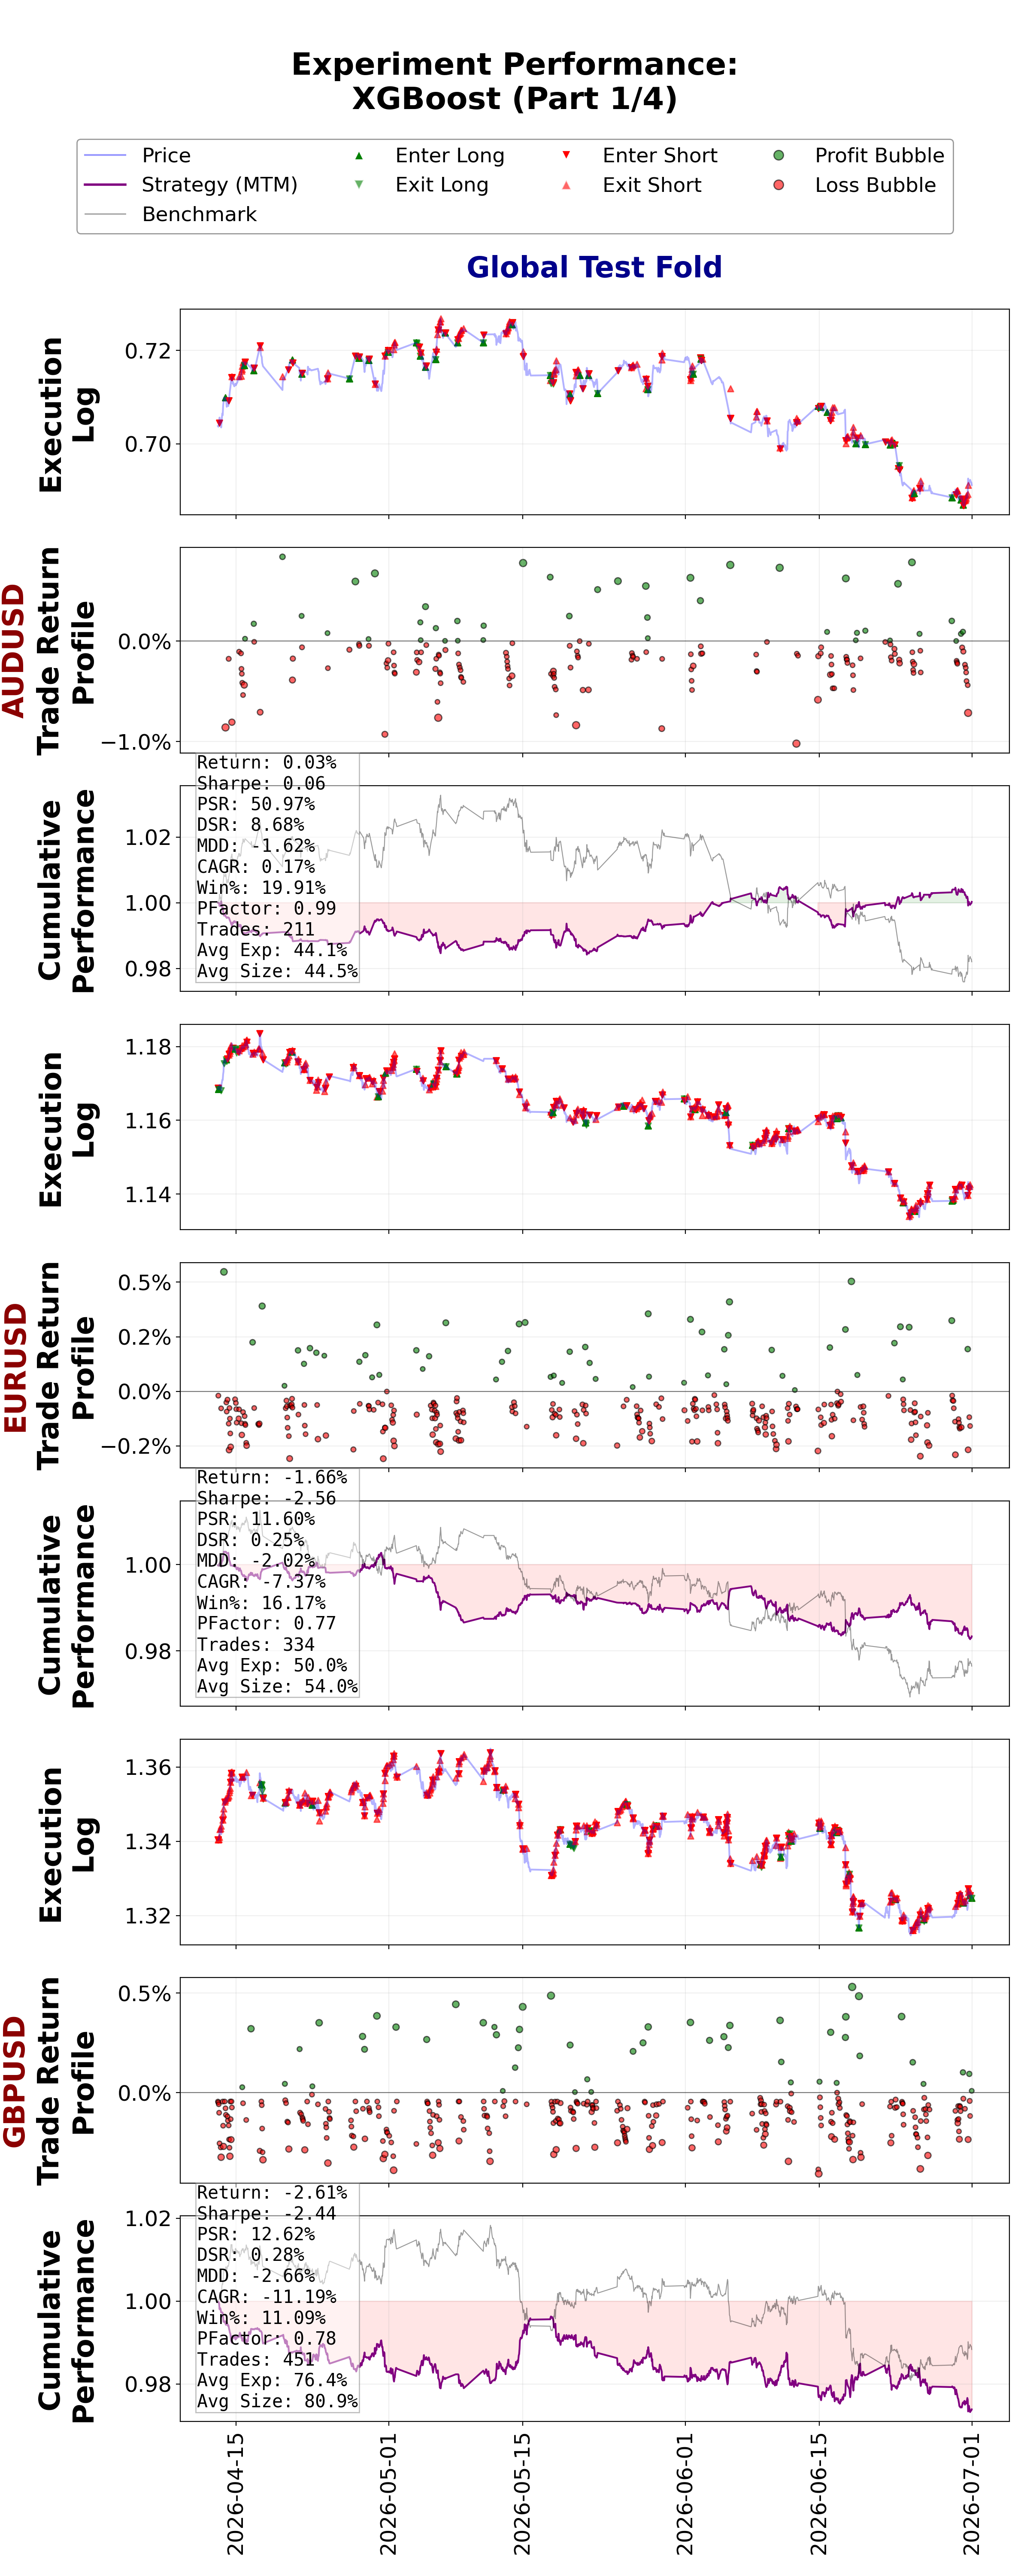
\includegraphics[width=\textwidth]{../data/figures/backtests/experiment_results_XGBoost_part1.png}
        \caption{Backtest Result of XGBoost During Production Experiment}
        \label{fig:production_experiment_result_XGBoost_1}
    \end{minipage}
    \hfill
    \begin{minipage}[t]{0.49\textwidth}
        \centering
        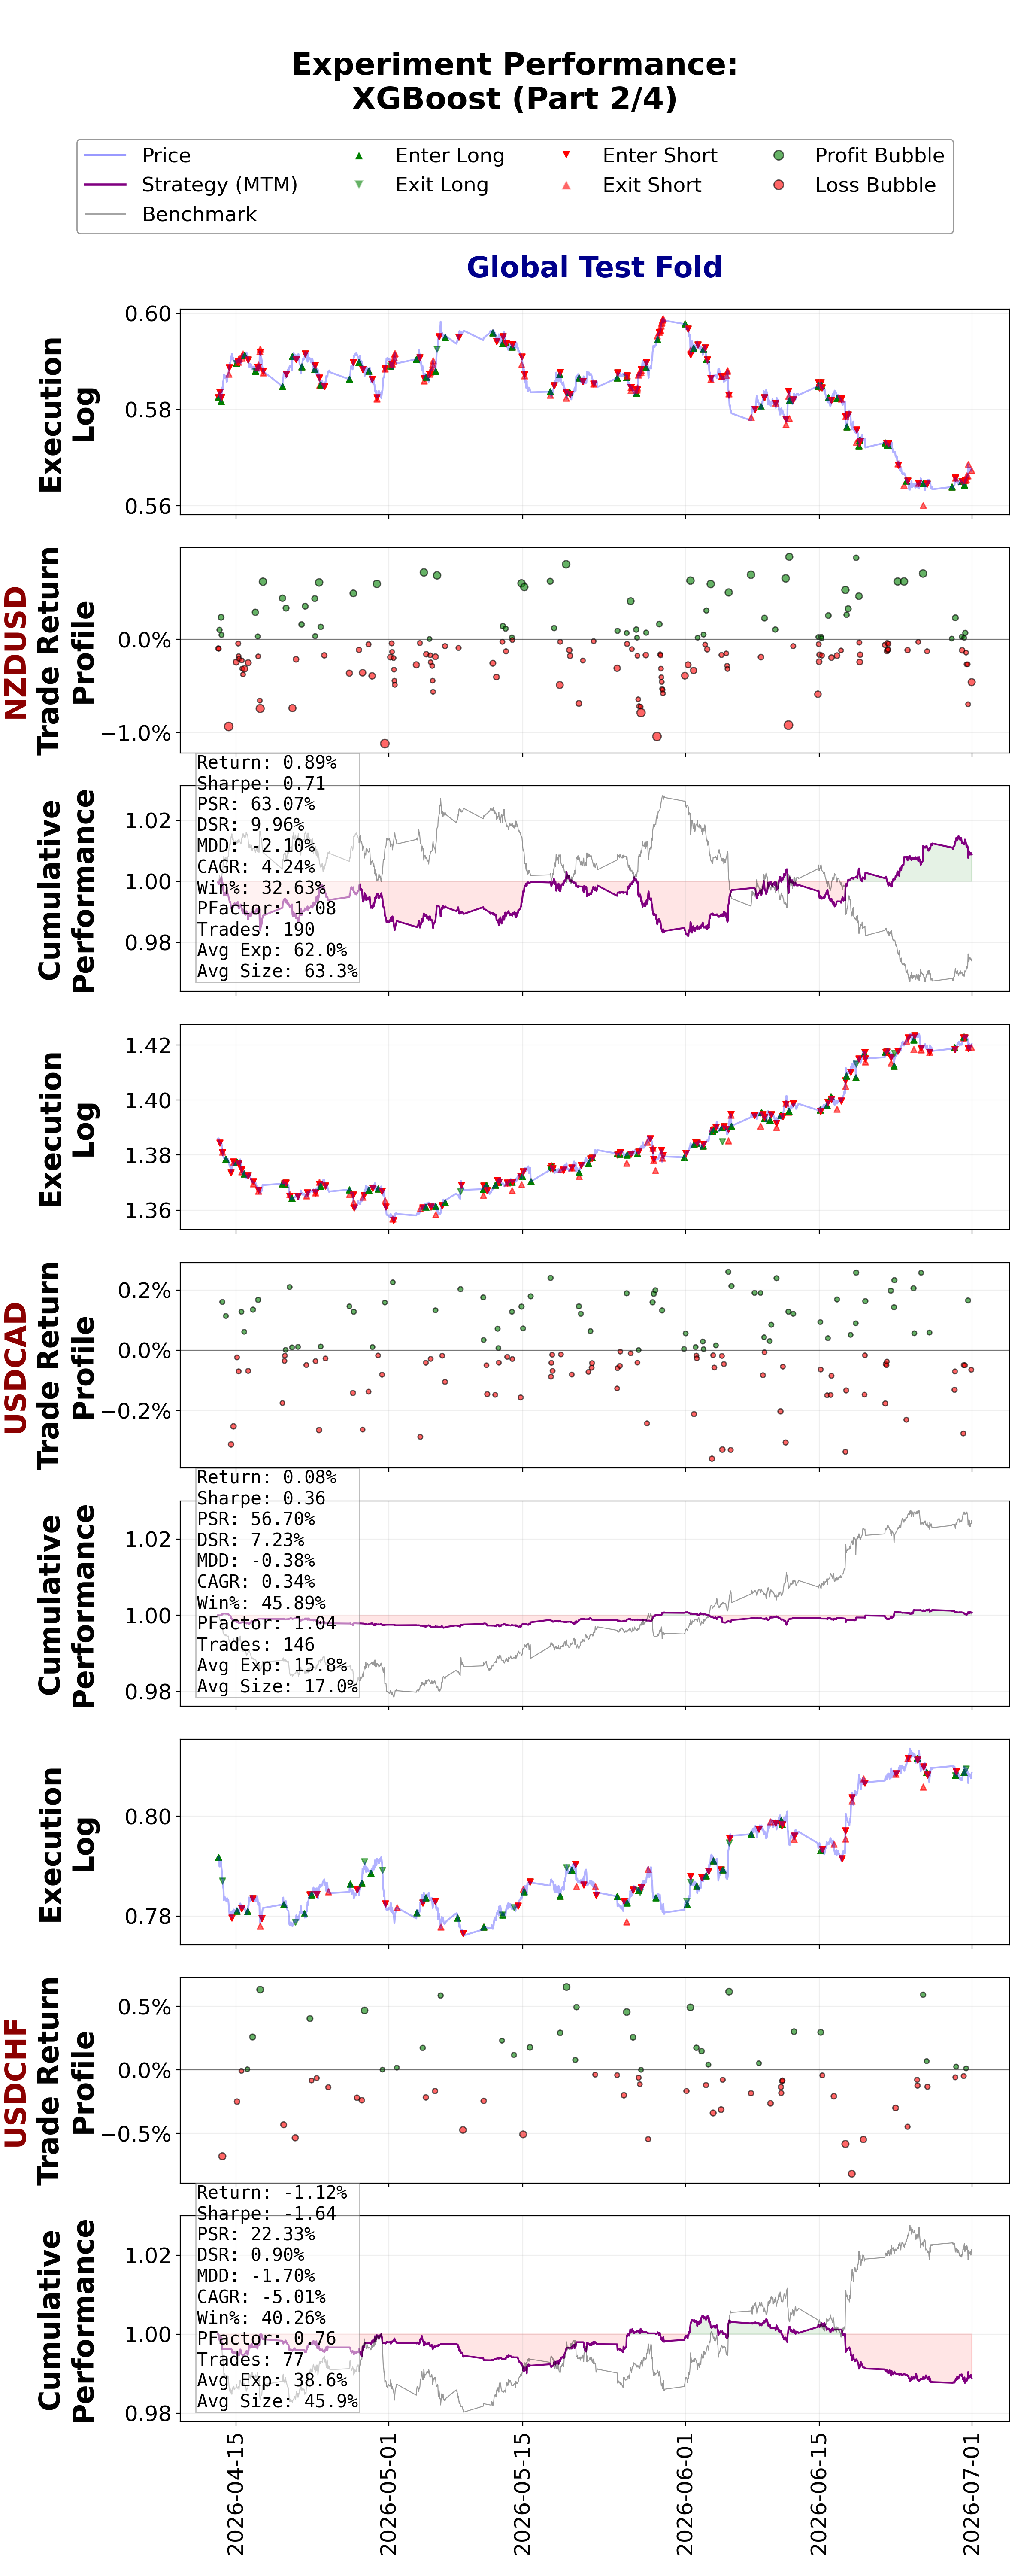
\includegraphics[width=\textwidth]{../data/figures/backtests/experiment_results_XGBoost_part2.png}
        \caption{Backtest Result of XGBoost During Production Experiment (Continued)}
        \label{fig:production_experiment_result_XGBoost_2}
    \end{minipage}
\end{figure}

\begin{figure}[H]
    \centering
    \begin{minipage}[t]{0.49\textwidth}
        \centering
        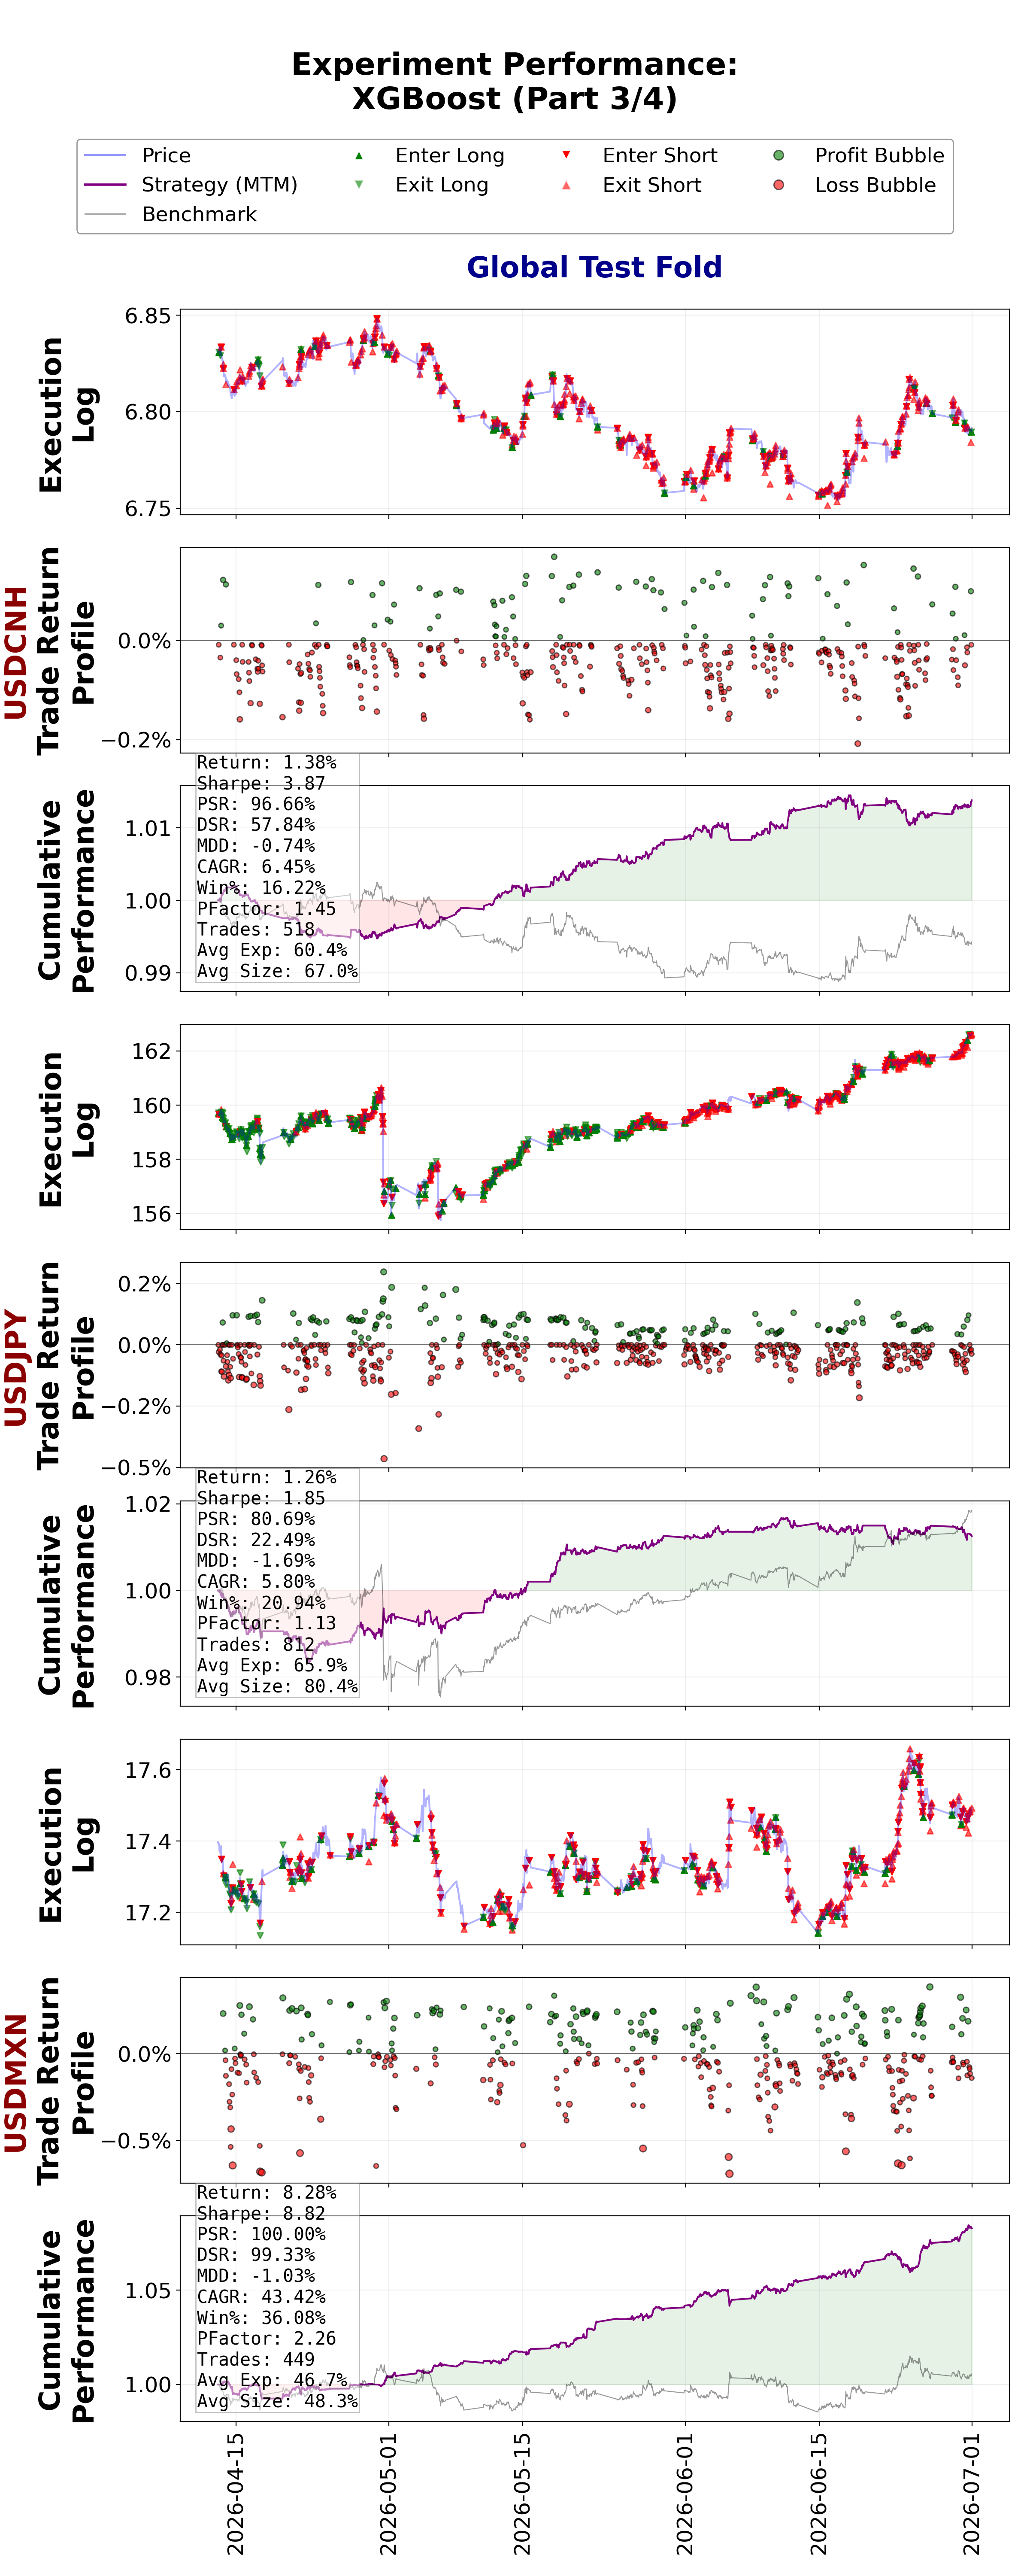
\includegraphics[width=\textwidth]{../data/figures/backtests/experiment_results_XGBoost_part3.png}
        \caption{Backtest Result of XGBoost During Production Experiment (Continued)}
        \label{fig:production_experiment_result_XGBoost_3}
    \end{minipage}
    \hfill
    \begin{minipage}[t]{0.49\textwidth}
        \centering
        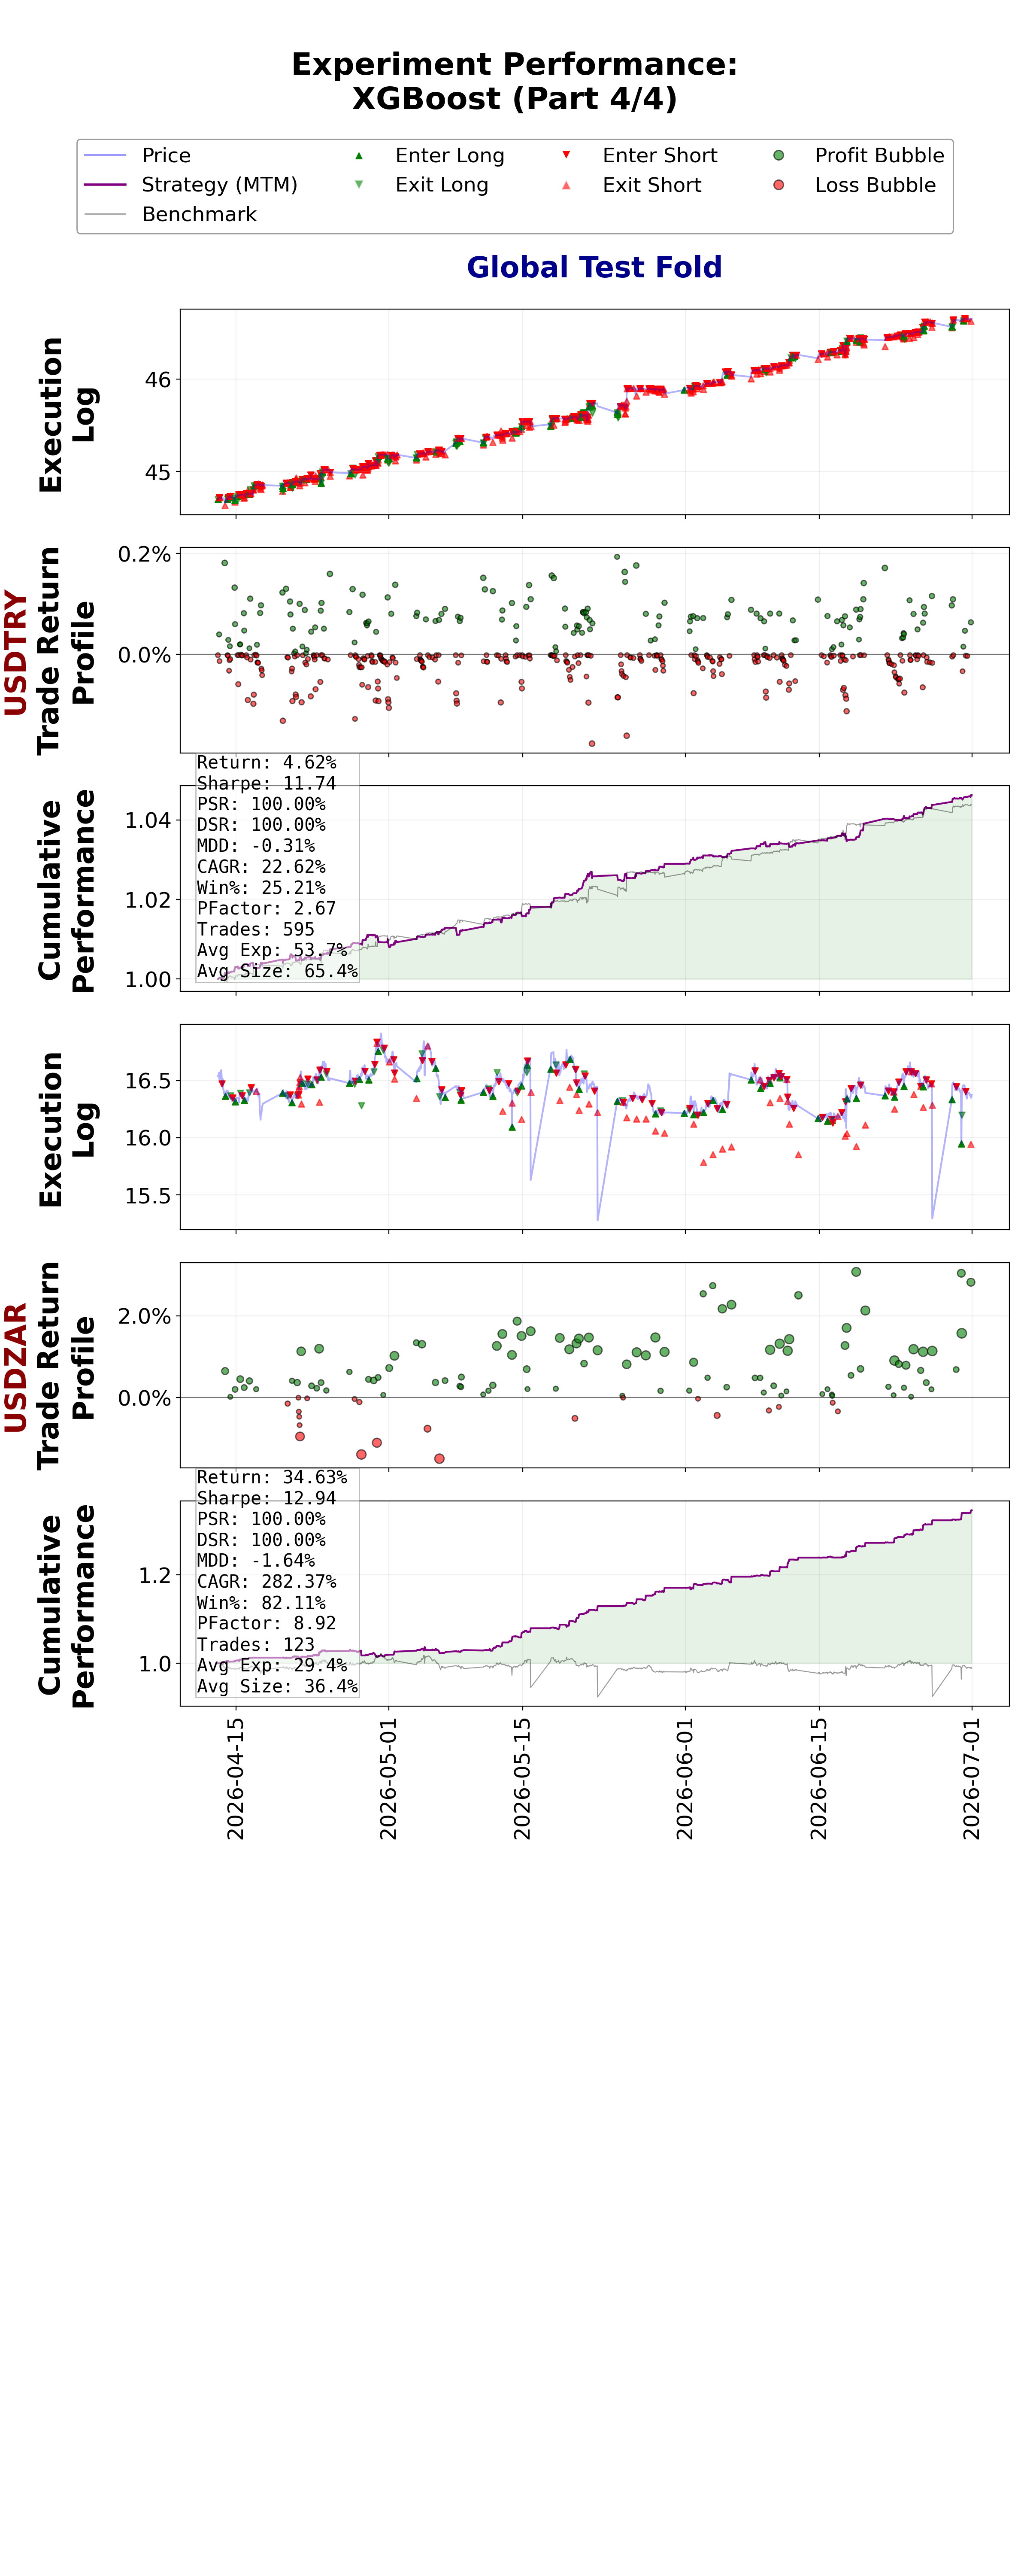
\includegraphics[width=\textwidth]{../data/figures/backtests/experiment_results_XGBoost_part4.png}
        \caption{Backtest Result of XGBoost During Production Experiment (Continued)}
        \label{fig:production_experiment_result_XGBoost_4}
    \end{minipage}
\end{figure}


%%%%%%%%%%%%%%%%%%%%%%%%%%%%%%%%%%%%%%%%%%%%%%%%%%%%%%%%%%%%%%%%%%%%%%%%%%%%%%%%%%%%%%%%%%%%%
%%%%%%%%%%%%%%%%%%%%%%%%%%%%%%%%%%%%%%%%%%%%%%%%%%%%%%%%%%%%%%%%%%%%%%%%%%%%%%%%%%%%%%%%%%%%%
%%%%%%%%%%%%%%%%%%%%%%%%%%%%%%%%%%%%%%%%%%%%%%%%%%%%%%%%%%%%%%%%%%%%%%%%%%%%%%%%%%%%%%%%%%%%%

\subsection{Synthesis: Revisiting the Overarching Research Question}

Bringing these five threads together, this thesis's answer to whether an ML classifier can drive a Forex trading model successfully is layered. A raw classifier cannot as the M1-only 
dissection is the single most unambiguous result in the entire empirical chapter (see table \ref{tab:strategy_comparison_XGBoost_tournament}). A classifier embedded in a meta-labeling 
and conformal veto architecture can be made profitable on a subset of its trading universe, but the mechanism by which it becomes profitable is disproportionately one of principled 
abstention to trade rather than improved directional accuracy. Also, the profits that remain are concentrated in a small number of EM/exotic pairs whose statistics are, on closer 
inspection, considerably more fragile (event-dependent, small-sample, DSR-flagged, or exhibit data integrity issues) than their headline Sharpe ratios suggest. The tournament 
framework succeeded at its narrower, comparative task of identifying the least fragile of six candidates under a shared adversarial protocol, but neither the tournament nor the 
production refit produced an architecture whose success generalizes uniformly across the full multi-pair universe. The per-pair local adaptation this thesis set out to test remains 
only partially and inconsistently supported by the dissection evidence gathered. Taken as a whole, we regard this as a more honest and more useful finding than a simple confirmation 
of the original hypothesis would have been, since it identifies precisely which components of the pipeline (the veto logic, the per-pair significance threshold) are doing genuine, 
traceable work, and which components (uniform cross-pair profitability, the incremental benefit of local trading-parameter tuning over a global configuration) remain unresolved and 
should not be oversold on the strength of this study's two-fold, short evaluation alone.

%%%%%%%%%%%%%%
% CONCLUSION %
%%%%%%%%%%%%%%
\section{Conclusion and Future Work}
\subsection{Summary}

This thesis set out to answer a deliberately blunt question, whether a machine learning classifier can be built that drives a Forex trading model successfully. Rather than pursuing 
raw predictive power, the approach taken here was to treat that question as one of statistical verification first and prediction second, building a pipeline in which every candidate 
trade signal has to survive a sequence of adversarial checks, a nested walk-forward split, a secondary meta-model acting as referee, a conformal calibration layer 
translating that referee's opinion into a formal significance test, and a deflated Sharpe ratio correcting for the number of configurations searched along the way, before it is 
allowed to reach the backtester at all.

\medskip

Across the five research objectives, the results are consistent in shape even where they differ in detail, because this machinery matters, and it matters in a specific way. The 
architecture tournament (Objective 1) identified XGBoost as the most defensible candidate among six architectures, not because it traded profitably everywhere, none of the six 
did, but because its conformal calibration held up more reliably than its competitors' and its failure modes remained traceable rather than hidden. The meta-labeling and conformal 
filtering layer (Objective 2) turned out to be the single load-bearing component of the entire pipeline as an unfiltered directional signal was not merely weak but actively 
loss-making and the recovery into profitability came almost entirely from the system learning when not to trade rather than from any improvement in directional accuracy. Statistical 
discovery control via the deflated Sharpe ratio (Objective 3) did its intended job of separating likely noise from likely signal, flagging two of the production model's nominally 
profitable pairs as statistically indistinguishable from chance, though it was equally clear that a high DSR is a defense against selection bias in hyperparameter search and not a 
guarantee of a stationary, repeatable edge. The feature post-mortem (Objective 4) surfaced a small, stable core of momentum and microstructure features that held their rank across 
both out-of-sample windows, alongside a much larger set of features whose importance reshuffled substantially fold to fold, which is a pattern that shaped the tournament's design as 
much as it did its results. Ultimately, the question of global robustness versus local adaptation (Objective 5) was answered unevenly under the current pipeline, since the 
pair-specific conformal significance threshold did real, decisive work by driving the model to almost entirely avoid G7 majors, while the corresponding case for pair-specific 
trading parameter tuning over a single global configuration remained genuinely unresolved across the two folds tested.

\medskip

Taken together, this thesis does not conclude that machine learning can drive a uniformly profitable Forex strategy across the subset of eleven pairs and the empirical record does 
not support that stronger claim. What it does show is narrower and, we think, more useful, because a classifier-driven pipeline can be made to behave responsibly under out-of-sample 
testing, largely by being taught to say no. The resulting, concentrated profitability that remains is real enough to survive a battery of overfitting checks in a handful of 
pairs, while being modest, fragile, and event-dependent enough that it should be read as a proof of concept for the verification framework itself rather than as evidence of a 
deployable, general-purpose trading edge. If there is a single takeaway this research would want to leave a practitioner or a future researcher with, it is that the statistical 
skepticism built into the pipeline, the willingness to reject a signal, a pair, or an entire architecture rather than force a result, is not a constraint on this approach's 
performance but the mechanism that makes whatever performance does emerge worth taking seriously in the first place.


\subsection{Future Extensions}

\subsubsection{Refactoring of the Codebase}

The current implementation, while functionally adequate for the scope of this thesis, is organized as a set of tightly connected, procedural scripts rather than a 
modular software architecture. Data acquisition, model training, conformal calibration, and order execution are frequently interleaved within the same function 
bodies and share mutable state across long-running loops, which makes unit testing individual components in isolation difficult. 
A more maintainable direction, sketched in \ref{app:code refactored}, would separate the system into a domain layer of data classes 
(MarketData and Signal), and three interfaces for data acquisition, strategy generation, and execution, which will be coordinated through a thin 
TradingSystemFacade. Under this design, concrete implementations (e.g. an IBKR\_MarketDataFeed or a BacktestSimEngine) become interchangeable behind their 
respective interfaces (IDataProvider and IExecutionEngine), allowing the same strategy logic to run unmodified against a live broker or a historical simulation. 
Furthermore, the conformal veto could similarly be expressed as a decorator (ConformalVetoDecorator) wrapping an inner IStrategy, rather than being hard-coded into 
the signal generation path. It should be stressed that this diagram is illustrative rather than a finished architecture and is intended merely to gesture toward the 
SOLID design principles, adherence to which was not a concern of this thesis. Adopting such a structure would not, by itself, resolve the statistical subtleties 
uncovered in this study but rather it would reduce the engineering risk of introducing or hiding such issues in the first place, while meaningfully easing the 
future extensions proposed below.


\subsubsection{Data Quality}

While this study maintains high standards for data integrity through rigorous sanity checks (\ref{sec:sanity_checks}), a primary area for future extension is the further hardening of the 
underlying data source. Our current pipeline orchestrates the merging of Polygon.io (via OpenBB) for primary transaction data and Dukascopy for binary-decoded bid/ask spreads
and thus relies on a naive UTC timestamp synchronization (see \ref{sec:data_acquisition}). While every precaution was taken to ensure temporal alignment, the lack of a unified,
high-precision institutional primary key (such as millisecond-accurate FIX sequence numbers) leaves a non-zero margin for micro-gaps or off-by-one errors during the left-join process.
Consequently, future research should explore the utilization of a unified institutional liquidity provider (e.g., LMAX Exchange, Bloomberg, or Interactive Brokers' IDB feed). 
Sourcing transaction prices and spreads from a single engine would eliminate the need for heuristic temporal merging and provide a more robust ground truth for the M2 meta-model. 
Furthermore, extending the dataset to include tick-level order flow (Level 2 data) would allow the meta-model to move beyond simple OHLCV features and audit the efficacy of the conformal 
veto logic within the context of market depth and order book imbalances.


\subsubsection{More Insightful Feature Engineering}

A primary limitation of the feature engineering framework discussed in \ref{sec:features_labels} is its exclusive reliance on endogenous variables. 
While our current suite of, among others, momentum, volatility, and microstructural indicators provides a high-fidelity mapping of the instrument's own price-action
dynamics, it operates within a macroeconomic vacuum. In the highly integrated global Forex market, currency valuations are fundamentally driven by inter-market relative value and 
sovereign yield differentials. To move beyond the limitations of univariate price analysis, future extensions should incorporate exogenous features that capture the broader economic landscape. 
Specifically, the integration of interest rate differentials (using 2-year and 10-year Treasury yield spreads), global equity market volatility (VIX), and commodity price indices 
(e.g., WTI Crude for the CAD, or Gold for the AUD) could provide the meta-model with critical market regime context. These data streams could be sourced through high-frequency 
macroeconomic APIs such as the Federal Reserve Economic Data (FRED) or Refinitiv Eikon. By augmenting the M1 signal generator with these external pressures, the meta-model (M2)
could develop a more nuanced understanding of when a technical signal is aligned with or fighting against fundamental capital flows, thereby further refining the efficacy of the 
conformal veto logic.

\subsubsection{More Exhaustive Hyperparameter Search}

% For tournament
% n_model_trials=25        # Number of 'outer' Optuna trials to conduct (computationally expensive because it involves Model training)
% n_trading_trials=50     # Number of 'inner' Optuna trials to conduct (conducts n backtests on the same model for fair evaluation)

% For productionn_model_trials=50        # Number of 'outer' Optuna trials to conduct (computationally expensive because it involves Model training)
% n_trading_trials=100     # Number of 'inner' Optuna trials to conduct (conducts n backtests on the same model for fair evaluation)

%%%%%%%%%%%%%%%%
% BIBLIOGRAPHY %
%%%%%%%%%%%%%%%%
\section{References}
\printbibliography[heading=none]

%%%%%%%%%%%%
% APPENDIX %
%%%%%%%%%%%%
\section{Appendix}
\appendix


\section{Evaluation Metrics}\label{app:metrics}

The primary measure of risk-adjusted return is the Sharpe Ratio, which we calculate using arithmetic returns \( r_t = \frac{(E_t - E_{t-1})}{E_{t-1}} \). 
To ensure comparability across different time horizons, the ratio is annualized as follows:

\begin{equation}
    \text{SR} = \frac{\overline{r}}{\sigma_{r}} \times \sqrt{N}
    \label{eq:sharpe_ratio}
\end{equation}

where $\overline{r}$ is the mean return, $\sigma_{r}$ is the standard deviation of returns, and N is the annualization factor (i.e., N=252 $\times$ 24 for hourly data).
Unlike simple average returns, the compund annual growth rate (CAGR) represents the annualized geometric mean return that would provide the same final equity from the initial capital over time, 
accounting for the compounding effect:

\begin{equation}
    \text{CAGR} = \left( \frac{E_T}{E_0} \right)^{\frac{1}{y}} - 1
    \label{eq:cagr}
\end{equation}

where $E_T$ is the final equity, $E_0$ is the initial capital, and y is the total elapsed time in years.
The maximum drawdown (MDD) measures the largest peak-to-trough decline in the account's history, serving as the primary indicator of absolute risk and investor pain:

\begin{equation}
    \text{MDD} = \max_{0 \leq t \leq T} \left( \frac{ \max_{0 \leq \tau \leq t} E_\tau - E_t }{ \max_{0 \leq \tau \leq t} E_\tau } \right)
    \label{eq:mdd}
\end{equation}

where \(E_t\) is the equity at time \(t\), \(T\) is the total evaluation period, and \(\tau\) indexes all time points from the start up to the current time \(t\). 
The inner maximum identifies the historical peak up to time \(t\), and the expression computes the percentage decline from that peak to the current equity \(E_t\). 
The outer maximum then selects the largest such decline over the entire period.
The profit factor (PF) measures the net profitability relative to net losses, providing a simple way to evaluate whether a strategy generates more profit than loss:

\begin{equation}
    \text{PF} = \frac{\sum_{i=1}^{n} \text{PnL}_i \cdot \mathbf{1}_{\{\text{PnL}_i > 0\}}}{\sum_{i=1}^{n} \left\|\text{PnL}_i\right\| \cdot \mathbf{1}_{\{\text{PnL}_i < 0\}}}
    \label{eq:profit_factor}
\end{equation}

where \(\text{PnL}_i\) is the net profit or loss of the \(i\)-th trade (or period), \(n\) is the total number of trades. The numerator sums only positive outcomes, 
while the denominator sums the absolute values of negative outcomes. A profit factor greater than 1 indicates a profitable strategy, whereas below 1 indicates a losing strategy.
The win rate (WR) represents the proportion of trades that result in a net profit after accounting for all transaction costs, including both entry and exit fees as well as slippage. 
Unlike a simple percentage of price-positive trades, this definition requires that the net round-trip profit strictly exceeds zero:

\begin{equation}
    \text{WR} = \frac{1}{n} \sum_{i=1}^{n} \mathbf{1}_{\{\text{PnL}_i > 0\}}
    \label{eq:win_rate}
\end{equation}

where \(n\) is the total number of completed round-trip trades, \(\text{PnL}_i\) is the net profit or loss of the \(i\)-th trade after deducting both entry and exit transaction costs and 
slippage, and \(\mathbf{1}_{\{\cdot\}}\) is the indicator function that equals 1 if the condition inside is true and 0 otherwise. 
A win is strictly defined as \(\text{PnL}_i > 0\) such that trades with exactly zero net profit are not counted as wins. The win rate ranges from 0 to 1, 
with higher values indicating a greater proportion of net-profitable trades.
The instantaneous exposure at time \(t\) is defined as the percentage of mark-to-market equity that is deployed in active positions:

\begin{equation}
    \text{Exp}_t = \frac{\text{Notional}_t}{\text{E}_t} \times 100
    \label{eq:exposure}
\end{equation}

where \(\text{Notional}_t\) is the total notional value of the open position at time \(t\) (calculated as $\|\text{Bet} \times \text{Entry Price}\|$), and 
\(\text{E}_t\) is the mark-to-market account equity at time \(t\). Exposure values range from 0\% (fully in cash) to potentially over 100\% if leverage is employed.
The average capital exposure (ACE) measures the time-weighted average percentage of account equity deployed in the market throughout the entire evaluation period, 
including periods when the strategy is entirely in cash:

\begin{equation}
    \text{ACE} = \frac{1}{T} \sum_{t=1}^{T} \text{Exp}_t
    \label{eq:avg_capital_exposure}
\end{equation}

where \(T\) is the total number of bars in the simulation and \(\text{Exp}_t\) is the instantaneous notional exposure at time \(t\) as a percentage of mark-to-market equity. 
This metric provides a holistic view of the strategy's "market presence". A low ACE indicates a highly selective strategy that spends significant time in cash, whereas a high ACE reflects 
a strategy with a frequent or persistent market footprint.
The average trade size (ATS) quantifies the average capital commitment only during active trading periods. Unlike ACE, this metric excludes all bars where the portfolio is neutral, 
thereby isolating the average intensity of the strategy's market participation when a position is actually held:

\begin{equation}
    \text{ATS} = \frac{\sum_{t=1}^{T} \text{Exp}_t \cdot \mathbf{1}_{\{\text{Exp}_t > 0\}}}{\sum_{t=1}^{T} \mathbf{1}_{\{\text{Exp}_t > 0\}}}
    \label{eq:avg_trade_size}
\end{equation}

where \(\text{Exp}_t\) is the instantaneous exposure and \(\mathbf{1}_{\{\cdot\}}\) is the indicator function. The denominator represents the total number of bars during which the 
strategy held an active position (\(\text{Exp}_t > 0\)). This metric is critical for evaluating the "typical" risk profile of the strategy's active bets, 
specifically how risk-management guardrails and conformal conviction scaling modulate position sizes in accordance with the strength of the statistical evidence.
The minimum track record length (MinTRL) defines the number of observations required to reject the null hypothesis that the observed Sharpe ratio is less than or equal to a target 
benchmark \(\text{SR}^*\) at a given significance level \(\alpha\). Developed by \textcite[see Eq. 13]{bailey_sharpe_2012}, MinTRL accounts for the non-normality of financial returns by 
incorporating the skewness and kurtosis of the return distribution:

\begin{equation}
    \text{MinTRL} = 1 + \left[ 1 - \hat{\gamma}_3 \widehat{\text{SR}} + \frac{\hat{\gamma}_4 - 1}{4} \widehat{\text{SR}}^2 \right] \left( \frac{Z_{\alpha}}{\widehat{\text{SR}} - \text{SR}^*} \right)^2
    \label{eq:mintrl}
\end{equation}

where \(\widehat{\text{SR}}\) is the observed non-annualized Sharpe ratio, \(\text{SR}^*\) is the non-annualized benchmark Sharpe ratio (typically 0), 
\(\hat{\gamma}_3\) and \(\hat{\gamma}_4\) are the skewness and Pearson kurtosis of the returns respectively, and \(Z_{\alpha}\) is the critical value for the \(1-\alpha\) quantile of the 
standard normal distribution. This metric provides a critical verification hurdle for backtest results. If the actual duration of the simulation is shorter than the computed MinTRL, 
the observed performance is considered statistically insufficient to distinguish the strategy's edge from random chance.


\section{Tournament}\label{app:tournament}
\subsection{Tournament Feature Selection}\label{app:tourney_feat_select}

\begin{figure}[H]
    \centering
    \includegraphics[width=0.9\linewidth]{../data/figures/feature_selection/Tournament_nested_correlation_heatmap.png}
    \caption{Correlation Filtering During Tournament}
    \label{fig:correlation filtering}
\end{figure}


\subsection{Pair- and Model-Specific Parameter Discovery}
\input{../data/tables/tournament/trading_hps_table/hps_ExtraTrees_tournament.tex}
\input{../data/tables/tournament/trading_hps_table/hps_GRU_tournament.tex}
\input{../data/tables/tournament/trading_hps_table/hps_LightGBM_tournament.tex}
\input{../data/tables/tournament/trading_hps_table/hps_LSTM_tournament.tex}
\input{../data/tables/tournament/trading_hps_table/hps_RandomForest_tournament.tex}

\subsection{Model-Specific Backtest Results}\label{app:model_specific_backtests}
\begin{figure}[H]
    \centering
    \begin{minipage}[t]{0.49\textwidth}
        \centering
        \includegraphics[width=\textwidth]{../data/figures/backtests/tournament_results_ExtraTrees_part1.png}
        \caption{Backtest Result of ExtraTrees During Tournament}
        \label{fig:tournament_results_ExtraTrees_1}
    \end{minipage}
    \hfill
    \begin{minipage}[t]{0.49\textwidth}
        \centering
        \includegraphics[width=\textwidth]{../data/figures/backtests/tournament_results_ExtraTrees_part2.png}
        \caption{Backtest Result of ExtraTrees During Tournament (Continued)}
        \label{fig:tournament_results_ExtraTrees_2}
    \end{minipage}
\end{figure}

\begin{figure}[H]
    \centering
    \begin{minipage}[t]{0.49\textwidth}
        \centering
        \includegraphics[width=\textwidth]{../data/figures/backtests/tournament_results_ExtraTrees_part3.png}
        \caption{Backtest Result of ExtraTrees During Tournament (Continued)}
        \label{fig:tournament_results_ExtraTrees_3}
    \end{minipage}
    \hfill
    \begin{minipage}[t]{0.49\textwidth}
        \centering
        \includegraphics[width=\textwidth]{../data/figures/backtests/tournament_results_ExtraTrees_part4.png}
        \caption{Backtest Result of ExtraTrees During Tournament (Continued)}
        \label{fig:tournament_results_ExtraTrees_4}
    \end{minipage}
\end{figure}


\begin{figure}[H]
    \centering
    \begin{minipage}[t]{0.49\textwidth}
        \centering
        \includegraphics[width=\textwidth]{../data/figures/backtests/tournament_results_GRU_part1.png}
        \caption{Backtest Result of GRU During Tournament}
        \label{fig:tournament_results_GRU_1}
    \end{minipage}
    \hfill
    \begin{minipage}[t]{0.49\textwidth}
        \centering
        \includegraphics[width=\textwidth]{../data/figures/backtests/tournament_results_GRU_part2.png}
        \caption{Backtest Result of GRU During Tournament (Continued)}
        \label{fig:tournament_results_GRU_2}
    \end{minipage}
\end{figure}

\begin{figure}[H]
    \centering
    \begin{minipage}[t]{0.49\textwidth}
        \centering
        \includegraphics[width=\textwidth]{../data/figures/backtests/tournament_results_GRU_part3.png}
        \caption{Backtest Result of GRU During Tournament (Continued)}
        \label{fig:tournament_results_GRU_3}
    \end{minipage}
    \hfill
    \begin{minipage}[t]{0.49\textwidth}
        \centering
        \includegraphics[width=\textwidth]{../data/figures/backtests/tournament_results_GRU_part4.png}
        \caption{Backtest Result of GRU During Tournament (Continued)}
        \label{fig:tournament_results_GRU_4}
    \end{minipage}
\end{figure}


\begin{figure}[H]
    \centering
    \begin{minipage}[t]{0.49\textwidth}
        \centering
        \includegraphics[width=\textwidth]{../data/figures/backtests/tournament_results_LightGBM_part1.png}
        \caption{Backtest Result of LightGBM During Tournament}
        \label{fig:tournament_results_LightGBM_1}
    \end{minipage}
    \hfill
    \begin{minipage}[t]{0.49\textwidth}
        \centering
        \includegraphics[width=\textwidth]{../data/figures/backtests/tournament_results_LightGBM_part2.png}
        \caption{Backtest Result of LightGBM During Tournament (Continued)}
        \label{fig:tournament_results_LightGBM_2}
    \end{minipage}
\end{figure}

\begin{figure}[H]
    \centering
    \begin{minipage}[t]{0.49\textwidth}
        \centering
        \includegraphics[width=\textwidth]{../data/figures/backtests/tournament_results_LightGBM_part3.png}
        \caption{Backtest Result of LightGBM During Tournament (Continued)}
        \label{fig:tournament_results_LightGBM_3}
    \end{minipage}
    \hfill
    \begin{minipage}[t]{0.49\textwidth}
        \centering
        \includegraphics[width=\textwidth]{../data/figures/backtests/tournament_results_LightGBM_part4.png}
        \caption{Backtest Result of LightGBM During Tournament (Continued)}
        \label{fig:tournament_results_LightGBM_4}
    \end{minipage}
\end{figure}


\begin{figure}[H]
    \centering
    \begin{minipage}[t]{0.49\textwidth}
        \centering
        \includegraphics[width=\textwidth]{../data/figures/backtests/tournament_results_LSTM_part1.png}
        \caption{Backtest Result of LSTM During Tournament}
        \label{fig:tournament_results_LSTM_1}
    \end{minipage}
    \hfill
    \begin{minipage}[t]{0.49\textwidth}
        \centering
        \includegraphics[width=\textwidth]{../data/figures/backtests/tournament_results_LSTM_part2.png}
        \caption{Backtest Result of LSTM During Tournament (Continued)}
        \label{fig:tournament_results_LSTM_2}
    \end{minipage}
\end{figure}

\begin{figure}[H]
    \centering
    \begin{minipage}[t]{0.49\textwidth}
        \centering
        \includegraphics[width=\textwidth]{../data/figures/backtests/tournament_results_LSTM_part3.png}
        \caption{Backtest Result of LSTM During Tournament (Continued)}
        \label{fig:tournament_results_LSTM_3}
    \end{minipage}
    \hfill
    \begin{minipage}[t]{0.49\textwidth}
        \centering
        \includegraphics[width=\textwidth]{../data/figures/backtests/tournament_results_LSTM_part4.png}
        \caption{Backtest Result of LSTM During Tournament (Continued)}
        \label{fig:tournament_results_LSTM_4}
    \end{minipage}
\end{figure}


\begin{figure}[H]
    \centering
    \begin{minipage}[t]{0.49\textwidth}
        \centering
        \includegraphics[width=\textwidth]{../data/figures/backtests/tournament_results_RandomForest_part1.png}
        \caption{Backtest Result of RandomForest During Tournament}
        \label{fig:tournament_result_RandomForest_1}
    \end{minipage}
    \hfill
    \begin{minipage}[t]{0.49\textwidth}
        \centering
        \includegraphics[width=\textwidth]{../data/figures/backtests/tournament_results_RandomForest_part2.png}
        \caption{Backtest Result of RandomForest During Tournament (Continued)}
        \label{fig:tournament_result_RandomForest_2}
    \end{minipage}
\end{figure}

\begin{figure}[H]
    \centering
    \begin{minipage}[t]{0.49\textwidth}
        \centering
        \includegraphics[width=\textwidth]{../data/figures/backtests/tournament_results_RandomForest_part3.png}
        \caption{Backtest Result of RandomForest During Tournament (Continued)}
        \label{fig:tournament_result_RandomForest_3}
    \end{minipage}
    \hfill
    \begin{minipage}[t]{0.49\textwidth}
        \centering
        \includegraphics[width=\textwidth]{../data/figures/backtests/tournament_results_RandomForest_part4.png}
        \caption{Backtest Result of RandomForest During Tournament (Continued)}
        \label{fig:tournament_result_RandomForest_4}
    \end{minipage}
\end{figure}


\subsection{Granular Performance of Other Models}
\input{../data/tables/tournament/rrf_leaderboard/rrf_matrix_tournament.tex}
\input{../data/tables/tournament/performance_tables/perf_ExtraTrees_tournament.tex}
\input{../data/tables/tournament/performance_tables/perf_GRU_tournament.tex}
\input{../data/tables/tournament/performance_tables/perf_LightGBM_tournament.tex}
\input{../data/tables/tournament/performance_tables/perf_LSTM_tournament.tex}
\input{../data/tables/tournament/performance_tables/perf_RandomForest_tournament.tex}
\input{../data/tables/tournament/performance_tables/perf_XGBoost_tournament.tex}

\subsection{Strategy Comparison of Other Models}
\input{../data/tables/tournament/strategy_comparison/strategy_comp_ExtraTrees_tournament.tex}
\input{../data/tables/tournament/strategy_comparison/strategy_comp_GRU_tournament.tex}
\input{../data/tables/tournament/strategy_comparison/strategy_comp_LightGBM_tournament.tex}
\input{../data/tables/tournament/strategy_comparison/strategy_comp_LSTM_tournament.tex}
\input{../data/tables/tournament/strategy_comparison/strategy_comp_RandomForest_tournament.tex}


\section{Production Model}\label{app:prod model}
\subsection{Production Model Feature Selection}

\begin{figure}[H]
    \centering
    \includegraphics[width=0.95\linewidth]{../data/figures/feature_selection/Production_nested_correlation_heatmap.png}
    \caption{Correlation Filtering During Production}
    \label{fig:prod corr filter}
\end{figure}

\begin{figure}[H]
    \centering
    \includegraphics[width=0.95\linewidth]{../data/figures/feature_selection/Production_nested_feature_importances_RandomForest.png}
    \caption{Feature Importances During Production}
    \label{fig:prod featimp filter}
\end{figure}


\subsection{Production Model-Trading Parameter Cascade}

\begin{figure}[H]
    \centering
    \includegraphics[width=0.95\linewidth]{../data/figures/optimization/distributions/Production_financial_dist_XGBoost.png}
    \caption{Financial Statistic Distributions During Production Optimization}
    \label{fig:prod stat distributions}
\end{figure}

\begin{figure}[H]
    \centering
    
\includegraphics[width=0.95\linewidth]{../data/figures/optimization/production/XGBoost/param_importance_trading_(best)_xgboost.png}
    \caption{Optimization Parameter Importance Trading (Best) XGBoost}
    \label{fig:opt param importance trading rf}
\end{figure}


\subsection{Conformal Filtering}

\begin{figure}[H]
    \centering
    \includegraphics[width=0.7\linewidth]{../data/figures/conformal_predictions/Production_conformal_predictions.png}
    \caption{Model-Specific Conformal Filtering During Production}
    \label{fig:prod conf preds}
\end{figure}


\subsection{Confusion Matrices}

\begin{figure}[H]
    \centering
    \includegraphics[width=0.95\linewidth]{../data/figures/confusion_matrices/Production_nested_confusion_matrices.png}
    \caption{Model-Specific Confusion Matrices During Production}
    \label{fig:prod confusion matrices}
\end{figure}


\subsection{Reliability Diagrams}

\begin{figure}[H]
    \centering
    \includegraphics[width=0.5\linewidth]{../data/figures/reliability_diagrams/Production_reliability_diagrams.png}
    \caption{Model-Specific Reliability Diagrams During Production}
    \label{fig:prod reliability curves}
\end{figure}


\subsection{Granular Performance of Production Model}
\input{../data/tables/production/rrf_leaderboard/rrf_matrix_production.tex}
\input{../data/tables/production/rrf_leaderboard/rrf_summary_production.tex}
\input{../data/tables/production/performance_tables/perf_XGBoost_production.tex}


\section{Miscellaneous}\label{app:miscellaneous}
\subsection{Refactored Codebase}\label{app:code refactored}

\begin{sidewaysfigure}[htbp]
    \centering
    \includegraphics[width=\textheight]{../data/figures/refactored_code/code_refactored.png}
    \caption{Proposed Refactoring of the Codebase}
    \label{fig:refactor}
\end{sidewaysfigure}

\end{document}